\documentclass{amsart}
\usepackage{amsmath}
\usepackage{amssymb}
\usepackage{amsthm}
\newtheorem{thm}{定理}[section]
\newtheorem{cor}[thm]{推论}
\newtheorem{prop}[thm]{命题}
\newtheorem{lem}[thm]{引理}
\newtheorem{conj}[thm]{猜想}
\newtheorem{quest}[thm]{问题}
\newtheorem{claim}[thm]{断言}

\theoremstyle{definition}
\newtheorem{defn}[thm]{定义}
\newtheorem{defns}[thm]{定义}
\newtheorem{con}[thm]{构造}
\newtheorem{exm}[thm]{例}
\newtheorem{exms}[thm]{例}
\newtheorem{notn}[thm]{记号}
\newtheorem{notns}[thm]{记号}
\newtheorem{addm}[thm]{补充}
\newtheorem{exer}[thm]{习题}

\theoremstyle{remark}
\newtheorem{rmk}[thm]{注}
\newtheorem{rmks}[thm]{注}
\newtheorem{warn}[thm]{警告}
\newtheorem{sch}[thm]{评注}


% unnumbered theorems
\theoremstyle{plain}
\newtheorem*{thm*}{定理}
\newtheorem*{prop*}{命题}
\newtheorem*{lem*}{引理}
\newtheorem*{cor*}{推论}
\newtheorem*{conj*}{猜想}

% unnumbered definitions
\theoremstyle{definition}
\newtheorem*{defn*}{定义}
\newtheorem*{exer*}{习题}
\newtheorem*{defns*}{定义}
\newtheorem*{con*}{构造}
\newtheorem*{exm*}{例}
\newtheorem*{exms*}{例}
\newtheorem*{notn*}{记号}
\newtheorem*{notns*}{记号}
\newtheorem*{addm*}{补充}


\theoremstyle{remark}
\newtheorem*{rmk*}{注}
%\usepackage{MnSymbol}
\usepackage{bm}
\usepackage{accents}
\usepackage{mathtools}
\usepackage{tikz}
\usetikzlibrary{calc}
\usetikzlibrary{decorations.pathmorphing,shapes}
\usetikzlibrary{automata,positioning}
\usepackage{tikz-cd}
\usepackage{forest}
\usepackage{braket} 
\usepackage{listings}
\usepackage{mdframed}
\usepackage{verbatim}
\usepackage{physics2}
\usephysicsmodule{ab,ab.legacy,diagmat,xmat}
\usepackage{derivative}
\usepackage{fixdif}
\usepackage{stmaryrd}
% \usepackage{euscript} 
% \usepackage[mathcal]{eucal}
\usepackage{stackengine} 
%\usepackage{/home/patrickl/homework/macaulay2}

%font
\usepackage[sc]{mathpazo}
\usepackage{inconsolata}
\usepackage{microtype}
% \usepackage{fontspec} 
% \setmainfont{Tex Gyre Pagella}
\usepackage[OT1,euler-digits]{eulervm}
% \usepackage{euler-math} 
\usepackage[scaled=0.86]{berasans}
% \let\sffamilyold\sffamily
% \def\sffamily{\fontencoding{T1}\sffamilyold}
% \setmonofont{Inconsolatazi4}

% Chinese support
\usepackage{xeCJK}
\setCJKmainfont{Songti SC}
\setCJKsansfont{Heiti SC}
\setCJKmonofont{Songti SC}
\XeTeXlinebreaklocale "zh"
\XeTeXlinebreakskip = 0pt plus 1pt

%CS packages
\usepackage{algorithmicx}
\usepackage{algpseudocode}
\usepackage{algorithm}

% typeset and bib
\usepackage[english]{babel} 
% \usepackage[utf8]{inputenc} 
% \usepackage[T1]{fontenc}
\usepackage[backend=biber,style=alphabetic,maxalphanames=4,maxnames=5,hyperref,isbn=false]{biblatex}
\usepackage[bookmarks, colorlinks, breaklinks]{hyperref} 
\hypersetup{linkcolor=blue,citecolor=magenta,filecolor=black,urlcolor=blue}
\usepackage{cleveref}
\usepackage{graphicx}
\graphicspath{{./}}


% other formatting packages
\usepackage{float}
\usepackage{booktabs}
\usepackage[shortlabels]{enumitem}
\setitemize{noitemsep}
\usepackage{csquotes}
%\usepackage{titlesec}
%\usepackage{titling}
%\usepackage{fancyhdr}
%\usepackage{lastpage}
% \usepackage{parskip}
\newlist{mydescription}{description}{1}
\setlist[mydescription]{style=nextline,
                        font=\bfseries,
                        % Tweak the next 4 options as needed:
                        labelindent=1cm, 
                        leftmargin =2cm,
                        rightmargin=1cm,
                        topsep     =1ex
                       }
\setcounter{tocdepth}{1}
\usepackage{lipsum}

% delimiters
\DeclarePairedDelimiter{\gen}{\langle}{\rangle}
\DeclarePairedDelimiter{\floor}{\lfloor}{\rfloor}
\DeclarePairedDelimiter{\ceil}{\lceil}{\rceil}



% The theorem-like environments above all share the `thm' counter, so cleveref
% names every one of them ``Theorem'' and cannot format lists of them. Alias the
% counter back to each environment and give cleveref the names.
\usepackage{etoolbox}
\crefname{thm}{定理}{定理}
\Crefname{thm}{定理}{定理}
\crefname{defn}{定义}{定义}
\Crefname{defn}{定义}{定义}
\crefname{exm}{例}{例}
\Crefname{exm}{例}{例}
\crefname{rmk}{注}{注}
\Crefname{rmk}{注}{注}
\crefname{equation}{式}{式}
\Crefname{equation}{式}{式}
\crefname{figure}{图}{图}
\Crefname{figure}{图}{图}
\crefname{table}{表}{表}
\Crefname{table}{表}{表}
\crefformat{section}{第~#1~节}
\Crefformat{section}{第~#1~节}
\crefformat{subsection}{第~#1~小节}
\Crefformat{subsection}{第~#1~小节}
\AtBeginEnvironment{conj}{\crefalias{thm}{conj}}
\AtBeginEnvironment{prop}{\crefalias{thm}{prop}}
\AtBeginEnvironment{lem}{\crefalias{thm}{lem}}
\AtBeginEnvironment{cor}{\crefalias{thm}{cor}}
\crefname{conj}{猜想}{猜想}
\Crefname{conj}{猜想}{猜想}
\crefname{prop}{命题}{命题}
\Crefname{prop}{命题}{命题}
\crefname{lem}{引理}{引理}
\Crefname{lem}{引理}{引理}
\crefname{cor}{推论}{推论}
\Crefname{cor}{推论}{推论}

% shortcuts
\DeclareMathOperator{\Ima}{Im}
\newcommand{\A}{\mathbb{A}}
\newcommand{\G}{\mathbb{G}}
\newcommand{\N}{\mathbb{N}}
\newcommand{\R}{\mathbb{R}}
\newcommand{\C}{\mathbb{C}}
\newcommand{\Z}{\mathbb{Z}}
\newcommand{\Q}{\mathbb{Q}}
\newcommand{\E}{\mathbb{E}}
\newcommand{\V}{\mathbb{V}}
\renewcommand{\H}{\mathbb{H}}
\renewcommand{\k}{\Bbbk}
\renewcommand{\L}{\mathbb{L}}
\renewcommand{\P}{\mathbb{P}}
\newcommand{\M}{\mathcal{M}}
\newcommand{\Mbar}{\overline{\mathcal{M}}}
\newcommand{\g}{\mathfrak{g}}
\newcommand{\h}{\mathfrak{h}}
\newcommand{\n}{\mathfrak{n}}
\renewcommand{\b}{\mathfrak{b}}
\newcommand{\ep}{\varepsilon}
\newcommand*{\dt}[1]{%
   \accentset{\mbox{\Huge\bfseries .}}{#1}}
%\renewcommand{\abstractname}{Official Description}
\newcommand{\mc}[1]{\mathcal{#1}}
% \newcommand{\msc}[1]{\mathscr{#1}}
\newcommand{\T}{\mathbb{T}}
\newcommand{\mf}[1]{\mathfrak{#1}}
\newcommand{\mbf}[1]{\mathbf{#1}}
\newcommand{\bv}{\mbf{v}}
\newcommand{\bq}{\mbf{q}}
\newcommand{\bp}{\mbf{p}}
\newcommand{\btau}{\bm{\tau}}
\newcommand{\mr}[1]{\mathrm{#1}}
\newcommand{\on}[1]{\operatorname{#1}}
\newcommand{\ms}[1]{\mathsf{#1}}
\newcommand{\mt}[1]{\mathtt{#1}}
\newcommand{\ol}[1]{\overline{#1}}
\newcommand{\ul}[1]{\underline{#1}}
\newcommand{\wt}[1]{\widetilde{#1}}
\newcommand{\wh}[1]{\widehat{#1}}
\renewcommand{\div}{\operatorname{div}}
\newcommand{\1}{\mathbf{1}}
\newcommand{\2}{\mathbf{2}}
\newcommand{\3}{\mathbf{3}}
\newcommand{\I}{\mathrm{I}}
\newcommand{\II}{\mr{I}\hspace{-1.3pt}\mr{I}}
\newcommand{\III}{\mr{I}\hspace{-1.3pt}\mr{I}\hspace{-1.3pt}\mr{I}}
\renewcommand{\v}{\mbf{v}}
\newcommand{\w}{\mbf{w}}
\newcommand{\bmu}{\bm{\mu}}
\newcommand{\pre}{\mr{pre}}
\newcommand{\vir}{\mr{vir}}
\newcommand{\fl}{\mr{fl}}
\newcommand{\ps}[1]{\llbracket #1 \rrbracket}
\newcommand{\ls}[1]{\llparenthesis #1 \rrparenthesis}
\newcommand{\loc}{\mr{loc}}

\DeclareMathOperator{\Der}{Der}
\DeclareMathOperator{\Tor}{Tor}
\DeclareMathOperator{\Hom}{Hom}
\DeclareMathOperator{\End}{End}
\DeclareMathOperator{\Ext}{Ext}
\DeclareMathOperator{\ad}{ad}
\DeclareMathOperator{\Aut}{Aut}
\DeclareMathOperator{\Rad}{Rad}
\DeclareMathOperator{\Pic}{Pic}
\DeclareMathOperator{\NS}{NS}
\DeclareMathOperator{\supp}{supp}
\DeclareMathOperator{\Supp}{Supp}
\DeclareMathOperator{\depth}{depth}
\DeclareMathOperator{\sgn}{sgn}
\DeclareMathOperator{\spec}{Spec}
\DeclareMathOperator{\Spec}{Spec}
\DeclareMathOperator{\proj}{Proj}
\DeclareMathOperator{\Proj}{Proj}
\DeclareMathOperator{\ord}{ord}
\DeclareMathOperator{\Div}{Div}
\DeclareMathOperator{\Bl}{Bl}
\DeclareMathOperator{\coker}{coker}
\DeclareMathOperator{\ev}{ev}
\DeclareMathOperator{\st}{st}
\DeclareMathOperator{\pr}{pr}
\DeclareMathOperator{\ch}{ch}
\DeclareMathOperator{\Cont}{Cont}

\addbibresource{references.bib}

\title{对数 GLSM 及相关专题}
\author{Patrick Lei}
\date{\today}
\allowdisplaybreaks

\begin{document}
\renewcommand{\abstractname}{摘要}
\renewcommand{\contentsname}{目录}
\renewcommand{\refname}{参考文献}
    
\begin{abstract}
    这些笔记来自 2026 年 7 月在四川大学举办的对数 GLSM 暑期学校，为现场 TeX 速记稿（除我本人以及郭帅的报告之外，部分插图是事后使用 Codex 或 Claude Code 补入的）。请注意，所有报告（除我本人的以外）均以中文给出。若有任何翻译错误，以及我讲座中的任何错误，在此一并致歉。此外，郭帅两次讲座的笔记是依据其幻灯片生成的\textbf{实验性} AI 转录稿。虽然我已让 Claude 阅读了我的全部其他笔记以了解我的写作风格，但若发现文风不一致或任何错误，敬请告知。最后，感谢周祐正、方婷婷与温耀雄指出笔记中的错误。

    \medskip
    \noindent\textbf{译注：}本中文译文由 MiMo-v2.6-pro 翻译。
\end{abstract}

\maketitle

\tableofcontents


\section{\(\Theta\)-分层（温耀雄与王彬）}%
\label{sec:Theta-stratifications}

\subsection{我们的第一个模问题}%
\label{sub:Our first moduli problem}

我们的第一个模空间是 \(\P^{N-1}\)，它参数化 \(\C^N\) 中的 \(1\) 维线性子空间，等价地，它是几何商 \((\C^N \setminus \{0\}) / \C^{\times}\)。此时 \(\C^N\setminus\{0\}\) 中的每条 \(\C^{\times}\)-轨道都是闭的。这个构造是我们关于几何不变量理论的第一个例子。一般地，一个集合值的模问题为每个概形 \(T\) 指定 \(T\) 上族的同构类之集合，我们可以把它看作一个函子
\[ F \colon (\ms{Sch}_{/S})^{\mr{op}} \to \ms{Set}. \]

\begin{exm}
    设 \(C\) 是光滑射影曲线。考虑如下对应
    \[
    \begin{aligned}
        F_{r,d}\colon T \longmapsto
        \Bigl\{
        E \ \Bigm|\ &
        E \text{ is a vector bundle on } C\times T,\\
        &\operatorname{rk}(E_{\bar t})=r,\quad \deg(E_{\bar t})=d
        \text{ for every geometric point } \bar t\to T
        \Bigr\}\big/\!\sim,
    \end{aligned}
    \]
    其中 \(E_{\bar t}=E|_{C\times\{\bar t\}}\)，\(\sim\) 表示 \(C\times T\) 上向量丛的同构。这参数化了 \(C\) 上向量丛族的同构类，但它仍然不是正确的叠值模问题。
\end{exm}

\begin{exm}
    由 Yoneda 引理，每个概形 \(Y\) 都定义一个模问题。
\end{exm}

遗憾的是，并非每个群胚值的模问题都能作为叠由概形或代数空间表示。概形或代数空间具有平凡的惯性，而模问题中的对象可能具有非平凡的自同构。例如，若考虑 \(\P^1\) 上线丛的模问题，每个线丛都有整个 \(\C^{\times}\) 的自同构。因此，在考虑模问题时，我们既要记住对象，也要记住对象之间的同构，函子的目标范畴应为群胚范畴。

\begin{defn}[informal]
    \(S\) 上的\textit{叠} \(\mf{X}\) 是一个伪函子
    \[ (\ms{Sch}_{/S})^{\mr{op}} \to \ms{Grpd} \]
    它关于 fppf 拓扑满足对象与态射的下降条件。
\end{defn}

\begin{exm}
    考虑叠 \(\ms{Bun}_{r,d}(C)\)，它将概形 \(T\) 映为如下群胚：其对象为 \(T\times C\) 上的向量丛 \(E\)，满足每个几何纤维 \(E_{\bar t}\) 的秩为 \(r\)、次数为 \(d\)；其态射为 \(T\times C\) 上向量丛的同构。
\end{exm}

遗憾的是，需要考虑的叠实在太多，因此我们需要考察一个适合代数几何方法的叠的子类。

\begin{defn}
    \textit{代数叠}是这样的叠：其对角态射（由代数空间）可表示，并且存在从概形 \(U\) 出发的光滑满态射（称为图册（atlas））。
\end{defn}

注意到第一个条件意味着：对任何从代数空间出发的态射 \(T \to \mf{X} \times \mf{X}\)，\(T \times_{\mf{X} \times \mf{X}} \mf{X}\) 都是代数空间。这等价于所有 Isom 层都是代数空间，并且蕴含从概形到 \(\mf{X}\) 的任何态射都是可表示的。

\begin{rmk}
    对集合而言，若我们有态射 \(f\colon A\to C\) 与 \(g\colon B\to C\)，则纤维积为
    \[ 
        A\times_C B=\ab\{(a,b)\mid f(a)=g(b)\}. 
    \] 
    对概形或代数空间，同一公式描述了概形论纤维积的 \(T\)-点。对叠而言，\(2\)-纤维积 \(\mf{A}\times_{\mf{C}}\mf{B}\) 的 \(T\)-点是三元组 \((a,b,\phi)\)，其中 \(a\in\mf{A}(T)\)，\(b\in\mf{B}(T)\)，且
    \[ 
        \phi\colon f(a)\xrightarrow{\sim}g(b) 
    \]
    是 \(\mf{C}(T)\) 中的同构。因此必须用同构代替相等，并且该同构必须作为数据的一部分记录下来。
\end{rmk}


\subsection{商叠}%
\label{sub:Quotient stacks}

设 \(G\) 是代数群，\(X\) 是带有 \(G\) 左作用的概形。

\begin{defn}
    \textit{商叠} \([X/G]\) 将概形 \(T\) 映为如下群胚：其对象为图表
    \begin{equation*}
    \begin{tikzcd}
        P \ar{r}{\varphi} \ar{d} & X \\
        T,
    \end{tikzcd}
    \end{equation*}
    其中 \(P\to T\) 是 fppf 拓扑下的右主 \(G\)-丛，且 \(\varphi\) 满足 \(\varphi(pg)=g^{-1}\varphi(p)\)。从 \((P,\varphi)\) 到 \((P',\varphi')\) 的态射是与到 \(X\) 的映射相容的主 \(G\)-丛同构 \(P\xrightarrow{\sim}P'\)。
\end{defn}

\begin{exm}
    设 \(\mf{X}\) 是 \(\C\) 上光滑分离的有限型 DM叠。若 \(\mf{X}\) 的一般稳定化子平凡，或者 \(\mf{X}\) 的粗模空间是拟射影的，则 \(\mf{X}\) 是整体商（global quotient）~\cite{EHKV2001}。这里，DM叠指对角态射非分歧的代数叠，整体商指形如 \([U/\on{GL}_n]\) 的叠，其中 \(U\) 是带 \(\on{GL}_n\) 作用的代数空间。
\end{exm}

\begin{exer}
    证明群胚 \([X/G](\C)\) 等价于 \(G(\C)\) 作用在 \(X(\C)\) 上的作用群胚。
\end{exer}

在为每个 \(G(\C)\)-轨道选取一个代表元 \(x_i\in X(\C)\) 之后，上述习题蕴含：作为抽象群胚而非代数叠，我们有
\[ 
    [X/G](\C) \simeq \bigsqcup_{[x_i] \in X(\C)/G(\C)} BG_{x_i}, 
\]
其中 \(G_{x_i}\) 是 \(x_i\) 的稳定化子。


\subsection{精细模空间、粗模空间与好模空间}%
\label{sub:Fine vs coarse vs good moduli spaces}

\begin{defn}
    模问题的\textit{精细模空间}是表示该函子的概形或代数空间 \(M\)。
\end{defn}

遗憾的是，精细模空间非常难以找到，因此我们要弱化这一条件。

\begin{defn}
    代数叠 \(\mf{X}\) 的\textit{粗模空间}是一个到代数空间的态射 \(\pi\colon\mf{X}\to M\)，满足
    \begin{enumerate}
        \item 对每个代数空间 \(Y\)，与 \(\pi\) 的复合诱导双射
        \[
            \on{Hom}(M,Y)\xrightarrow{\sim}\on{Hom}(\mf{X},Y);
        \]
        \item 对每个代数闭域 \(K\)，诱导映射
        \[
            \pi_0(\mf{X}(K))=\ab\{\text{isomorphism classes in }\mf{X}(K)\}
            \longrightarrow M(K)
        \]
        是双射。
    \end{enumerate}
\end{defn}


即便如此，这样的模空间也不总是存在。好模空间是另一种弱化：它用上同调仿射性条件取代几何点上双射的要求~\cite{Alper2013}。

\begin{defn}
    从代数叠到代数空间的拟紧态射 \(q\colon\mf{X}\to X\) 称为\textit{好模空间}，如果
    \begin{enumerate}
        \item 推出函子 \(q_*\colon\ms{QCoh}(\mf{X})\to\ms{QCoh}(X)\) 是正合的；
        \item 自然映射 \(\mc{O}_X\to q_*\mc{O}_{\mf{X}}\) 是同构。
    \end{enumerate}
\end{defn}

\begin{table}[htpb]
    \centering
    \caption{模空间的类型}
    \label{tab:moduli-types-corrected}
    \renewcommand{\arraystretch}{1.3}
    \begin{tabular}{
        p{0.18\textwidth}
        p{0.30\textwidth}
        p{0.22\textwidth}
        p{0.20\textwidth}
    }
        \toprule
        \textbf{概念}
        & \textbf{定义性质}
        & \textbf{几何行为}
        & \textbf{特点}
        \\
        \midrule
        精细模空间
        & 表示集合值的模函子
        & 其点表示函子所记录的对象
        & 容许泛族
        \\
        粗模空间
        & 对到代数空间的映射是泛的，且在几何同构类上是双射
        & 每个同构类对应一个几何点
        & 遗忘自同构
        \\
        好模空间
        & 上同调仿射且
          \(\mc{O}_X \simeq q_*\mc{O}_{\mf{X}}\)
        & 可能将不同的非闭点等同起来
        & 在 GIT 型例子中给出 \(S\)-等价
        \\
        \bottomrule
    \end{tabular}
\end{table}

这些模空间的存在性并非仅由稳定化子有限或无限决定。例如，\(B\G_m\to\on{Spec}\C\) 既是粗模空间又是好模空间，尽管其稳定化子是 \(\G_m\)。

\begin{thm}[Keel-Mori {\cite{KeelMori1997}}]
    设 \(\mf{X}\) 是 \(\C\) 上有限型的代数叠。若其惯性态射
    \[
        I_{\mf{X}}
        \coloneqq
        \mf{X}\times_{\mf{X}\times\mf{X}}\mf{X}
        \longrightarrow \mf{X}
    \]
    是有限的，则 \(\mf{X}\) 容许粗模空间。\(I_{\mf{X}}\to\mf{X}\) 在几何点 \(x\) 上的纤维是自同构群 \(\on{Aut}(x)\)。
\end{thm}

\begin{thm}[Alper--Hall--Rydh {\cite{AHR2020}}]
    设
    \[
        q\colon \mf{X}\longrightarrow X
    \]
    是好模空间，其中 \(\mf{X}\) 是 \(\C\) 上具有仿射对角态射的诺特代数叠。
    设 \(x\in\mf{X}(\C)\) 是闭点，记其稳定化子群为 \(G_x\)。

    则存在带有 \(G_x\) 作用的仿射概形 \(\on{Spec}A\)，以及笛卡尔图
    \[
        \begin{tikzcd}
            {[\on{Spec}A/G_x]}
                \arrow[r]
                \arrow[d]
            & \mf{X}
                \arrow[d, "q"]
            \\
            \on{Spec}(A^{G_x})
                \arrow[r, "\mathrm{\acute{e}tale}"]
            & X,
        \end{tikzcd}
    \]
    其中
    \[
        \on{Spec}(A^{G_x})\longrightarrow X
    \]
    是 \(q(x)\) 的平展邻域。
\end{thm}

对 \(r\geq 2\)，叠 \(\ms{Bun}_{r,d}(C)\) 是局部有限型的，但它既非拟紧也不分离。为看出它不是拟紧的，取次数分别为 \(n\) 与 \(d-n\) 的线丛 \(L_n\) 与 \(M_{d-n}\)，并考虑
\[
    E_n=L_n\oplus M_{d-n}\oplus\mc{O}_C^{\oplus r-2}.
\]
向量丛 \(E_n\) 含有次数为 \(n\) 的线子丛。在任意秩与次数固定的拟紧向量丛族中，线子丛的次数上有界，因此当 \(n\to\infty\) 时，向量丛 \(E_n\) 不可能全部落在某个拟紧子叠中。为看出该叠不是分离的，注意每个向量丛 \(E\) 都有标量自同构 \(\G_m\subset\on{Aut}(E)\)。分离代数叠的稳定化子群是真（proper）的，而 \(\G_m\) 不是真（proper）的。转而考虑半稳定向量丛并不能使该叠分离；相反，它截出一个有界的有限型开子叠，该子叠容许一个好模空间，其闭点为 \(S\)-等价类。

\begin{defn}[斜率稳定性]
    对非零向量丛 \(E\)，定义其斜率为
    \[ \mu(E)=\frac{\deg E}{\on{rk}E}. \]
    若对每个非零真饱和子层 \(F\subset E\) 都有
    \[ \mu(F)\leq\mu(E) \]
    则称向量丛 \(E\) 是\textit{半稳定}的；若该不等式严格，则称其是\textit{稳定}的。由于 \(C\) 是光滑曲线，向量丛的饱和子层就是子丛，因而只需检验非零真子丛即可。
\end{defn}

有了这个定义，我们现在可以考虑开子叠 \(\ms{Bun}_{r,d}^{\mr{ss}}(C)\)。秩与次数固定的半稳定向量丛构成有界族，故该叠是有限型的，从而是拟紧的。它仍然不是分离的，因为每个对象都有非真的标量稳定化子 \(\G_m\)。

\begin{defn}[S-等价]
    设 \(E\) 是半稳定向量丛。\(E\) 的一个 Jordan--H\"older 滤过是指滤过
    \[ 0=J_0\subset J_1\subset\cdots\subset J_N=E \]
    使得每个商 \(J_i/J_{i-1}\) 都是斜率为 \(\mu(E)\) 的稳定向量丛。该滤过未必唯一，但相伴分次向量丛
    \[
        \on{gr}(E)=\bigoplus_{i=1}^N J_i/J_{i-1}
    \]
    在非典范同构下唯一。若 \(\on{gr}(E)\simeq\on{gr}(E')\)，则称两个斜率相同的半稳定向量丛 \(E\) 与 \(E'\) 是 \textit{S-等价}的。
\end{defn}

现在我们考虑 \(C\) 上半稳定向量丛的 \(S\)-等价类的模空间 \(M_{r,d}^{\mr{ss}}(C)\)。存在好模空间态射
\[
    \ms{Bun}_{r,d}^{\mr{ss}}(C)\longrightarrow M_{r,d}^{\mr{ss}}(C),
\]
并且 \(M_{r,d}^{\mr{ss}}(C)\) 的闭点与半稳定向量丛的 \(S\)-等价类一一对应。

\begin{rmk}
    该定理最初的证明方法是用几何不变量理论构造模空间。本系列讲座的目标是讨论一种内蕴方法，即结合 \(\Theta\)-分层与好模空间的存在性判据，而不预先选取 GIT 表现。
\end{rmk}



\subsection{\(\Theta\)-分层}%
\label{sub:Theta-stratifications}

这里使用的 \(\Theta\)-分层与数值不变量的框架发展于~\cite{HLinstability}。

设 \(\mf{X}\) 为代数叠，并考虑 \(\Theta\coloneqq[\A^1/\G_m]\)，其中它在点上的作用为 \(\lambda\cdot z=\lambda z\)；等价地，坐标函数 \(t\) 的权重为 \(-1\)。假设下面出现的映射叠都是代数的。定义滤过对象的叠 \(\ms{Filt}(\mf{X})\coloneqq\ms{Map}(\Theta,\mf{X})\) 与分次对象的叠 \(\ms{Grad}(\mf{X})\coloneqq\ms{Map}(B\G_m,\mf{X})\)。于是有典范态射
\[
    \ev_1\colon\ms{Filt}(\mf{X})\to\mf{X},
    \qquad
    \on{gr}\colon\ms{Filt}(\mf{X})\to\ms{Grad}(\mf{X}),
    \qquad
    \sigma\colon\ms{Grad}(\mf{X})\to\ms{Filt}(\mf{X}).
\]
这里 \(\ev_1\) 是到 \(1\in\A^1\) 的限制，\(\on{gr}\) 由包含 \(B\G_m=\{0\}/\G_m\hookrightarrow\Theta\) 诱导，\(\sigma\) 由投影 \(\Theta\to B\G_m\) 诱导。特别地，\(\on{gr}\circ\sigma=\on{id}\)。我们还记 \(\on{tot}=\ev_1\circ\sigma\colon\ms{Grad}(\mf{X})\to\mf{X}\)。

\begin{defn}
    \textit{\(\Theta\)-层（stratum）} 是代数叠 \(\mf{Y}\) 中连通分支之并 \(S\subset\ms{Filt}(\mf{Y})\)，使得限制
    \[
        \ev_1|_S\colon S\longrightarrow\mf{Y}
    \]
    是闭浸入。

    \textit{\(\Theta\)-分层} 由 \(\mf{X}\) 上的以下数据组成
    \begin{enumerate}
        \item 一个全序集 \(I\)，带有一个最小元 \(0\)；
        \item 一族递增的开子叠 \(\mf{X}_{\leq\alpha}\subset\mf{X}\)，以 \(\alpha\in I\) 为指标，满足
        \[
            \mf{X}_{\leq\alpha}\subset\mf{X}_{\leq\beta}
            \quad\text{for }\alpha\leq\beta,
            \qquad
            \bigcup_{\alpha\in I}\mf{X}_{\leq\alpha}=\mf{X},
        \]
        并且对每个 \(x\in|\mf{X}|\)，集合 \(\{\alpha\in I\mid x\in|\mf{X}_{\leq\alpha}|\}\) 都有最小元；
        \item 对每个 \(\alpha>0\)，一个 \(\Theta\)-层 \(S_\alpha\subset\ms{Filt}(\mf{X}_{\leq\alpha})\)，使得
        \[
            \mf{X}_{<\alpha}
            \coloneqq
            \bigcup_{\beta<\alpha}\mf{X}_{\leq\beta}
            =
            \mf{X}_{\leq\alpha}\setminus\ev_1(S_\alpha).
        \]
    \end{enumerate}
    半稳定轨迹为 \(\mf{X}^{\mr{ss}}\coloneqq\mf{X}_{\leq0}\)，该分层给出一个无交分解
    \[
        \mf{X}
        =
        \mf{X}^{\mr{ss}}
        \sqcup
        \bigsqcup_{\alpha>0}\ev_1(S_\alpha).
    \]
\end{defn}

考虑叠 \(\ms{Bun}_G(C) = \ms{Map}(C, BG)\)。我们将考虑叠
\[ \ms{Map}(\Theta, \ms{Bun}_G(C)) = \ms{Map}(\Theta \times C, BG). \]
任何这样的映射 \(f\) 都等价于一个 \(\G_m\)-等变主 \(G\)-丛 \(\mc{E}\)，定义在 \(\A^1\times C\) 上。当 \(G=\on{GL}_n\) 时，这等价于一个 \(\G_m\)-等变向量丛（定义在 \(\A^1\times C\) 上），或者等价地，一个有限生成的分次局部自由 \(\mc{O}_C[t]\)-模
\[
    \mc{E}=\bigoplus_{w\in\Z}\mc{E}_w.
\]
按上述约定，坐标函数 \(t\) 的权重为 \(-1\)，故乘以 \(t\) 给出映射
\[
    t\colon\mc{E}_w\longrightarrow\mc{E}_{w-1}.
\]
由于 \(\mc{E}\) 在 \(\mc{O}_C[t]\) 上局部自由，乘以 \(t\) 是单射。

\begin{rmk}
    考虑向量丛 \(E=\mc{E}|_{\{1\}\times C}\)。由于 \(\G_m\) 在 \(\G_m\times C\) 上自由作用，等变下降给出
    \[
        \mc{E}|_{\G_m\times C}\simeq P_C^*E,
    \]
    其中 \(P_C\colon\G_m\times C\to C\) 是投影。等价地，
    \[
        E\simeq\big(\mc{E}[t^{-1}]\big)_0.
    \]
    定义
    \[
        F^wE\coloneqq t^w\mc{E}_w\subset\big(\mc{E}[t^{-1}]\big)_0=E.
    \]
    由 \(t\mc{E}_{w+1}\subset\mc{E}_w\) 可知 \(F^{w+1}E\subset F^wE\)。\(\mc{E}\) 的有限生成性与局部自由性蕴含这是一个有限、穷尽且分离的子丛降滤过，它可以写成
    \[
        0=F^{b+1}E\subset F^bE\subset\cdots\subset F^aE=E.
    \]

    反之，设 \(E\) 为带有限降滤过 \(F^\bullet E\)（由子丛给出）的向量丛，且商 \(F^wE/F^{w+1}E\) 局部自由。Rees 构造是如下分次 \(\mc{O}_C[t]\)-模
    \[
        \ms{Rees}(E,F^\bullet)
        \coloneqq
        \bigoplus_{w\in\Z}t^{-w}F^wE
        \subset
        E\otimes_{\C}\C[t,t^{-1}].
    \]
    它在 \(\mc{O}_C[t]\) 上局部自由，且其在 \(t=1\) 与 \(t=0\) 处的纤维满足
    \[
        \ms{Rees}(E,F^\bullet)|_{t=1}\simeq E,
        \qquad
        \ms{Rees}(E,F^\bullet)|_{t=0}
        \simeq
        \bigoplus_w F^wE/F^{w+1}E.
    \]
\end{rmk}

因此，从 \(\Theta\) 到向量丛叠的映射等价于向量丛的一个有限 \(\Z\)-加权滤过，该滤过由子丛给出且相伴分次局部自由。


\subsection{非阿贝尔局部化}%
\label{sub:Non-abelian localization}

我们从经典情形开始。设 \(X\) 为带有 \(\G_m\) 作用的光滑射影簇，设 \(F\) 为 \(\G_m\)-等变完美复形，并记
\[
    X^{\G_m}=\bigsqcup_\alpha Z_\alpha
\]
为不动点轨迹到连通分支的分解。在将表示环 \(R(\G_m)\) 局部化（使得下面的等变欧拉类可逆）之后，我们有
\[
    \chi_{\G_m}(X,F)
    =
    \sum_\alpha
    \chi_{\G_m}\ab(
        Z_\alpha,
        F|_{Z_\alpha}\otimes e(N_{Z_\alpha/X})^{-1}
    ),
\]
其中
\[
    e(N_{Z_\alpha/X})
    =
    \lambda_{-1}(N_{Z_\alpha/X}^\vee)
    =
    \sum_{i\geq0}(-1)^i[\Lambda^iN_{Z_\alpha/X}^\vee].
\]

现在考虑叠版本。设
\[
    \mf{X}
    =
    \mf{X}^{\mr{ss}}
    \sqcup
    \bigsqcup_\alpha\ev_1(S_\alpha)
\]
为一个 \(\Theta\)-分层。由于 \(\ev_1|_{S_\alpha}\) 是闭浸入，可将 \(S_\alpha\) 与其在 \(\mf{X}\) 中的像等同。该层的中心为
\[
    Z_\alpha\coloneqq\sigma^{-1}(S_\alpha)\subset\ms{Grad}(\mf{X}),
\]
其中 \(\sigma\colon\ms{Grad}(\mf{X})\to\ms{Filt}(\mf{X})\) 由投影 \(\Theta\to B\G_m\) 诱导。

\begin{thm}[虚非阿贝尔局部化 {\cite[Theorem~5.1]{HLlocalization}}]
    设 \(\mf{X}\) 为拟光滑导出叠，带有 \(\Theta\)-分层
    \[
        \mf{X}
        =
        \mf{X}^{\mr{ss}}
        \sqcup
        \bigsqcup_\alpha S_\alpha,
    \]
    其中我们将每个层与其在 \(\ev_1\) 下的像等同，并设 \(Z_\alpha\) 为其中心。将余切复形的限制按 \(\G_m\)-权重分解为
    \[
        \L_{\mf{X}}|_{Z_\alpha}
        \simeq
        \L_\alpha^-
        \oplus
        \L_\alpha^0
        \oplus
        \L_\alpha^+,
    \]
    其中 \(\L_\alpha^-\)、\(\L_\alpha^0\) 与 \(\L_\alpha^+\) 的同调分别集中在负权重、零权重与正权重。定义
    \[
        \E_\alpha
        \coloneqq
        \on{Sym}\ab(
            \L_\alpha^-
            \oplus
            (\L_\alpha^+)^\vee
        )
        \otimes
        \det(\L_\alpha^+)^\vee
        [-\on{rk}(\L_\alpha^+)]
        \in
        \ms{QCoh}(Z_\alpha).
    \]
    这里 \(\det(\L_\alpha^+)\) 与 \(\on{rk}(\L_\alpha^+)\) 分别表示完美复形 \(\L_\alpha^+\) 的行列式线丛与虚秩。我们称一个向量空间的复形是有限维的，如果其所有上同调群的直和是有限维的。
    设 \(F\in\ms{Perf}(\mf{X})\)。假设
    \[
        R\Gamma\ab(
            Z_\alpha,
            F|_{Z_\alpha}\otimes\E_\alpha
        )
    \]
    对每个 \(\alpha\) 都是有限维的，且对除有限多个 \(\alpha\) 外都是零调的。则 \(R\Gamma(\mf{X},F)\) 有限维当且仅当 \(R\Gamma(\mf{X}^{\mr{ss}},F)\) 有限维，并且
    \[
        \chi(\mf{X},F)
        =
        \chi(\mf{X}^{\mr{ss}},F)
        +
        \sum_\alpha
        \chi\ab(
            Z_\alpha,
            F|_{Z_\alpha}\otimes\E_\alpha
        ).
    \]
    这里拟光滑是指 \(\L_{\mf{X}}\) 是完美复形且其 Tor-振幅含于 \([-1,1]\)。
\end{thm}


\subsection{几何不变量理论}%
\label{sub:Geometric invariant theory}

关于几何不变量理论，参见~\cite{MFK1994}。下面的向量丛例子用到 Harder--Narasimhan 滤过~\cite{HN1975}。

设 \(G\) 为约化群，\(X\) 为配备 \(G\)-等变线丛 \(\mc{L}\) 的射影概形。半稳定轨迹可以用 Hilbert-Mumford 判别法定义：它由所有满足如下条件的点组成：对所有余特征标
\(\lambda \colon \G_m \to G\)，点 
\[ x_0 = \lim_{t \to 0} \lambda(t) x \]
有定义，并可定义量
\[ \mu^L(x, \lambda) \coloneqq \frac{-\on{wt}_{x_0}(\mc{L})}{\norm{\lambda}}. \]
若 \(\mu^L(x, \lambda) \leq 0\) 对 \(G\) 的所有余特征标成立，则称该点是半稳定的。稳定轨迹由所有满足不等号严格且稳定化子有限的点组成。

\begin{thm}[{\cite{MFK1994}}]
    稳定轨迹与半稳定轨迹在 \(X\) 中是开的。此外，\(X^{\on{ss}}/G\) 是好商（good quotient），而 \(X^s/G\) 是几何商。  
\end{thm}

\begin{exm}
    考虑模叠 \(\ms{Bun}_{r,d}\)，即秩 \(r\)、次数 \(d\) 的向量丛的模叠，其中曲线的亏格至少为 \(2\)。回顾半稳定轨迹被定义为由斜率半稳定（slope semistable）的向量丛组成。事实上，这可以通过 GIT 得到。

    固定一个丰富线丛 \(\mc{O}(1)\)，定义在 \(C\) 上。则存在某个 \(n_0\)，使得对所有 \(n \geq n_0\) 与 \(E \in \ms{Bun}_{r,d}\)，\(E(n)\) 都是整体生成的。因此可以考虑
    \[ H^0(C, E(n)) \twoheadrightarrow E(n). \]
    若令 \(V = \C^N\)，其中 \(N = h^0(E(n))\)，则有满射
    \[ V \otimes \mc{O}_C(-n) \twoheadrightarrow E. \]
    因此可将 \(E\) 视为某个 Quot 概形中的一个成员。在 Quot 概形上，可以考虑泛族
    \begin{equation*}
    \begin{tikzcd}
        V \otimes \mc{O}_C(-n) \ar[twoheadrightarrow]{r} \ar{d} & \mc{E} \\
        \ms{Quot}_{V \otimes \mc{O}_C(-n), p_E} \times C \ar{r}{p} & \ms{Quot}_{V \otimes \mc{O}_C(-n)}.
    \end{tikzcd}
    \end{equation*}
    现在定义线丛
    \[ \mc{L} \coloneqq \det R^0 p_* (\mc{E}(m)) \]
    其中 \(m \gg 0\)。我们也可以考虑 \(\mr{SL}(V)\) 在 Quot 概形上的作用。对某个余特征标 \(\lambda\)，可分解为
    \[ V = V_1 \oplus V_2 \]
    二者的权重分别为 \(s\) 与 \(N-s\)。
    然后考虑
    \[ V_1 \otimes \mc{O}_C(-n) \subset V \otimes \mc{O}_C(-n) \twoheadrightarrow E \]
    以及滤过
    \[ 0 \to F^1 E \to E \to E / F^1 E \to 0 \]
    它由上述包含诱导。于是可得
    \[ \lim_{t \to 0} \lambda(t) E = F^1 E \oplus E/F^1 E. \]
    进而计算限制 \(\mc{L}_{|\on{gr}_F E}\)，得到空间 \(H^0(C, F^1 E(m))\) 与 \(H^0(C, E(m)/F^1 E(m))\)，故 \(\mc{L}\) 的权重为
    \[ (N-s) p_{F^1 E}(m) - s p_{E/F^1 E}(m), \]
    这就恢复了 GIT。
\end{exm}

现在考虑不稳定轨迹。设 \(E\) 为 \(C\) 上的向量丛。则存在唯一的滤过
\[ 0 \subset F^{\ell} E \subseteq \cdots \subseteq F^0 E = E \]
使得
\begin{enumerate}
    \item 所有 \(\on{gr}_F^i E\) 都是半稳定的；
    \item \(\mu(\on{gr}_F^i E) > \mu(\on{gr}_F^{i-1} E)\) 对所有 \(i\) 成立。 
\end{enumerate}
\begin{rmk}
    从 GIT 的观点看，其实应取 \(\mu\) 为约化希尔伯特多项式。
\end{rmk}

\subsection{\(\Theta\)-分层的构造}%
\label{sub:Construction of Theta-stratifications}

设 \(\mf{X}\) 为一个合理的代数叠。\footnote{这里“合理”是指诸如局部有限表示且对角线为 qcqs 之类。} 现在考虑某个族 \(\mc{E}\)，定义在 \(\A^1 \times C\) 上。若限制到中心纤维，可见 \(\G_m\) 作用在 \(\on{gr}_F E\) 上，即我们有映射 \(\G_m \to \Aut \on{gr}_F E\)，由此可以算出权重。

注意到态射 \(\sigma \colon \ms{Grad}(\mf{X}) \to \ms{Filt}(\mf{X})\) 是一个 \(\Theta\)-收缩（contraction），因此
\[ \pi_0(\ms{Filt}(\mf{X})) = \pi_0(\ms{Grad}(\mf{X})). \]

\begin{exm}
    设 \(\mf{X} = BG\)。则有
    \[\ms{Filt}(\mf{X}) = \bigsqcup_{[\lambda]} B P_{\lambda}, \]
    其中 \(P_{\lambda}\) 是对应于余特征标 \(\lambda\) 的抛物子群，而且我们总可以在单个 Weyl 室中选取代表元。此外还有
    \[ \ms{Grad}(\mf{X}) = \bigsqcup_{\lambda \in \mathbb{X}_*(T)/W} B L_{\lambda}, \]
    其中 \(L_{\lambda}\) 是对应于 \(\lambda\) 的 Levi 子群。
\end{exm}

\begin{defn}
    \textit{\(\Theta\)-层} 是 \(\mf{X}\) 中连通分支之并 \(S \subseteq \ms{Filt}(\mf{X})\)，使得
    \[ \ev_1 \colon S \to \mf{X} \]
    是闭浸入。
\end{defn}

粗略地说，闭浸入是单的，故 \(S\) 中的一个对象由 \(\mf{X}\) 中的一个对象连同一个“典范滤过”组成。

\begin{defn}
    \textit{\(\Theta\)-分层} 是一族递增的开子叠
    \[ \mf{X}_{\leq c} \subseteq \mf{X}, \qquad c \in \Gamma, \]
    其中 \(\Gamma\) 是某个全序集，再配上 \(\Theta\)-层
    \[ S_c \subseteq \ms{Filt}(\mf{X}_{\leq c}), \]
    要求满足
    \[ \mf{X}_{\leq c} = \ev_1(S_c) \sqcup \bigcup_{c' < c} \mf{X}_{\leq c'}. \]
    特别地，这意味着
    \[ \mf{X} = \mf{X}^{\mr{ss}} \sqcup \bigsqcup_{c > 0} \ev_1(S_c). \]
\end{defn}

与 Hilbert-Mumford 判别法类似，我们将用数值不变量来构造 \(\Theta\)-分层。
\begin{defn}
    一个 \textit{数值不变量} \(\mu\)，取值于全序集 \(\Gamma\)，由如下指派组成：指派一个尺度不变函数
    \[ \mu \colon \R^q \setminus \ab\{0\} \to \Gamma \]
    其中 \(p \in \mf{X}(\C)\) 任意，\(\gamma \colon \G_m^q \to \Aut(p)\) 为任意非退化同态。这些指派要求满足
    \begin{enumerate}
        \item 该指派在域扩张下不变。由于我们在 \(\C\) 上工作，这一点不再详述；
        \item 若给出 \(\G_m^q \hookrightarrow \G_m^n \hookrightarrow \Aut(p)\)，则有分解 \(\R^q \setminus \ab\{0\} \to \R^n \setminus \{0\} \to \Gamma\)；
        \item 若给出某个 \(\xi \colon S \to \mf{X}\) 以及核有限的 \(\gamma \colon \G_{m, S}^q \to \Aut(\xi)\)，则函数 \(\mu_{\kappa(s)}\) 在 \(S\) 上局部常值，其中 \(s\) 取遍 \(S\) 的点。
    \end{enumerate}
\end{defn}

我们给出从数值不变量 \(\mu\) 出发的一个朴素构造。定义 \(x \in \mf{X}\) 为半稳定的，如果 \(\mu(f) \leq 0\) 对所有非退化 \(f \in \ms{Filt}(\mf{X})\)（满足 \(f(1) = x\)）成立。若 \(x\) 不稳定，则定义其不稳定水平为
\[ M^{\mu}(x) \coloneqq \sup \ab\{ \mu(f) \mid f \in \ms{Filt}(\mf{X}), \ev_1(f) = x\}. \]
若某个滤过 \(f\) 达到该上确界，则称其为“Harder-Narasimhan 滤过”。

\begin{defn}
    称数值不变量 \(\mu\) 是 \textit{标准的}，如果
    \begin{enumerate}
        \item \(\mu(x)\) 与 \(\mu(-x)\) 不同时为正（\(x \in \R^q \setminus \ab\{0\}\)）；
        \item 每个函数 \(\mu_{\gamma}\) 都是严格拟凹的，即对所有 \(\delta \in [0,1]\) 以及线性无关的 \(x_0, x_1 \in \R^q\)（满足 \(\mu(x_0), \mu(x_1) \geq 0\)），有 
            \[\mu_{\gamma}(\delta x_0 + (1-\delta)x_1) \geq \max\ab\{\mu_{\gamma}(x_0), \mu_{\gamma}(x_1)\}.\] 若其中有一个值严格为正，则要求不等式严格。
    \end{enumerate}
\end{defn}

下一个条件是某种有理性。我们考虑 \(\mathbb{X}_*(T)_{\R}\)，目标是找到有理点。这就引出条件 (R)：若 \(\mu_{\gamma}\) 对某个 \(\gamma\) 取到正值，则它在某个有理点处取到最大值。

\begin{thm}[{\cite{HLinstability}}]
    设 \(\mf{X}\) 为叠，\(\mu\) 为满足条件 (R) 的标准数值不变量。则 \(\mu\) 定义一个 \(\Theta\)-分层当且仅当它满足以下条件：
    \begin{itemize}
        \item 对任意 DVR \(R\)，设其分式域为 \(K\)、剩余域为 \(k\)，则 \(\mu(f_K^{\mr{HN}}) \leq M^{\mu}(f_k)\)（HN-特殊化）；
        \item 对任意从有限型概形出发的映射 \(B \colon T \to \mf{X}\)，存在拟紧开子叠 \(\mf{X}' \subseteq \mf{X}\)，使得对任意有限型点 \(p \in T(k)\) 及滤过 \(f\)（\(B(p)\) 的滤过），若 \(\mu(f) > 0\)，则存在另一个滤过 \(f'\)（同为 \(B(p)\) 的滤过）满足 \(\mu(f') \geq \mu(f)\) 且 \(f'(0) \in \mf{X}'\)（HN-有界性）。
    \end{itemize}
\end{thm}

这里的要点是：标准性与条件 (R) 连同 HN-有界性蕴含存在性，而 HN-特殊化蕴含唯一性。




\section{对数几何简介（方婷婷与韩子健）}%
\label{sec:Intro to log geometry (Tingting Fang and Zijian Han)}

\subsection{动机}%
\label{sub:Motivation}

在枚举几何中，我们将考虑紧化模空间上的交数。这要求我们的对象以某种方式退化，例如定义域曲线出现结点、映射落入边界除子，或者退化靶空间。在通常的几何中，我们把这些情形视为奇异的；而在对数几何中，有一种方式可以把它们理解为是 \textit{对数光滑} 的。在对数几何中，我们将把函数替换为函数及其在边界上消失方式的数据（即态射 \(\alpha \colon M_X \to \mc{O}_X\)）。

\begin{exm}
    考虑 \(\A^1\) 上的曲线族 \((xy=t)\)，其中心纤维是结点的。在对数几何中，如果在 \(\A^1\) 上放置除子型对数结构，则该族是对数光滑的。
\end{exm}

\subsection{幺半群}%
\label{sub:Monoids}

\begin{defn}
    \textit{幺半群} 是带单位元的交换半群。 
\end{defn}

对幺半群 \(P\)，可以通过标准的 Grothendieck 构造赋予其一个群 \(P^{\mr{gp}}\)
\[ P^{\mr{gp}} = \ab\{(a,b) \mid (a,b) \sim (c,d) \text{ if there exists } s \in P \text{ such that } a+d+s = b+c+s \}. \]
\begin{defn}
若自然态射 \(P \hookrightarrow P^{\mr{gp}}\) 是单射，则称 \(P\) 是 \textit{对数积（integral）} 的。
\end{defn}

\begin{exm}
    若 \(P\) 由生成元 \(a,b,c\) 及关系 \(a+c=b+c\) 给出，则在 \(P^{\on{gp}}\) 中有 \(a = b\)，故 \(P\) 不是对数积的。
\end{exm}

\begin{defn}
    称幺半群 \(P\) 是
    \begin{itemize}
        \item \textit{精细（fine）} 的，若 \(P\) 有限生成且对数积；
        \item \textit{饱和} 的，若对所有 \(p \in P^{\mr{gp}}\) 及所有自然数 \(n\)，只要 \(np \in P\) 就有 \(p \in P\)；
        \item \textit{无挠} 的，若 \(P^{\mr{gp}}\) 无挠；
        \item \textit{尖（sharp）} 的，若单位元是唯一的可逆元。
    \end{itemize}
\end{defn}

\subsection{对数结构}%
\label{sub:Log structures}

设 \(X\) 为一个概形。
\begin{defn}
    \(X\) 上的 \textit{预对数结构} 是 \(X\) 的小 \'etale 站点上的幺半群层 \(M_X\) 与一个态射 \(\alpha \colon M_X \to \mc{O}_X\)。若 \(\alpha^{-1}(\mc{O}_X^{\times}) \simeq \mc{O}_X^{\times}\)（该同构由 \(\alpha\) 给出），则称其为 \textit{对数结构}。 
\end{defn}

现在考虑正合列
\[ 0 \to \alpha^{-1}(\mc{O}_X^{\times}) \to M_X \to \bar{M}_X \to 0, \]
其中的商称为 \textit{特征层}（characteristic sheaf）或 \textit{ghost 层}。

\begin{exm}
    设 \(M_X = \mc{O}_X^{\times}\)，\(\alpha\) 为恒同映射。此时对数结构不提供任何额外信息。
\end{exm}

\begin{exm}
    设 \(X\) 为正则簇，\(D\) 为闭子概形。令 \(U = X \setminus D\)。定义
    \[ M_X = \mc{O}_X \cap j_* \mc{O}_U^{\times}, \]
    其中 \(j \colon U \to X\) 为开浸入。若 \(D\) 是除子，则称之为 \textit{除子型对数结构}。

    例如，若 \(X = \A^1\)，\(D = \ab\{0\}\)，则特征层除原点外处处为零。这里可算出
    \[ M_X = \ab\{ \varphi \cdot t^n \mid \varphi \in \mc{O}_X^{\times} \}. \]
    其茎除原点外处处为 \(\mc{O}_X^{\times}\)，在原点处为 \(\mc{O}_{\A^1, 0}^{\times} \oplus \N\)。
\end{exm}

\begin{exm}
    现在设 \(X = \A^2\)，\(D\) 为坐标轴之并。则
    \begin{align*}
        M_{X,D} &= \ab\{f \in k[x,y] \mid f \text{ is invertible outside } D \} \\
        &= \ab\{\varphi \cdot x^a \cdot y^b\}.
    \end{align*}
    注意，在一般点处有 \(M_p = \mc{O}_{X,p}^{\times}\)。在原点处为 \(\mc{O}_{X,p}^{\times}\oplus \N^2\)。在 \(x\) 轴的一般点处，\(x^a\) 可逆，故茎为 \(\mc{O}_{X,p}^{\times}\oplus \N \cdot b\)。类似地，可以计算 \(y\) 轴一般点处的茎。   
\end{exm}

正如可由预层得到层一样，我们也可由预对数结构得到对数结构。首先，范畴 \(\mc{C}\) 中的推出（pushout）记作 \(B \sqcup_A C\)，它是下图的余极限
\begin{equation*}
\begin{tikzcd}
    A \ar{r}{f} \ar{d}[swap]{g} & B \\
    C.
\end{tikzcd}
\end{equation*}
当 \(\mc{C}\) 为交换幺半群范畴时，有
\[ B \sqcup_A C = (B \oplus C)/\sim, \qquad (f(a) + b, c) \sim (b, g(a)+c). \]

\begin{exm}
    考虑态射 \(2 \colon \N \to \N\) 与 \(3 \colon \N \to \N\)。则推出为幺半群
    \[ P = \frac{\N \oplus \N}{(3, 0) \sim (0,2)} \simeq \N \setminus \{1\}. \]
\end{exm}

若将 \(\mc{C}\) 换为交换幺半群层的范畴，则可在截面上构造推出，然后再层化。

\begin{defn}
    预对数结构 \(\alpha \colon M_X \to \mc{O}_X\) 的 \textit{相伴对数结构} 是推出 
    \[ M_X \sqcup_{\alpha^{-1}(\mc{O}_X^{\times})} \mc{O}_X^{\times}. \]
    到 \(\mc{O}_X\) 的映射由 \((a,b) \to \alpha(a) b\) 给出。 
\end{defn}

\begin{defn}
    对数概形之间的态射 \((X, M_X) \to (Y, M_Y)\) 由以下数据组成
    \begin{enumerate}
        \item 底层概形之间的态射 \(\ul{f} \colon \ul{X} \to \ul{Y}\)；
        \item 映射 \(f^{\flat} \colon f^* M_Y \to M_X\)，其中 \(f^* M_Y\) 是由 \(f^{-1} M_Y\) 相伴的对数结构。  
    \end{enumerate}
\end{defn}

\begin{defn}
    对数概形 \((X, \alpha \colon M_X \to \mc{O}_X)\) 的 \textit{图表}（chart）是指从常值幺半群出发的态射 \(P_X \to M_X\)，使得 \(M_X \simeq P_X^a \simeq P_X \oplus_{\alpha_P^{-1}(\mc{O}_X^{\times})} \mc{O}_X^{\times}\)，其中 \(\alpha_P \colon P_X \to M_X \to \mc{O}_X\)。
\end{defn}

图表便于描述对数结构。例如，给定 \(P_X \to \mc{O}_X\)，则 \(P_X^a\) 给出 \(X\) 上的一个对数结构。

\begin{exm}
    平凡对数结构由图表 \(P = \ab\{0\}\) 给出。
\end{exm}

\begin{exm}
    设 \(X = \Spec k\)，对数结构由 \(\alpha_{\N} \colon \N \to k\) 给出，它把 \(0\) 送到 \(1\)，把 \(1\) 送到 \(0\)。这称为 \textit{标准对数点}，也可由 \(\A^1\) 上的除子型对数结构限制到原点得到。
\end{exm}

\begin{exm}
    考虑图表 \(\N \to \mc{O}_{\A^1}\)，它由 \(n \mapsto t^n\) 给出。这还原出 \(\A^1\) 上关于原点的除子型对数结构。
\end{exm}

\begin{exm}
    考虑图表 \(\N^2 \to \mc{O}_{\A^2}\)，它由 \((a,b) \mapsto x^a y^b\) 给出。这还原出 \(\A^2\) 上关于环面边界的除子型对数结构。   
\end{exm}

\begin{defn}
    对数映射 \(f \colon (X, M_X) \to (Y, M_Y)\) 的 \textit{图表} 是三元组 \((P_X\to M_X, Q_Y \to M_Y, Q \to P)\)，其中 \(P_X \to M_X\) 与 \(Q_Y \to M_Y\) 是图表，且下图
    \begin{equation*}
    \begin{tikzcd}
        Q_X \ar{r} \ar{d} & P_X \ar{d} \\
        f^* M_Y \ar{r} & M_X
    \end{tikzcd}
    \end{equation*}
    交换。
\end{defn}

\begin{defn}
    若存在覆盖 \(U \to X\) 的 \'etale 局部图表 \(P_U \to M_U\)，使得 \(P\) 分别是有限生成、精细、对数积或饱和的，则称对数概形 \((X, M_X)\) 是 \textit{有限生成、精细、对数积、饱和} 的。
\end{defn}

\subsection{对数光滑性}%
\label{sub:Log smoothness}

\begin{defn}
    考虑交换图
    \begin{equation*}
    \begin{tikzcd}
        T_0 \ar{r}{\phi} \ar{d}{j} & X \ar{d}{f} \\
        T_1 \ar{r}{\psi} & Y,
    \end{tikzcd}
    \end{equation*}
    其中 \(j\) 是严格闭浸入（这里指 \(M_{T_0} = j^* M_{T_1}\)）。精细对数概形之间的态射 \(f \colon X \to Y\) 称为 \textit{对数光滑（相应地，对数 \'etale）}，若
    \begin{enumerate}
        \item 底层映射 \(\ul{f} \colon \ul{X} \to \ul{Y}\) 局部有限表现；
        \item 对任意如上的交换图，在 \(T_1\) 上 \'etale 局部地存在（相应地，存在唯一）态射 \(g \colon T_1 \to X\)，使得 \(\phi = g \circ j\) 且 \(\psi = f \circ g\)。
    \end{enumerate}
\end{defn}

下面给出对数光滑性的一个图表局部判别法。

\begin{thm}[{\cite[Theorem~3.5]{Kato1989}}]
    设 \(f \colon X \to Y\) 为精细对数概形之间的态射。假设给定图表 \(Q \to M_Y\)，其中 \(Q\) 是精细幺半群。则 \(f\) 对数光滑当且仅当在 \(X\) 上 \'etale 局部地存在 \(f\) 的、延拓 \(Q \to M_Y\) 的图表，满足
    \begin{enumerate}
        \item \(Q^{\mr{gp}} \to P^{\mr{gp}}\) 的核及余核的挠部分都是有限群，且其阶在 \(X\) 上可逆；
        \item 诱导态射 \(\ul{X} \to \ul{Y} \times_{\Spec \Z[Q]} \Spec \Z[P]\) 在经典意义下是 \'etale 的。
    \end{enumerate}
\end{thm}

\begin{exm}
    设 \(X\) 是由幺半群 \(P\) 给出的仿射环面簇 \(\Spec \C[P]\)。注意到 \(P^a \simeq M_{X, X \setminus T}\) 诱导除子型对数结构。再考虑映射 \(f \colon X \to \mr{pt}\)，其中点上带有平凡对数结构。注意到态射 \(0 \to P^{\mr{gp}}\) 无核且余核无挠，且映射
    \[ \ul{X} \to \Spec \C \times_{\Spec \Z} \Spec \Z[P] = \Spec \C[P] \]
    是同构，故任一环面簇在带平凡对数结构的点上都是对数光滑的。
\end{exm}

从这个例子可以粗略地把对数光滑性理解为：相对于基底局部是环面的。

\begin{exm}
    回顾 \(\A^1\) 上（带有相对于 \(0\) 的除子型对数结构）的族 \(xy = t\)，其对数结构相对于中心纤维。我们所考虑的图表之间的映射其实是 \(\Delta \colon \N \to \N^2\)。取群化后，映射变为 \(\Delta \colon \Z \to \Z^2\)。核是平凡的，余核无挠，故第一个条件得到验证。再考虑映射
    \[ \ul{X} \to \Spec \C[t] \times_{\Spec \Z[\N]} \Spec \Z[\N^2] = \Spec \frac{\C[u,v,t]}{uv-t}, \]
    这是同构，故该族是对数光滑的。
\end{exm}

\subsection{对数结构的叠}%
\label{sub:Stack of log structures}

对数结构的叠及其与对数光滑性的关系源于 Olsson~\cite{Olsson2003}。

设 \(S\) 为精细对数概形。考虑范畴 \(\ms{Log}_S\)，其对象为精细对数概形 \((T, M_T) \to S\)，态射为 \(S\) 上的严格态射 \((T, M_T) \to (T', M_{T'})\)。
\begin{enumerate}
    \item 范畴 \(\ms{Log}_S\) 是 \(\ms{Sch}_{/S}\) 上的群胚纤维化范畴，分类所有映到 \(S\) 的精细对数概形；
    \item \(\ms{Log}_S\) 是 \(S\) 上局部有限型的代数叠；
    \item 态射 \(f \colon X \to S\) 对数光滑当且仅当 \(X \to \ms{Log}_S\) 光滑。将光滑换成 \'etale，结论同样成立。
\end{enumerate}

\subsection{热带化}%
\label{sub:Tropicalization}

设 \(X\) 为精细对数概形。\(X\) 的热带化定义为余极限
\[\Sigma(X) \coloneqq \bigsqcup_{x \in X} \Hom(\bar{M}_{X,x}, \R_{\geq 0}) \biggm/ \sim, \]
其中等价关系如下：若点 \(x\) 特化到 \(y\)，则诱导映射 \(\sigma_x \to \sigma_y\) 给出 \(\sigma_x\) 到其像的等价。 

现在假设 \(X\) 有由 \(X_i\) 给出的分层，使得 \(\bar{M}_{|X_i}\) 为常值。对任意 \(X_i\)，其中所有点 \(x \in X_i\) 都满足 \(x \in \ol{\ab\{\eta_{X_i}\}}\)，故只需考虑各层的一般点，然后粘合各个面。 

\begin{exm}
    考虑带平凡对数结构的 \(X\)。注意到对任意点 \(x \in X\) 有 \(\bar{M}_{X,x} = 0\)，故 \(\sigma_X = \ab\{0\}\)。于是 \(\Sigma(X) = \ab\{0\}\)。
\end{exm}

\begin{exm}
    考虑关于原点的 \(\A^1\)（带除子型对数结构）。容易看出 \(\sigma_0 = \Hom(\N, \R_{\geq 0}) = \R_{\geq 0}\)，且 \(\sigma_{\eta} = \ab\{0\}\)，故其热带化为 \(\R_{\geq 0}\)。
\end{exm}

\begin{exm}
    考虑带环面对数结构（关于 \(xy = 0\) 的除子型对数结构）的 \(\A^2\)。则 \(\sigma_{(0,0)} = \R^2_{\geq 0}\)，\(\sigma_{(x,0)} = \R_{\geq 0}\)，\(\sigma_{(0,y)} = \R_{\geq 0}\)，且 \(\sigma_{(x,y)} = \ab\{0\}\)，于是我们得到 \(\A^2\) 作为环面簇的扇，即把它们视为锥复形。
\end{exm}

\begin{exm}
    设 \(X_{\Sigma}\) 为带关于 \(X_{\Sigma} \setminus T\) 的除子型对数结构的环面簇。则
    \[ \Sigma(X_{\Sigma}) = \Sigma, \]
    因此一个可能的口号是：对环面簇作热带化可还原通常环面几何的结构（只是没有扇在某个实向量空间中的嵌入）。
\end{exm}

\begin{exm}
    设 \(X = \Spec k[x,y,t]/(xy-t^{\ell})\)，带有 \(xy = 0\) 上的除子型对数结构。则有一个图表由下式给出
    \[ Q = \ab<e_x, e_y, e_t \mid e_x + e_y = \ell e_t>. \]
    注意到 \(M_X = Q^a = Q \oplus_{\alpha^{-1}(\mc{O}_X^{\times})} \mc{O}_X^{\times}\)，且 \(\bar{M}_X = Q\)。因此有
    \begin{align*}
        \sigma_q &= \Hom(Q, \R_{\geq 0}) \\
        &= \ab\{ (\rho_x, \rho_y, \rho_t) \in \R_{\geq 0}^3 \mid \rho_x + \rho_y = \ell \rho_t \} \\
        &= \ab\{ (\rho_t, \rho_x) \in \R_{\geq 0}^2 \mid 0 \leq \rho_x \leq \ell \rho_t \}
    \end{align*}
    这是在奇点 \(q\) 处的情形，它还原了把 \(X\) 实现为环面簇的锥。在 \(x = 0\) 的一般点 \(\eta_x\) 处，有 \(\bar{M}_{X, \eta_x} = \N e_t\)，从而 \(\sigma_{\eta_x} = \R_{\geq 0}\)。类似地有 \(\sigma_{\eta_y} = \R_{\geq 0}\)。剩下的问题是粘合。 

    注意到 \(\bar{M}_{X, q} \to \bar{M}_{X, \eta_x}\) 由 \(e_t \mapsto e_t\)、\(e_x \mapsto \ell e_t\)、\(e_y \mapsto 0\) 给出，因此映射 \(\sigma_{\eta_x} \to \sigma_q\) 把 \(\rho_t\) 送到 \((\rho_t, \rho_x)\)，其中 \(\rho_x = \ell \rho_t\)。

    给出带结点中心纤维之曲线族的态射 \(X \to \A^1_t\)，其热带化由锥到 \(\R_{\geq 0}\) 的投影给出。
\end{exm}



\subsection{对数曲线}%
\label{sub:Log curves}

目前，所有幺半群和对数概形都取为 fine 的（甚至是 fine saturated 的）。理由有二：
\begin{enumerate}
    \item 若 \(P\) 是 fine 幺半群，则其对偶是 fs 且尖（sharp）的；
    \item 若 \(X = (\ul{X}, M_X)\) 是 fine 对数概形，则对任意几何点 \(\bar{x} \to X\)，存在 \(\bar{x}\) 的一个 \'etale 邻域带有图表。
\end{enumerate}

下面讨论幺半群之间映射的各种几何性质。
\begin{defn}
    称映射 \(\theta \colon P \to Q\) 是 \textit{integral}（对数积）的，若映射 \(\Spec\C[Q] \to \Spec \C[P]\) 是平坦的。
\end{defn}

例如，任意非零映射 \(\N \to \N\) 以及对角映射 \(\Delta \colon\N \to \N^2\) 都是 integral 的。若一个映射是 integral 的，则对任意 \(P \to P'\)，幺半群 \(P' \oplus_P Q\) 是 fine 的。

\begin{exm}
    推出未必是 fine 的，例如考虑
    \[ \ab< a ,b,c \mid a+c=b+c> = \N^3 \oplus_{\N^2} \N. \]
\end{exm}

\begin{defn}
    fine 对数概形之间的映射 \(f \colon X \to Y\) 称为 integral 的，若在 \(X\) 的每个几何点处，映射
    \[ (f^*\bar{M}_Y)_{\bar{x}} \to \bar{M}_{X,\bar{x}} \]
    是 integral 的。
\end{defn}

\begin{defn}
    fs 幺半群之间的映射 \(P \to Q\) 称为 \textit{saturated}（饱和）的，若对所有 \(P \to P'\)，幺半群 \(P' \oplus_P Q\) 也是 fs 的。
\end{defn}

\begin{exm}
    映射 \(\Delta \colon \N \to \N^2\) 是 saturated 的，但 \(\ell \colon \N \to \N\) 不是。
\end{exm}

\begin{defn}
    fs 对数概形 \(S\) 上的 \textit{对数曲线} 是指 fs 对数概形之间的对数光滑且 integral 的映射 \(\pi \colon \mc{C} \to S\)，使得其底几何纤维是既约连通曲线。
\end{defn}

\begin{prop}[{\cite{Kato1989}}]
    设 \(f \colon X \to Y\) 是 fs 对数概形之间的对数光滑且 integral 的映射。则 \(\ul{f}\) 是平坦的。
\end{prop}

\begin{thm}[{\cite{FKato2000}}]
    对数曲线的底族是结点曲线族。
\end{thm}

\begin{exm}
    设 \(P = \N \setminus \ab\{1\}\)。则 \(\Spec (P \to k[P])\) 在 \(k\) 上对数光滑，但 \(\Spec k[P]\) 是一个尖点。
\end{exm}

\begin{defn}
    fs 基 \(S\) 上的 \textit{\(n\)-点对数曲线} 由数据 \((\pi \colon \mc{C} \to S), \vec{p} = \ab\{p_i\}_{i=1}^n\) 组成，满足
    \begin{enumerate}
        \item 底族是预稳定曲线；
        \item \(\pi\) 是 fs 对数概形之间的对数光滑映射；
        \item 在 \(\ul{\pi}\) 的光滑轨迹 \(U\) 上，有
            \[ \bar{M}_{\mc{C}}|_U \simeq \pi^* \bar{M}_S \oplus \bigoplus_{i=1}^n p_i \ul{\N}. \]
    \end{enumerate}
\end{defn}

\subsection{预稳定曲线上的典范对数结构}%
\label{sub:Canonical log structures on prestable curves}

设 \(\mf{M}_{g,n}\) 为 \(n\) 点预稳定曲线的模空间。则奇异轨迹是一个正规交叉除子，故有典范对数结构
\[ M_{\mf{M}_{g,n}}^{\on{can}} = M_{\partial \mf{M}_{g,n}}. \]
若考虑泛族 \(\mf{C}_{g,n}\)，可以构造 \(\pi^{-1}(\partial \mf{M}_{g,n}) \subseteq \mf{C}_{g,n}\)。于是我们有映射
\[ \pi^* M_{\partial \mf{M}_{g,n}} \to M_{\pi^{-1}(\partial \mf{M}_{g,n})}. \]
也可以考虑除子 \(p_i(\mf{M}_{g,n}) \subset \mf{C}_{g,n}\)，它们同样定义对数结构
\[ P_i \coloneqq M_{p_i(\mf{M}_{g,n})}. \]
因此可以定义对数结构
\[ M_{\mf{C}_{g,n}}^{\on{can}} \coloneqq M_{\pi^{-1}(\partial\mf{M}_{g,n})} \oplus_{\mc{O}^{\times}} \bigoplus_{i=1}^n P_i. \]
于是若考虑
\[ \pi^{\flat} \colon \ul{\pi}^{-1} M_{\mf{M}_{g,n}}^{\on{can}} \to M_{\pi^{-1}(\partial \mf{M}_{g,n})} \to M_{\mf{C}_{g,n}}^{\on{can}}, \]
则可将 \(\pi\) 提升为对数叠之间的映射。

\begin{thm}[{\cite{FKato2000}}]
    映射 \(\pi\) 是对数光滑的 integral 映射。
\end{thm}

\begin{defn}
    对于预稳定曲线族 \((\ul{C}/\ul{S}, \vec{p})\)，可沿如下图表拉回
    \begin{equation*}
    \begin{tikzcd}
        \ul{C} \ar{r} \ar{d} & \mf{C}_{g,n} \ar{d} \\
        S \ar{r} & \mf{M}_{g,n}
    \end{tikzcd}
    \end{equation*}
    并在左侧的边上赋予典范对数结构。
\end{defn}

\begin{rmk}
    设 \(\ul{S} = \Spec k\)。若 \(S^{\on{can}} = \Spec (\N^r \to k)\)，则 \(r\) 是 \(\ul{C}\) 上结点的个数。在结点 \(q\) 处 \'etale 局部地看，对数结构形如
    \begin{equation*}
    \begin{tikzcd}
        \N^{r-1} \oplus \N^2 \ar{r} & k[x,y]/xy \\
        \N^{r-1} \oplus \N \ar{u}{\on{id}\oplus\Delta} \ar{r} & k \ar{u}.
    \end{tikzcd}
    \end{equation*}
\end{rmk}

\begin{thm}[{\cite{FKato2000}}]
    设 \((\mc{C}/S, \vec{p})\) 是 fs 基 \(S\) 上的 \(n\) 点对数曲线。则存在唯一的 \(M_S^{\on{can}} \to M_S\) 使得
    \begin{equation*}
    \begin{tikzcd}
        \mc{C} \ar{d} \ar{r} & \mc{C}^{\on{can}} \ar{d} \\
        S \ar{r}{a} & S^{\on{can}}
    \end{tikzcd}
    \end{equation*}
    是 fs 对数概形范畴中的笛卡尔方图。
\end{thm}

一句口号是：对数曲线就是预稳定曲线连同 \(M_S^{\on{can}} \to M_S\)。

\begin{exm}
    设 \(\ul{S} = \Spec k[s]\)，\(\ul{T} = \Spec k[t]\)。再取 \(\ell \in \N\)。考虑图表
    \begin{equation*}
    \begin{tikzcd}
        \Spec \frac{k{ [x,y,s] }}{xy-s^{\ell}} \ar{d} \ar{r} & \Spec \frac{k{ [x,y,s] }}{xy-s^{\ell}} \ar{d} \ar{r} & \Spec  \frac{k{[x,y,t]}}{xy-t} \ar{r}\ar{d} & \mf{C}_{g,n} \ar{d} \\
        \Spec k{[s]} \ar{r}{\ul{ \on{id} }} & \Spec {k[s]} \ar{r} & \Spec k{[t]} \ar{r} & \mf{M}_{g,n}.
    \end{tikzcd}
    \end{equation*}
    在对数结构上，考虑左下角箭头对应 \(\N\) 上 \(1 \mapsto \ell\) 的情形。此时左上角的幺半群变为 \(\N^2 \oplus_{\N, \ell} \N\)。记之为 \(P\)，则映射 \(k[P] \to k[\N]\) 不是带典范对数结构的对数曲线族，但确实是对数曲线族。
\end{exm}

\subsection{对数曲线的模空间}%
\label{sub:Moduli of log curves}

\begin{defn}
    \(n\) 点对数曲线之间的映射 \((\mc{C}, S) \to (\mc{C}', S')\) 是指一对 \((\ell \colon \mc{C} \to \mc{C}', \Theta \colon S \to S')\)，其中 \(\Theta\) 是严格的，且图表
    \begin{equation*}
    \begin{tikzcd}
        \mc{C} \ar{d} \ar{r}{\ell} & \mc{C}' \ar{d} \\
        S \ar{r}{\Theta} & S'
    \end{tikzcd}
    \end{equation*}
    是笛卡尔的。记 \(\mf{M}_{g,n}^{\log}\) 为参数化 \(n\) 点对数曲线的纤维范畴。
\end{defn}

\begin{prop}[{\cite{FKato2000,Olsson2003}}]
    我们有 \(\mf{M}_{g,n}^{\log} \simeq \ms{Log}_{(\mf{M}_{g,n}, M_{\mf{M}_{g,n}}^{\on{can}})}\)。
\end{prop}

特别地，对概形 \(\ul{T}\)，群胚 \(\mf{M}_{g,n}^{\log}(\ul{T})\) 参数化对数结构 \(M_T\) 连同对数曲线 \(\mc{C} / T\)。

考虑 \(S = \Spec (Q \to k)\) 上的对数曲线 \(\pi \colon \mc{C} \to S, \vec{p}\)。记 \(\bar{\pi}^{\flat} \colon \bar{\pi}^* \bar{M}_S \to \bar{M}_{\mc{C}}\)。在一般点或一般的光滑点 \(\eta\) 处，映射为
\[ \bar{\pi}_{\eta}^{\flat} \colon (\pi^{-1} \bar{M}_S)_{\eta} = Q \simeq \bar{M}_{\mc{C}, \eta}. \]
在标记点 \(p_i \in \ol{\ab\{\eta\}}\) 处，有 \(\bar{M}_{\mc{C}, p_i} = Q \oplus \N\)。此时有
\[ \chi_{\eta} \colon \bar{M}_{\mc{C}, p_i} \xrightarrow{\on{pr}_1} \bar{M}_{\mc{C}, \eta} \]
这一特化映射，以及拉回
\[ \bar{\pi}_{p_i}^{\flat} \colon Q \hookrightarrow Q \oplus \N. \]
在结点 \(q\) 处，有 \(\bar{M}_{\mc{C}, q} = Q \oplus_{\N} \N^2\)。记 \(\rho_q\) 为 \(1\) 在 \(Q\) 中的像，它是 \(q\) 处的边长或光滑化参数。再记 \(\bar{\eta}_1\) 与 \(\bar{\eta}_2\) 为 \(q\) 两个分支的一般点。则一般化映射为
\begin{align*}
    \chi_{\eta_1} \colon Q \oplus_{\N} \N^2 \to Q \qquad (q, (a,b)) \mapsto q + a \rho_q ;\\
    \chi_{\eta_2} \colon Q \oplus_{\N} \N^2 \to Q \qquad (q, (a,b)) \mapsto q + b \rho_q .
\end{align*}

\subsection{对数曲线的热带化}%
\label{sub:Tropicalization of log curves}

我们只考虑对数点 \(S = \Spec(Q \to k)\) 上的情形。考虑锥范畴 \(\ms{Cone}\)，其对象是满足 \(w \subseteq N_w \otimes_{\Z} \R\) 的对 \((w, N_w)\)，其中 \(w\) 是满维强凸有理多面锥。态射是映射 \((w_1, N_{w_1}) \to (w_2, N_{w_2})\)，由
\[ \chi \colon N_{w_1} \to N_{w_2} \]
给出，满足 \(\chi_{\R}(w_1) \subseteq w_2\)。

\begin{exm}
    设 \(X\) 是 fs 对数概形，考虑 \(( (\bar{M}_{X,x}^{\vee})_{\R}, (\bar{M}_{X,x}^{\vee})_{\Z} )\)。
\end{exm}

现在考虑广义锥复形的范畴 \(\ms{GCC}\)。其对象是拓扑空间 \(\abs{\Sigma}\) 连同它作为 \(\ms{Cone}\) 中一个图表之余极限的表示，其中所有箭头都是面的包含。其态射是连续映射 \(\abs{\Sigma} \to \abs{\Sigma'}\)，使得对每个 \((w, N_w) \in \Sigma\)，映射 \(w \to \abs{\Sigma'}\) 通过某个 \((w, N_w) \to (w', N_{w'})\) 分解。

\begin{exm}
    若 \(f \colon X \to Y\) 是 fs 对数概形的态射，则映射 \(\bar{f}^{\flat} \colon f^* \bar{M}_Y \to \bar{M}_X\) 在热带化上诱导 \(\Sigma(X) \to \Sigma(Y)\)。
\end{exm}

\begin{defn}
    称广义锥复形 \(\Sigma\) 为 \textit{锥复形}，若对每个 \((\sigma, N_{\sigma}) \in \Sigma\)，映射 \(\sigma \to \abs{\Sigma}\) 是单的。
\end{defn}

\begin{thm}[{\cite{ACP2015}}]
    若 \(X\) 是 fs 的，且在带 Zariski 对数结构的 \(\ul{\C}\) 上对数光滑，则 \(\Sigma(X)\) 是锥复形。
\end{thm}

对幺半群 \(Q\)，记 \(w_Q = Q_{\R}^{\vee} = \Hom(Q, \R_{\geq 0})\)，格为 \(\Hom(Q, \Z) = Q_{\Z}^{\vee}\)。在光滑点处，有
\[ w_{\eta} = (Q_{\R}^{\vee}, Q_{\Z}^{\vee}). \]
在标记点处，可见
\[ w_p = \ab(\Hom (Q \oplus \N, \R_{\geq 0}) = Q_{\R}^{\vee} \oplus \R_{\geq 0}, Q_{\Z}^{\vee}\oplus \Z). \]
在结点处，有
\begin{align*}
    w_q &= \ab(\Hom(Q \oplus_{\N} \N^2, \R_{\geq 0}), ( \bar{M}_{\mc{C}, q} )_{\Z}^{\vee}).
\end{align*}
注意该锥实际上等于
\[ \ab\{(m, m_x, m_y) \mid m(\rho_q) = m_x + m_y \} \simeq \ab\{(m, e_x) \mid e_x \leq m(\rho_q) \} \subseteq Q_{\R}^{\vee} \times \R_{\geq 0}. \]

既然已经弄清了与每个点相伴的锥，接下来需要讨论面映射。与标记点相对应的一般化映射为
\[ Q \oplus \N \xrightarrow{\on{pr}_1} Q, \]
相应的面映射为
\[ w_{\eta} \hookrightarrow w_p \qquad m \mapsto (m,0). \]
在结点处，两个面映射为
\[ \chi_{\eta_1}^{\vee} \colon Q_{\R}^{\vee} \to w_q \qquad m \mapsto (m, m(\rho_q)) \]
与
\[ \chi_{\eta_2}^{\vee} \colon Q_{\R}^{\vee} \to w_q \qquad m \mapsto (m, 0). \]

\begin{exm}
    考虑一条由两条有理曲线并成的曲线，在其中一支上有一个标记点 \(p\)。取 \(\ul{S} = \Spec \C\)。于是可见
    \[ S^{\on{can}} = \Spec(\N \to \C), \]
    \(Q = \N\)，且 \(Q_{\R}^{\vee} = \R_{\geq 0}\)。还可见 \(\bar{M}_{C, q} = \N \oplus_{\N} \N^2\) 以及 \(\bar{M}_{C, p} = \N \oplus \N\)。
\end{exm}

\begin{figure}[H]
    \centering
    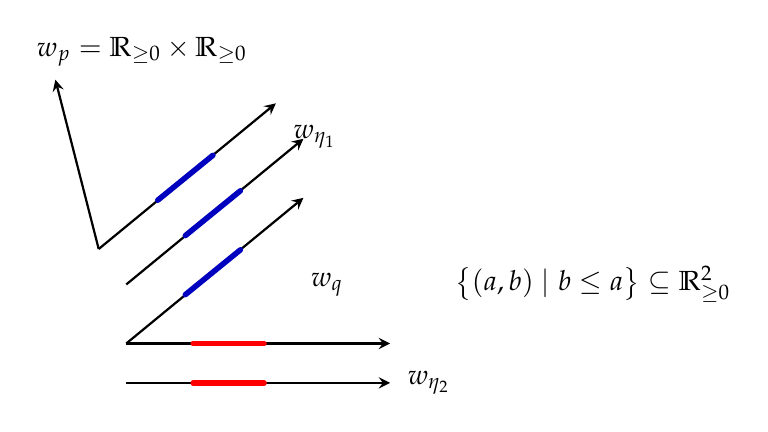
\begin{tikzpicture}[
        x=1cm,
        y=1cm,
        cone ray/.style={thick,->,>=stealth},
        common face/.style={red,line width=2pt,line cap=round},
        diagonal face/.style={blue!75!black,line width=2pt,line cap=round}
    ]
        % The cone at the marked point.
        \coordinate (p) at (0,4.45);
        \draw[cone ray] (p) -- ++(-0.55,2.15);
        \draw[cone ray] (p) -- ++(2.25,1.85);
        \draw[diagonal face]
            ($(p)+(0.75,0.62)$) -- ($(p)+(1.45,1.19)$);
        \node[above] at ($(p)+(0.55,2.2)$)
            {$w_p=\R_{\geq 0}\times\R_{\geq 0}$};

        % The cone at the first generic point.
        \coordinate (etaone) at (0.35,4);
        \draw[cone ray] (etaone) -- ++(2.25,1.85);
        \draw[diagonal face]
            ($(etaone)+(0.75,0.62)$) -- ($(etaone)+(1.45,1.19)$);
        \node[above right] at ($(etaone)+(2.0,1.6)$) {$w_{\eta_1}$};

        % The cone at the node.
        \coordinate (q) at (0.35,3.25);
        \draw[cone ray] (q) -- ++(2.25,1.85);
        \draw[cone ray] (q) -- ++(3.35,0);
        \draw[diagonal face]
            ($(q)+(0.75,0.62)$) -- ($(q)+(1.45,1.19)$);
        \draw[common face] ($(q)+(0.85,0)$) -- ($(q)+(1.75,0)$);
        \node at ($(q)+(2.55,0.75)$) {$w_q$};
        \node[anchor=west] at ($(q)+(4.05,0.75)$)
            {$\bigl\{(a,b)\mid b\leq a\bigr\}\subseteq\R_{\geq 0}^{2}$};

        % The colored intervals indicate the common faces used in the gluing.
        \coordinate (etatwo) at (0.35,2.75);
        \draw[cone ray] (etatwo) -- ++(3.35,0);
        \draw[common face] ($(etatwo)+(0.85,0)$) -- ($(etatwo)+(1.75,0)$);
        \node[right] at ($(etatwo)+(3.45,0)$) {$w_{\eta_2}$};
    \end{tikzpicture}
\end{figure}


\subsection{热带曲线}%
\label{sub:Tropical curves}

\begin{defn}
    锥 \(w, N_w\) 上的 \textit{热带曲线} 族 \((G, \vec{g}, \vec{\ell})\) 由如下数据组成
    \begin{enumerate}
        \item 连通图 \(G = V(G) \cup E(G) \cup L(G)\)；
        \item 腿的排序 \(\vec{m} \colon L(G) \xrightarrow{\sim} \ab\{1, \ldots, n\}\)；
        \item 亏格函数 \(\vec{g} \colon V(G) \to \N\)；
        \item 边长函数 \(\ell \colon E(G) \to \Hom(w \cap N_w, \N) \setminus \ab\{0\}\)。
    \end{enumerate}
\end{defn}

现在构造 \(\Sigma(G, \ell)\)。对 \(v \in V(G)\)，置 \(w_v = w\)。对 \(e \in E(G)\)，置
\[ w_e = \ab\{ (s, \lambda) \mid \lambda \leq \vec{\ell}(e)(s) \} \subseteq w \times \R_{\geq 0}. \]
对腿 \(\ell \in L(G)\)，置 \(w_{\ell} = w \times \R_{\geq 0}\)。现在需要定义面映射。若 \(\ell\) 与 \(v\) 关联，则面映射为
\[ w_v \hookrightarrow w_{\ell} \colon s \mapsto (s, 0). \]
若 \(e\) 与两个顶点 \(v_1, v_2\) 关联，则面映射为
\begin{align*}
    w_{v_1} \hookrightarrow w_e &\colon s \mapsto (s, \vec{\ell}(e)(s)) \\
    w_{v_2} \hookrightarrow w_e & \colon s \mapsto (s, 0).
\end{align*}
\begin{rmk}
    \(v_1\) 与 \(v_2\) 的选取不改变锥复形（在同构意义下），但在为对数映射定义接触阶时它确实有影响。然而一般而言，没有典范的方式来作此选取。
\end{rmk}

\subsection{穿孔曲线}%
\label{sub:Punctured curves}

穿孔对数曲线与穿孔映射发展于~\cite{ACGS2025}。

考虑结点曲线
\[ \Spec k[x,y]/xy \to \Spec k \]
其对数结构由 \(\N^2\) 给出，图表为 \((a,b) \mapsto x^a y^b\)，而 \(\N \to k\) 是标准对数点。现在考虑 \(\ul{C}_1 = Z(x) = \Spec k[y]\)，并以 \(p \colon \Spec k \to \Spec k[y]\) 标记该结点。注意
\[ C^{\on{can}} = (\ul{C}, M_C) \to S^{\on{can}} = \Spec(\N \to k). \]
记 \(M_{C_1}^{\circ} = M_C|_{C_1}\)。则在对数结构上有图表
\begin{equation*}
\begin{tikzcd}
    k[y] & & \N^2 \ar{ll}[swap]{(a,b) \mapsto 0^a y^b} \\
    k \ar{u} & & \N \ar{ll} \ar{u}{\Delta}.
\end{tikzcd}
\end{equation*}
特别地，可以计算茎 \(\bar{M}_{C_1}^{\circ}|_p = \N^2\)，因此有
\[ \bar{\pi}_{C_1^{\circ}}^{\flat} |_p \colon \N \xrightarrow{\Delta} \N^2. \]
然而本应有映射
\[ \bar{\pi}^{\flat}_{C_1}|_p \colon \N \xrightarrow{i_1} \N \oplus \N, \]
故 \(C_1\) \textbf{不是} 对数曲线。于是可以考虑图表
\begin{equation*}
\begin{tikzcd}
    \N \oplus \Z \\
    \N^2 \ar[hookrightarrow]{u} \ar{rr}{(0,1)\mapsto (0,1)}[swap]{(1,0)\mapsto (1,1)} & & \N^2 \ar{ull}[swap]{\Vectorstack{{(1,0)\mapsto(1,-1)} {(0,1)\mapsto(0,1)}}} \\
    & \N \ar{ul}{i_1} \ar{ur}{\Delta}.
\end{tikzcd}
\end{equation*}
因此我们将考虑扩张对数结构。

回顾对数曲线满足 \(M_{\mc{C}} = M_{\mc{C}}' \oplus_{\mc{O}_{\mc{C}}^{\times}} P_{\mc{C}}\)，其中 \(P_{\mc{C}}\) 是由标记给出的除子对数结构。

\begin{defn}
    fs 对数概形 \(S\) 上的 \textit{穿孔曲线} 由 \((\mc{C}^{\circ} \xrightarrow{p} \mc{C} \xrightarrow{\pi} S, \{p_i\}_{i=1}^n)\) 组成，其中 \((\mc{C} \xrightarrow{\pi} S, \vec{p})\) 是对数曲线，且映射 \(p \colon \mc{C}^{\circ} \to \mc{C}\) 是 fine 对数概形之间的映射，满足下列条件：
    \begin{enumerate}
        \item 底映射 \(\ul{p}\) 是同构；
        \item 在对数结构上，映射 \(p^{\flat} \colon M_{\mc{C}} \hookrightarrow M_{\mc{C}^{\circ}}\) 在 \(p_i\) 之外是同构，并诱导
            \[ M_{\mc{C}} \xrightarrow{p^{\flat}} M_{\mc{C}^{\circ}} \hookrightarrow M_{\mc{C}} \oplus P^{\mr{gp}}. \]
        \item 对任意标记 \(p_i\) 及任意 \(s \in M_{\mc{C}^{\circ}, p_i} \setminus M_{\mc{C}, p_i}\)，有 \(\alpha_{\mc{C}^{\circ}}(s) = 0\)。
    \end{enumerate}
\end{defn}

粗略地说，穿孔曲线就是对数曲线加上一个交换图表
\begin{equation*}
\begin{tikzcd}
    M_{\mc{C}^{\circ}} \ar{dr} \ar[hookrightarrow]{r} & M_{\mc{C}}' \oplus_{\mc{O}_{\mc{C}}^{\times}} P^{\on{gp}} \\
    & \mc{O}_{\mc{C}} \\
    M_{\mc{C}} \ar[hookrightarrow]{uu} \ar{ur}.
\end{tikzcd}
\end{equation*}


\begin{exm}
    设 \((\ul{\mc{C}} \to \ul{S} = \Spec k, p)\) 是光滑的 \(1\)-点曲线。
    \begin{enumerate}
        \item 设 \((\mc{C}/S, p)\) 赋予典范对数结构（即 \(S\) 无对数结构）。令 \(M_{\mc{C}} = P\)。则任何穿孔 \(p^{\flat} \colon M_{\mc{C}} \hookrightarrow M_{\mc{C}^{\circ}} \subset P^{\on{gp}}\) 必为平凡。原因在于 \(M_{\mc{C}^{\circ}}\) 不能有截面 \(s\) 使得 \(\alpha_{\mc{C}^{\circ}}(s) = 0\)。若 \(s \in P = M_{\mc{C}}\)，则 \(\alpha_{\mc{C}^{\circ}}(s) = \alpha_{\mc{C}}(s)\)。否则若 \(s \notin P\)，则因 \(\alpha_{\mc{C}^{\circ}}(-s)\) 非零，\(\alpha_{\mc{C}^{\circ}}(s)\) 也非零。
        \item 设 \(M_{\mc{C}^{\circ}} \subseteq (\N \oplus \mc{O}_{\mc{C}}^{\times}) \oplus P^{\on{gp}}\) 是一个穿孔。取 \(\mc{O}(-p)\) 的一个局部生成元 \(x\)。则任意 \(s \in M_{\mc{C}^{\circ}, p}\) 具有形式 \(s = ((n, \varphi), x^m)\)，其中 \(n \in \N\)，\(\varphi \in \mc{O}_{\mc{C}, p}^{\times}\)。若 \(m < 0\)，则我们要求 \(\alpha_{\mc{C}^{\circ}}(s) = 0\)。这意味着 \(\alpha_{\mc{C}}((n, \varphi), 0) = 0\)，因此
            \[ \bar{M}_{\mc{C}^{\circ}, p} \subseteq \ab\{(n, m) \in \N \oplus \Z \mid m \geq 0 \text{ if } n = 0 \}. \]
            事实上，右端任意包含 \(\N \oplus \N\) 的 fine 子幺半群均可由某个穿孔实现。
        \item 设 \(S = \Spec(\N \to k)\)。考虑 \(M_{\mc{C}^{\circ}}\) 使得 \(\bar{M}_{\mc{C}^{\circ}, p} = \N^2 + \N (2,-2)\)。由于 \((1,-1) \notin \bar{M}_{\mc{C}^{\circ}, p}\)，可见 \(M_{\mc{C}^{\circ}}\) 不是饱和的。
    \end{enumerate}
\end{exm}

\begin{lem}[{\cite{ACGS2025}}]
    设 \(Q\) 是尖的 fs 幺半群。令 \(w \coloneqq \Hom(Q, \R_{\geq 0}) = Q_{\R}^{\vee}\)。设 \(Q^{\circ} \subseteq Q \oplus \Z\) 有限生成，且 \(Q \oplus \N \subsetneq Q^{\circ}\) 以及 \(Q^{\circ} \cap \ab\{0\} \times \Z_{<0} = \emptyset\)。则存在非零的凹的分段线性函数
    \[ \ell \colon w \to \R_{\geq 0} \]
    具有有理斜率，使得
    \[ (Q^{\circ})_{\R}^{\vee} = \ab\{ (s, \lambda) \in w \times \R_{\geq 0} \mid 0 \leq \lambda \leq \ell(s) \}. \]
\end{lem}

\begin{exm}
    设 \(Q = \N^2\)，置
    \begin{align*}
        Q^{\circ} &= \ab<((1,0), -1), ((0,1), -1), ((0,0),1)> \subset \N^2 \oplus \Z \\
        &= \ab\{((a,b), m) \mid a+b+m \geq 0, a,b \geq 0 \}.
    \end{align*}
    则
    \[ (Q^{\circ})_{\R}^{\vee} = \ab\{ (e_x, e_y, e_t) \mid 0 \leq e_t \leq \min(e_x, e_y) \}. \]
\end{exm}






\section{兼顾高亏格的 GW 理论导论（Patrick Lei）}%
\label{sec:Intro to GW theory with a view to higher genus (Patrick Lei)}


\subsection{GW 理论简介}%
\label{sub:Introduction to GW theory}

关于虚基本类的构造，参见~\cite{BehrendFantechi1997}；关于公理与量子上同调，参见~\cite{KM1994}。

这些讲座的目标是以一种便于进行高亏格计算的方式讨论格罗莫夫–威滕理论。格罗莫夫–威滕理论研究模空间 \(\Mbar_{g,n}(X, \beta)\) 上的积分，其中 \(X\) 是光滑射影代数簇，\(\beta \in H_2(X, \Z)\) 是有效曲线类。有如下图表
\begin{equation*}
\begin{tikzcd}
    \mc{C} \ar{r}{f} \ar[bend right=20]{d}[swap]{\pi} & X \\
    \Mbar_{g,n}(X, \beta) \ar[bend right=20]{u}[swap]{\sigma_i} \ar{ur}[swap]{\on{ev}_i}
\end{tikzcd}
\end{equation*}
其中 \(\mc{C}\) 是万有曲线，\(\sigma_i\) 是给出标记点的 \(\pi\) 的截面，\(f\) 是万有稳定映射，\(\ev_i = f \circ \sigma_i\) 是求值态射。尽管 \(\Mbar_{g,n}(X, \beta)\) 一般是奇异的、非等维的且可约的，但存在一个特殊的类
\[ [\Mbar_{g,n}(X, \beta)]^{\vir} \in A_{\ab(c_1(X), \beta) + (\dim X - 3)(1-g) + n}(\Mbar_{g,n}(X, \beta), \Q), \]
它称为\textit{虚基本类}。

\begin{exer}
    利用形变理论中的标准论证，验证 \(\Mbar_{g,n}(X, \beta)\) 的“期望维数”就是上面给出的数。
\end{exer}

在 \(X\) 光滑射影的假设下，\(\Mbar_{g,n}(X, \beta)\) 是真（proper）的，故可定义\textit{GW 不变量}
\[ \ab<\tau_{a_1}(\alpha_1), \cdots, \tau_{a_n}(\alpha_n)>_{g,n,\beta} \coloneqq \int_{[\Mbar_{g,n}(X, \beta)]^{\vir}} \prod_{i=1}^n \ev_i^* \alpha_i \cdot \psi_i^{a_i} \]
其中 \(\alpha_i \in H^*(X)\)。这里 \(\psi_i\) 由 \(\psi_i = c_1(\sigma_i^*(\omega_{\pi}))\) 定义。

遗憾的是，计算单个格罗莫夫–威滕不变量非常困难，因此我们转而考虑更为困难的问题：研究 GW 不变量的生成级数，例如当 \(X\) 为卡拉比–丘三维簇时的
\[ F_g = \sum_{\beta \geq 0} q^{\beta} \ab<>_{g,0,\beta} \]
这里 \(q\) 是记录曲线类的形式变量，我们将环 \(\Q\ps{q^{\beta} \mid \beta \in H_2(X, \Z)_{\mr{eff}}}\) 记作 \(\Lambda\)。我们还要考虑一些其他结构。首先可以考虑\textit{量子上同调环}，其乘积 \(a \star_{\mbf{t}} b\) 由下式给出
\[
    (a \star_{\mbf{t}} b, c) = \sum_{\substack{\beta \geq 0 \\ n \geq 0}} \ab<a,b,c, \mbf{t}, \ldots, \mbf{t}>_{0,3+n,\beta} \frac{q^{\beta}}{n!}.
\]
这里 \(a,b,c, \mbf{t} \in H^*(X)\)。我们还要考虑\textit{量子联络}。设 \(\ab\{ e_i \}\) 是 \(H^*(X)\) 的一组基。则量子联络是平凡丛上的联络，其纤维为 \(H^*(X)\)，底空间为 \(H^*(X) \times \P^1_z\)，由下式给出
\[ \nabla_{t^i} = \partial_{t^i} + \frac{1}{z} e_i \star_{\mbf{t}}. \]
有时考虑 \(z\) 方向上的联络也很有用，它由下式给出
\[ \nabla_{z \odv{}{z}} \coloneqq z \odv{}{z} - \frac{1}{z} E_X \star_{\mbf{t}} + \mu_X, \]
其中 \(\mu_X(\alpha) = \frac{\deg(\alpha) - \dim X}{2} \alpha\) 是分次算子，而
\[ E_X = c_1(X) + \sum_i \ab(1 - \frac{\deg(e_i)}{2})t^i e_i \]
是\textit{欧拉向量场}。由于我们主要关注卡拉比–丘簇，故不再考虑它。

\subsection{亏格零的枚举镜像对称}%
\label{sub:Enumerative mirror symmetry in genus zero}

数学家发展并研究格罗莫夫–威滕理论的动力来自 20 世纪 90 年代初：当时 Candelas、de la Ossa、Green 与 Parkes~\cite{CandelasEtAl1991} 通过把问题转化为计算另一个称为\textit{镜像五次三维簇}的卡拉比–丘三维簇上的周期积分（等价地，研究其霍奇结构的变分），预言了一般五次三维簇上低次数有理曲线的数目。在亏格零时，所有不变量均可由\textit{J-函数} \(J_{\mbf{t}}(q,z) \in H^*(X, \Lambda)[z]\) 恢复，其定义为
\[ \ab( J_{\mbf{t}}(q, z), \alpha ) \coloneqq (z + \mbf{t}, \alpha) + \sum_{n, \beta} \frac{q^{\beta}}{n!} \ab< \frac{\alpha}{z-\psi}, \mbf{t}, \ldots, \mbf{t}>_{0,1+n, \beta} \]
其中 \(\mbf{t} \in H^*(X, \Lambda)[z]\)，\(\alpha \in H^*(X)\)，而 \((-,-)\) 是庞加莱配对。因此，计算所有带后代（即 \(\psi\)-类）的亏格零格罗莫夫–威滕不变量的问题，归结为计算 J-函数。

\begin{rmk}
    我们将 \(\frac{1}{z-\psi}\) 展开为 \(\sum_{k=0}^{\infty} \psi^k z^{-k-1}\)。  
\end{rmk}

我们应当指出，J-函数可以通过量子微分方程的基本解得到，该基本解由下式给出
\[ ( S_{\mbf{t}}(z) \phi , \alpha) = (\phi, \alpha) + \sum_{n, \beta} \frac{q^{\beta}}{n!} \ab<\frac{\alpha}{z-\psi}, \phi, \mbf{t}, \ldots, \mbf{t}>_{0, 2+n, \beta}. \]
它具有性质 \(S_{\mbf{t}}^*(-z) S_{\mbf{t}}(z) = \on{Id}\)，这通常称为\textit{辛性质}。由此我们可由 \(z S_{\mbf{t}}^*(z)\cdot 1 = J_{\mbf{t}}(q, z)\) 恢复 J-函数。

在物理学中，镜像对称是称为 A 模型与 B 模型的两种理论之间的对偶，因此现在我们需要引入 B 模型的对象。为节省时间（并简化记号），我们假设 \(X\) 是环面簇且 \(-K_X\) 数值有效（nef）。设 \(D_1, \ldots, D_r\) 为 \(X\) 中全部的环面不变除子。定义\textit{\(I\)-函数}如下
\[
    I_{\mbf{t}}(q, z) \coloneqq z e^{\mbf{t}/z} \sum_{\beta \geq 0} q^{\beta} \frac{\prod_{i=1}^r \prod_{m = -\infty}^{0} (D_i + mz)}{\prod_{i=1}^r \prod_{m=-\infty}^{\beta \cdot D_i} (D_i + mz)}.
\]
注意，此处我们将出现的任意 \((D_i + mz)^{-1}\) 展开为 \(\frac{1}{mz} \ab(1 - \frac{D_i}{mz} + \cdots)\)，即展开为 \(\frac{D_i}{mz}\) 的几何级数。此外，I-函数被一个称为\textit{Picard–Fuchs 方程}的微分方程所零化，它是某种超几何型方程。

\begin{exm}
    若 \(\mbf{t} = 0\) 且 \(X = \P^1\)，则得到
    \begin{align*}
        I(q,z) &= z\sum_{d \geq 0} q^d \frac{1}{\prod_{m=1}^d (H + mz)^2} \\
        &= z\sum_{d \geq 0} \ab(\frac{q}{z^2})^d \frac{1}{(d!^2)} + O(H),
    \end{align*}
    于是实际上我们看到首项为第一类贝塞尔函数。
\end{exm}

若 \(X\) 是环面簇 \(Y\) 中由线丛 \(L_1, \ldots, L_k\) 切出的完全交，且这些线丛都满足 \(H^1(f^* L_i) = 0\)（对任意到 \(Y\) 的亏格零稳定映射成立，这称为\textit{凸}的），则量子 Lefschetz 定理~\cite{CoatesGivental2007} 允许我们把 \([\Mbar_{g,n}(X, \beta)]^{\vir}\) 替换为 \(e\ab(\bigoplus \pi_* f^* L_i) \cap [\Mbar_{g,n}(Y, \beta)]^{\vir}\)，并在 \(Y\) 上进行所有计算。此时 I-函数定义为
\[
    I_{\mbf{t}}(q,z) \coloneqq z e^{\mbf{t}/z} \sum_{\beta \geq 0} q^{\beta} \frac{\prod_{i=1}^k \prod_{m=-\infty}^{L_i \cdot \beta} (L_i + mz)}{\prod_{i=1}^k \prod_{m=-\infty}^{0} (L_i + mz)} \frac{\prod_{i=1}^r \prod_{m = -\infty}^{0} (D_i + mz)}{\prod_{i=1}^r \prod_{m=-\infty}^{\beta \cdot D_i} (D_i + mz)},
\]
其中我们滥用记号，将 \(L_i\) 与其第一陈类混同。

\begin{exm}
    对于由 \(\mc{O}_{\P^4}(5)\) 的一个截面切出的五次三维簇，\(\mbf{t} = 0\) 处的 I-函数为
    \[ I(q,z) = z \sum_{d \geq 0} q^d \frac{\prod_{m=1}^{5d}(5H+mz)}{\prod_{m=1}^d (H+mz)^5}. \]
\end{exm}

亏格零镜像定理的内容是这两个对象之间的对应。更精确地说，在 \(-K_X\) 数值有效的情形下，它们通过变量变换相联系。

\begin{thm}[{\cite{Givental1998,LLY1997}}]
    将 \(\mbf{t} = 0\) 的 I-函数写成 \(I_0(q) \cdot z + I_1(q) + O(z^{-1})\)。则有
    \[
        J_{\tau(\mbf{t})}(q,z) = \frac{I_{\mbf{t}}(q,z)}{I_0(q)},
    \]
    其中 \(\tau(\mbf{t}) = \frac{\mbf{t} + I_1(q)}{I_0(q)}\)。
\end{thm}

\begin{exm}
    当 \(X = \P^1\) 时，注意到 \(I_0(q) = 1\) 且 \(I_1(q) = 0\)，故实际上我们有等式
    \[ J_{\mbf{t}}(q,z) = I_{\mbf{t}}(q,z). \]
\end{exm}

\begin{exm}
    当 \(X\) 为五次三维簇时，为方便起见，我们将 I-函数的各分量改写为 \(I_0(q) \cdot z + I_1(q)H + O(z^{-1})\)。我们有
    \[ I_0(q) = \sum_{d \geq 0} \frac{(5d)!}{(d!)^5} q^d, \qquad I_1(q) = \sum_{d \geq 0} \frac{(5d)!}{(d!)^5} \ab(5\sum_{m=d+1}^{5d} \frac{1}{m}) q^d, \]
    故此情形下镜像映射非平凡。取 \(\mbf{t} = 0\)，我们看到 \(\tau = \frac{I_1(q)H}{I_0(q)}\)，于是得到
    \[ J_{\tau}(q,z) = \frac{I(q,z)}{I_0(q)}. \]
    由除子方程，左边也等于 \(J(qe^{I_1/I_0}, z)\)，我们也称之为镜像映射。
    因此，我们可以用镜像定理计算 $\star_{\tau}$。\(H^2\) 方向上的量子联络化为常微分方程
    \[ (H+zD) S_{\tau}(z)^* = S_{\tau}(z)^* \cdot I_{11} H \star_{\tau}, \]
    其中 $D \coloneqq q \odv{}{q}$（这里坐标为 $\log q$），$I_{11} \coloneqq 1 + D \ab(\frac{I_1(q)}{I_0(q)})$。利用镜像定理及 Zagier--Zinger~\cite{ZagierZinger2008} 的结果进行显式计算可得
    \begin{align*}
        I_{11} H + \cdots &= S_{\tau}(z)^* (I_{11} H \star_{\tau} \1) \\
        \ab( 1 + D\ab(\frac{\frac{I_1}{I_0} + D \ab(\frac{I_2}{I_0})}{I_{11}}) ) H^2 + \cdots &= S_{\tau}(z)^* (I_{11} H \star_{\tau} H) \\
        I_{11} H^3 &= S_{\tau}(z)^* (I_{11}H \star_{\tau} H^2).
    \end{align*}
    由于 $S_{\tau}$ 以恒同映射起首，这就计算出了 $H \star_{\tau}$。
\end{exm}

\subsubsection{振荡积分}%
\label{ssub:Oscillating integrals}

现在我们重新解释亏格零镜像定理；在讨论高亏格不变量时将回到这一解释。特别地，我们将把 I-函数解释为 \(X\) 的某个镜像族上的积分，对我们而言该镜像族是环面簇。设
\[ 0 \to \Lambda \to \Z^r \to N \to 0 \]
为 \(X\) 的扇序列。施加 \(\Hom(-, \C^{\times})\)，得到正合列
\[ 1 \to (\C^{\times})^{\dim X} \to (\C^{\times})^r \to \Hom(\Lambda, \C^{\times}) \to 1. \]
设映射 \(\Lambda \to \Z^r\) 由矩阵 \((m_{ij})_{i=1,\ldots,r}^{j = 1, \ldots, \rho(X)}\) 给出。考虑与 \(X\) 镜像的簇
\[ E_q = \ab(\prod_{i=1}^r x_j^{m_{ij}} = q_i \middle\vert i=1, \ldots, \rho(X)) \]
并考虑超势 \(f = x_1 + \cdots + x_r\)。若希望考虑等变理论，其中等变参数 \(\lambda_1, \ldots, \lambda_r\) 作用于 \(X\) 的各个齐次坐标，则考虑 \(f_{\lambda} = \sum_{i=1}^r (x_i - \lambda_i \log x_i)\)。

\begin{exm}
    当 \(X = \P^n\) 时，\(X\) 的镜像是超势 \(\sum_{i=1}^{n+1} (x_i - \lambda_i \log x_i)\)，定义在簇 \(E_q = (x_1 \cdots x_{n+1} = q)\) 上。
\end{exm}

现在我们选取合适的 Lefschetz 闭链 \(\Gamma_{\alpha}\)，位于（等变）超势的每个临界点 \((x_{\alpha})\) 附近，并考虑积分
\[ I_{\alpha} = \int_{\Gamma_{\alpha}} e^{f_{\lambda}/z} \prod_{i=1}^r \frac{\d{x_i}}{x_i}. \]
在 I-函数方面，这相当于将表达式中的每个 \(D_i\) 替换为 \(D_i - \lambda_i\)（即打开等变参数）；在 J-函数方面，则相当于考虑 \(X\) 的完全等变 GW 理论。在亏格零时，\(\lambda_i \to 0\) 的极限存在，因此我们可以放心地由下述结果恢复原来的镜像定理：

\begin{thm}[{\cite{Givental1996}}]
    该积分被与 I-函数相同的 Picard–Fuchs 方程所零化，且除各种前因子外，它沿负实轴 \(z \to 0^-\) 时的渐近展开与 I-函数在 \(X\) 上对应于临界点 \(( x_{\alpha} )\) 的 T-不动点处的限制一致。
\end{thm}


\subsubsection{拉格朗日锥}%
\label{ssub:The Lagrangian cone}

\(X\) 的量子上同调是\textit{弗罗贝尼乌斯流形}的一个例子；稍后我们将看到，任何上同调场论都能给出这样的流形。记 \(V = H^*(X)\)，设 \((e_{\mu})\) 为 \(V\) 的一组基，于是可写 $\bv = \sum_{\mu,n} t^{\mu}_n e_{\mu} z^n \in V\ps{z}$。
弗罗贝尼乌斯流形的结构来自函数
\[
    \mc{F}_0(\bv) = \sum_{n, \beta, \mu} \frac{q^{\beta}}{n!} \ab<\bv(\psi), \ldots, \bv(\psi)>_{0,n,\beta},
\]
它也称为 \(X\) 的\textit{亏格零后代势}。它满足弦方程、膨胀子方程以及拓扑递归关系：
\begin{align*}
    \pdv{}{t_0^1} \mc{F}_0 &= \frac{1}{2} (\bv_0, \bv_0) + \sum_{n=0}^{\infty} \sum_{\mu} t_{n+1}^{\mu} \pdv{}{t_n^{\mu}} \mc{F}_0; \\
    \pdv{}{t_1^1} \mc{F}_0 &= \sum_{n=0}^{\infty} \sum_{\mu} t_n^{\mu} \pdv{}{t_n^{\mu}}\mc{F}_0 - 2 \mc{F}_0; \\
    \pdv{}{t_{k+1}^{\alpha},t_m^{\beta},t_n^{\gamma}} \mc{F}_0 &= \sum_{\mu,\nu} \pdv{}{t_k^{\alpha},t_0^{\mu}} \mc{F}_0 \cdot \eta^{\mu\nu} \cdot \pdv{}{t_0^{\nu},t_{m}^{\beta},t_n^{\gamma}} \mc{F}_0.
\end{align*}
为叙述下述结果，考虑带辛形式
\[ \omega(\mbf{f}(z), \mbf{g}(z)) \coloneqq \on{Res}_{z=0}(\mbf{f}(-z), \mbf{g}(z)). \]
的无穷维向量空间 $V\ls{z^{-1}}$（或其某个完备化）。我们还考虑新变量\footnote{这称为\textit{膨胀子平移}。} $\bq = \bv - z$，于是 $\mc{F}_0$ 现在是 $\bq = -z$ 附近的函数。

\begin{thm}[Givental {\cite{Givental2004}}]
    $\mc{F}_0$ 满足上述偏微分方程组，当且仅当 $\mc{L}$（即 $\d{\mc{F}_0}$ 的图像）是顶点位于 $\bq = 0$ 的拉格朗日锥，且其切空间 $L$ 与 $\mc{L}$ 恰好沿 $zL \subset L$ 相切。
\end{thm}

我们可以通过以下步骤恢复拉格朗日锥 $\mc{L}$。先求量子联络的一个基本解
\[ S = \mr{Id} + S_1 z^{-1} + S_2 z^{-2} + \cdots \]
它满足方程
\[ z \pdv{}{t^{\mu}}S = e_{\mu} \star S. \]
然后令 $J \coloneqq z S^*(z) \1$，即可按以下步骤恢复拉格朗日锥：
\begin{itemize}
    \item 导数 $\pdv{}{t^{\mu}} J$ 构成 $L \cap V\ps{z^{-1}}$ 的一组基；
    \item 这意味着 $z \pdv{}{t^{\mu},t^{\nu}} J \in L \cap V \ps{z^{-1}}$。将它们用一阶导数表出，并利用 $J$ 求解量子联络这一事实，我们恢复弗罗贝尼乌斯结构，从而恢复拉格朗日锥。
\end{itemize}

由此，我们可以将亏格零镜像定理解释为：
\begin{thm}[{\cite{Givental1998}}]
    I-函数 \(I_{\mbf{t}}(q,z)\) 位于 \(X\) 的拉格朗日锥上。
\end{thm}




\subsection{曲线模空间与上同调场论}%
\label{sub:Moduli of curves and CohFTs}

上同调场论的概念由 Kontsevich--Manin~\cite{KM1994} 引入。

我们用 $\Mbar_{g,n}$ 记亏格 $g$、带 $n$ 个标记点的稳定曲线的模空间。它非空当且仅当 $2g-2+n > 0$，此时它是维数为 $3g-3+n$ 的 Deligne–Mumford 叠。族 $\Mbar_{g,n}$ 具有组合结构，它由一族态射给出。
\begin{itemize}
    \item 存在粘合态射
        \[q \colon \Mbar_{g,n+1} \times \Mbar_{h, m+1} \to \Mbar_{g+h,n+m}, \]
        它取两条曲线并沿最后一个标记点将它们粘合以形成一个结点；
    \item 存在自粘合态射 \[s \colon \Mbar_{g-1,n+2} \to \Mbar_{g,n},\]
        它粘合最后两个标记点。
\end{itemize}
当然还有另一个有趣的映射，即遗忘映射
\[ \pr \colon \Mbar_{g,n+1} \to \Mbar_{g,n} \]
它删除最后一个标记点然后再作稳定化。现在我们可以定义我们感兴趣的枚举理论，其中包括格罗莫夫–威滕理论。

\begin{defn}
    给定向量空间 $V$，其上带非退化对称双线性型 $\eta$ 及单位元 $\1 \in V$，一个\textit{上同调场论（CohFT）} $\Omega$ 是指 $V$ 上的一族映射 $\Omega_{g,n}$，其中每个都是 $S_n$-等变线性映射
    \[ \Omega_{g,n} \colon V^{\otimes n} \to H^*(\Mbar_{g,n}) \]
    满足基本恒等式
    \[ \Omega_{0,3}(\1, u,v) = \eta(u,v) \]
    及以下组合恒等式（取 $e_{\mu}$ 为 $V$ 的基，使得 $e_1 = \1$，$e^{\mu}$ 为对偶基）：
    \begin{align*}
        q^* \Omega_{g+h,n+m}(\bv_1, \bv_2) &= \sum_{\mu} \Omega_{g,n+1}(\bv_1, e_{\mu}) \cdot \Omega_{h,m+1}(  \bv_2, e^{\mu} ); \\
        s^* \Omega_{g,n}(\bv) &= \sum_{\mu} \Omega_{g,n+2}(\bv, e_{\mu}, e^{\mu}).
    \end{align*}
    若此外还满足恒等式
    \[ \pr^*\Omega_{g,n}(\bv) = \Omega_{g,n+1}(\bv,\1) \]
    则称该 CohFT 具有\textit{平坦单位}（或满足\textit{弦方程}）。
\end{defn}
以上均可推广到超向量空间，但为简单起见我们不处理这种情形。

\begin{exm}
    CohFT 最重要的例子是光滑射影簇 $X$ 的格罗莫夫–威滕理论。这里回顾一下，稳定映射的源是一条 \textbf{预稳定}曲线，因此存在稳定化态射
    \[ \st \colon \Mbar_{g,n}(X,\beta) \to \Mbar_{g,n} \]
    它遗忘映射并对曲线作稳定化。于是在 Novikov 环上工作，取 $V = H^*(X)$，$\eta$ 为庞加莱配对，$\1$ 为 $X$ 的基本类。线性映射 $\Omega^X_{g,n}$ 由下式给出
    \[ \Omega_{g,n}^X(\btau) \coloneqq \sum_{\beta} q^{\beta} \st_* \ab(\prod_{i=1}^n \ev_i^*(\tau_i) \cap [\Mbar_{g,n}(X,\beta)]^{\vir}), \]
    其中 $\ev_i \colon \Mbar_{g,n}(X,\beta) \to X$ 是第 $i$ 个求值映射。
\end{exm}

\begin{exm}
    设 $\pi \colon \mc{C}_{g,n} \to \Mbar_{g,n}$ 为万有曲线。则\textit{霍奇丛}是向量丛
    \[ \E_{g,n} \coloneqq \pi_* \omega_{\pi}. \]
    再考虑带通常配对的向量空间 $V = \C$，并按下式定义 CohFT $\Omega^{\E}$：
    \[ \Omega^{\E}_{g,n} \coloneqq c(\E_{g,n}). \]
    粘合公理由等式 $q^* \E_{g+h} = \E_g \oplus \E_h$ 与正合列
    \[ 0 \to \E_{g-1} \to \E_g \to \mc{O} \to 0. \]
    满足。这里由于亏格零分支对 $\omega$ 的整体截面没有贡献，且 $\E$ 不依赖于标记点，该 CohFT 具有平坦单位。
\end{exm}

\begin{rmk}
    稍后我们将看到，由量子黎曼–罗赫定理，这与一点的 GW CohFT 相关。
\end{rmk}

给定 CohFT $\Omega$，将类 $\Omega_{g,n}(\bv)$ 与 $\Mbar_{g,n}$ 上的各种上同调配对即可得到不变量。其中最值得考虑的是类
\[ \bar{\psi}_i \coloneqq c_1( s_i^* \omega_{\pi} ), \]
这里 $s_i \colon \Mbar_{g,n} \to \mc{C}_{g,n}$ 是第 $i$ 个标记点。

\begin{rmk}
    在格罗莫夫–威滕理论中，这些称为\textit{先祖}。还有后代，它由同样的公式给出，只是用预稳定曲线的模空间 $\mf{M}_{g,n}$ 代替 $\Mbar_{g,n}$，其中我们将上面定义的态射 $\st$ 分解为
    \[ \Mbar_{g,n}(X,\beta) \xrightarrow{\text{forget map}} \mf{M}_{g,n} \xrightarrow{\text{stabilize}} \Mbar_{g,n}. \]
    后代类记作 $\psi_i$。
\end{rmk}

\begin{exm}
    我们将计算一个将在卡拉比–丘三维簇的 GW 理论中出现的不变量。对任意 CohFT $\Omega$，考虑不变量
    \[ \ab<\1\bar{\psi}_1>_{1,1}^{\Omega}\coloneqq \int_{\Mbar_{1,1}} \Omega_{1,1}(\1)\bar{\psi}_1. \]
    利用第二个粘合方程，$\Omega_{1,1}(\1)$ 的零次部分等于
    \[ \sum_{\mu} \Omega_{0,3}(\1, e_{\mu}, e^{\mu}) = \sum_{\mu} \eta(e_{\mu}, e^{\mu}), \]
    这给出（分次）维数 $\chi(V)$，也就是 $V$ 的（分次）维数（例如，若 \(V = H^*(X)\)，其中 \(X\) 为卡拉比–丘三维簇，则这是 \(X\) 的拓扑欧拉示性数）。于是我们得到
    \[ \ab<\1\bar{\psi}_1>_{1,1}^{\Omega} = \frac{\dim V}{24}. \]
\end{exm}

\begin{exm}
    考虑一点的 GW CohFT。它由带通常配对的 $V = \C$ 及公式
    \[ \Omega_{g,n} = 1. \]
    给出。于是我们定义不变量
    \[ \ab<\bar{\psi}_1^{a_1} \cdots \bar{\psi}_n^{a_n}>_{g,n} \coloneqq \int_{\Mbar_{g,n}} \Omega_{g,n} \cdot \bar{\psi}_1^{a_1} \cdots \bar{\psi}_n^{a_n}. \]
    \begin{thm}[Kontsevich {\cite{Kontsevich1992}}]
        函数
        \[ \mc{D} \coloneqq \exp \ab(\sum_{g,n} \frac{\hbar^{g-1}}{n!}\sum_{a_1 + \cdots + a_n = 3g-3+n} \ab<\bar{\psi}_1^{a_1} \cdots \bar{\psi}_n^{a_n}>_{g,n} t_{a_1}\cdots t_{a_n}) \]
        被以下算子零化：
        \begin{align*}
            L_{-1} \coloneqq{}& -\pdv{}{t_0} + \frac{\hbar^{-1}}{2} t_0^2 + \sum_{i=0}^{\infty} t_{i+1} \pdv{}{t_i};\\
            L_0 \coloneqq{}& -\frac{3}{2} \pdv{}{t_1} + \sum_{i=0}^{\infty} \frac{2i+1}{2} t_i \pdv{}{t_i} + \frac{1}{16};\\
            L_n \coloneqq{}& -\frac{(2n+3)!!}{2^{n+1}} \pdv{}{t_{n+1}} + \sum_{i=0}^{\infty} \frac{(2i+2n+1)!!}{(2i-1)!! 2^{n+1}} t_i \pdv{}{t_{i+n}} \\
            &+ \frac{\hbar}{2} \sum_{i=0}^{n-1} \frac{(2i+1) (2i-1) \cdots (2i+1-2n)}{2^{n+1}} \pdv{}{t_i,t_{n-1-i}}.
        \end{align*}
    \end{thm}
\end{exm}

\begin{rmk}
    这一结果（一点的 Virasoro 约束）等价于 $\mc{D}$ 是 KdV 族的 \(\tau\)-函数，并已被多位作者推广。
\end{rmk}




\subsection{\(R\)-矩阵作用}%
\label{sub:R-matrix action}

21 世纪初，Givental 发现了公理化枚举理论的一个显著性质，即可以利用满足如下性质的矩阵 $R(z) = R_0 + R_1 z + R_2 z^2 + \cdots \in \Hom(V, V')\ps{z}$ 的作用来变换 CohFT
\[ R^*(-z) R(z) = \mr{Id}_V. \]
传统上，文献要求 $V = V'$ 且 $R_0 = \mr{Id}$，但 MSP 群已经去除了这一限制，并且也允许 $\dim V < \dim V'$。

为了定义 $R$ 在 $V$ 上的 CohFT $\Omega$ 上的作用，我们需要回顾 $\Mbar_{g,n}$ 的一些组合结构。对曲线 $C\in \Mbar_{g,n}(\C)$，可以考虑 $C$ 的对偶图，它由顶点、边和腿（leg）组成，定义如下：
\begin{itemize}
    \item 顶点对应于 $C$ 的不可约分支，并由一个非负整数标记，即其亏格；
    \item 边对应于 $C$ 的结点（特别地，我们允许环）；
    \item 腿对应于标记点。
\end{itemize}
任何作为稳定曲线的对偶图出现的图都称为 \textit{稳定图}。

\begin{figure}[htpb]
  \centering
  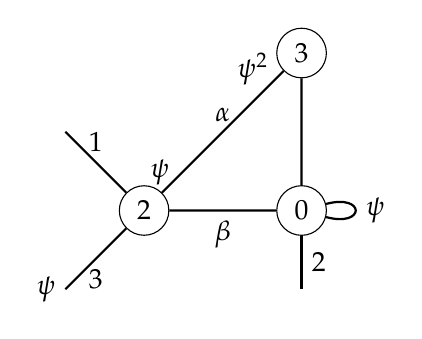
\begin{tikzpicture}[scale=1,transform shape,every loop/.style={}]
    \node[circle,draw] (A) at (0,0) {$2$};
    \node[circle,draw] (B) at (2,2) {$3$};
    \node[circle,draw] (C) at (2,0) {$0$};
    \draw[thick] (A) -- node[above]{$\alpha$} (B) -- (C) -- node[below]{$\beta$} (A);
    \draw[thick] (A) -- node[below]{$3$} (-1,-1);
    \draw[thick] (A) -- node[above]{$1$} (-1,1);
    \draw[thick] (C) -- node[right]{$2$} (2,-1);
    \draw[thick] (C) edge[loop right] node[right] {$\psi$} (C);
    \node[anchor=east] at (-1,-1) {$\psi$};
    \node[anchor=east] at (1.7,1.8) {$\psi^2$};
    \node[anchor=south] at (0.2,0.2) {$\psi$};
  \end{tikzpicture}
  \caption{$\ol{\mc{M}}_{7,3}$ 中的一个稳定图及其相伴重言类。该稳定图描述了映射
    $\ol{\mc{M}}_{2,4} \times \ol{\mc{M}}_{3,2} \times \ol{\mc{M}}_{0,5} \to \ol{\mc{M}}_{7,3}$ 的像。}
  \label{fig:stablegraph}
\end{figure}

作用在 CohFT 上的第一类作用是平移作用。设 $T \in V\ps{z}$。对 CohFT $\Omega$，我们定义
\[ (T\Omega)_{g,n}(\bv) \coloneqq \sum_m \frac{1}{m!} p_* \Omega_{g,n+m}(\bv, T,\ldots,T) \]
只要该无穷和有意义。

\begin{exm}
    若 $\Omega^X$ 是光滑射影簇 $X$ 的 GW CohFT，且 $\tau \in H^2(X)$ 是一个除子类，则该无穷和有意义，我们可以定义 $X$ 的平移后的 GW CohFT $\Omega^{X,\tau}$。例如，若 $X$ 是五次三维簇且 $\tau = \frac{I_1}{I_0} H$，则平移到 $\tau$ 等同于镜像映射 $q \mapsto Q(q) = q e^{\frac{I_1}{I_0}}$。
\end{exm}

第二类作用是本节开头所述矩阵 $R$ 的作用。设 $G_{g,n}$ 表示所有亏格为 $g$、带有 $n$ 条腿的稳定图的集合。我们定义
\[ (R\Omega)_{g,n} \coloneqq \sum_{\Gamma \in G_{g,n}} \frac{1}{\ab|\Aut \Gamma|} \on{Cont}_{\Gamma}, \]
其中 $\on{Cont}_{\Gamma}$ 由如下构造定义：
\begin{itemize}
    \item 在第 $i$ 条腿上放置映射 
        \[ R(-\bar{\psi}_i)^* \in \Hom(V',V) \ps{\bar{\psi}_i}; \]
    \item 在每条边上放置双向量
        \[ V(\bar{\psi}_1, \bar{\psi}_2) \coloneqq \sum_{\mu} \frac{e_{\mu} \otimes e^{\mu} - R(-\bar{\psi}_1)^* e_{\mu} \otimes R(-\bar{\psi}_2)^* e^{\mu}}{\bar{\psi}_1 + \bar{\psi}_2}; \]
    \item 在每个顶点上放置线性映射
        \[ \Omega_{g_v, n_v} \colon V^{\otimes n_v} \to H^*(\Mbar_{g_v, n_v}); \]
    \item 最后，我们考虑沿粘合态射 $\prod_v \Mbar_{g_v, n_v} \to \Mbar_{g,n}$ 在上同调中的前推。
\end{itemize}

\begin{defn}
    设 $R$ 如上。我们定义平移
    \[ T_R \coloneqq z (\1 - R(-z)^* \1') \in z V\ps{z}. \]
    只要其有意义，我们就定义
    \[ R.\Omega \coloneqq RT\Omega. \]
\end{defn}

\begin{thm}[张怀良、郭帅、李骏 {\cite[Theorem~2.7]{CGL2026}}]
    假设我们取系数在 $\C\ps{q}$ 中。那么若
    \[ T_R \in z^2 V \ps{z} + zq V \ps{z}, \]
    则 $R.\Omega$ 是一个良定义的 CohFT。此外，若 $\dim V = \dim V'$，则 $\1'$ 是 $R.\Omega$ 的单位。
\end{thm}

我们想就 $R_0 \neq \mr{Id}$ 时的平移作用多作一些说明。为简单起见，假设 $V = V'$ 且对某个常数 $c$ 有 $R_0 \1 = c \cdot \1$。于是我们令 $\tilde{T}_R \coloneqq z( \1 - c R(z)^{-1} \1)$，并利用膨胀子方程计算
\begin{align*}
    T_R \Omega_{g,n}(\bv) &= \sum_{m=0}^{\infty} \frac{1}{m!} p_*\Omega_{g,n+m}(\bv, T_R, \ldots, T_R) \\
    &= \sum_{k,\ell \geq 0} \frac{1}{k!\ell!} p_* \Omega_{g,n+k+\ell}(\bv, ( (1-c^{-1})\1 \cdot \psi )^{\otimes k}, ( c^{-1} \tilde{T}_R )^{\otimes \ell}) \\
    &= \sum_{k,\ell \geq 0} \frac{(1-c^{-1})^k \cdot c^{-\ell}}{\ell!} \binom{2g-2+n+k+\ell-1}{k} p_* \Omega_{g,n+\ell}(\bv, \tilde{T}_R^{\otimes \ell}) \\
    &= \sum_{m=0}^{\infty} \frac{c^{2g-2+n}}{m!} p_* \Omega_{g,n+m}(\bv, \tilde{T}_R, \ldots, \tilde{T}_R)
\end{align*}
只要上式有意义。


\subsection{重构定理}%
\label{sub:Reconstruction theorem}

回顾每个 CohFT 都定义一个弗罗贝尼乌斯代数。若相应的弗罗贝尼乌斯代数是半单的，我们称该 CohFT 是 \textit{半单} 的。

\begin{thm}[Teleman {\cite{Teleman2012}}]%
\label{thm:teleman}
    设 $\Omega$ 是带平坦单位的半单 CohFT，$\omega$ 为其拓扑部分。则存在唯一的
    \[ R = \mr{Id} + R_1 z + \cdots \in \End(V)\ps{z} \]
    使得
    \[ \Omega = R.\omega. \]
\end{thm}

\begin{exm}
    回顾前文的 Hodge 丛 CohFT。它由公式
    \[ \Omega^{\E}_{g,n} = c(\E) = 1 + \lambda_1 + \cdots + \lambda_g. \]
    给出。取零次部分，可见 $\omega^{\E}$ 是一点的 GW CohFT。利用 Mumford 的计算
    \[ \ch(\E) = g + \sum_{k=1}^{\infty} \frac{B_{2k}}{(2k)!}\ab(\kappa_{2k-1} + \frac{1}{2}\iota_*\sum_{i=0}^{2k-2} \bar{\psi}_1^{i} (-\bar{\psi}_2)^{2k-2-i}), \]
    其中 $\kappa_{m} = p_* \bar{\psi}_{n+1}^{m+1}$，$B_{2k}$ 是 Bernoulli 数，$\iota$ 是边界在相差一个 $2:1$ \'etale 覆盖意义下的嵌入，以及对任意向量丛 $E$ 的公式
    \[ c(E) = \exp \ab(-\sum_k (-1)^k (k-1)!\ch_k(E)) \]
    （或直接使用量子 Riemann-Roch 定理\footnote{Coates-Givental 中有一个符号错误，并已传播到后续的文献中。}），我们得到 $R$-矩阵
    \[ R(z) = \exp\ab( \sum_{k=1}^{\infty} \frac{B_{2k}}{2k(2k-1)} z^{2k-1}) = 1+\frac{1}{12}z + \cdots. \]

    作为一个合理性检验，我们将用 $R$-矩阵计算 $\Omega_{1,1}^{\E}$。首先，我们考虑~\Cref{fig:03graphloop} 中的稳定图。
    \begin{figure}[htpb]
    \begin{center}
    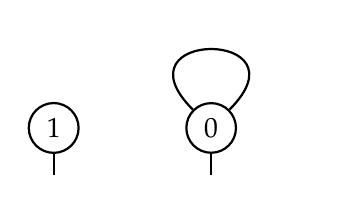
\begin{tikzpicture}[scale=1, transform shape, every loop/.style={}]
    \node[circle,draw=black,thick] (B) at (-1,0) {$1$};
    \draw[-,thick] (B) -- (-1,-0.6);
    \node[circle,draw=black,thick] (A) at (1,0) {$0$};
    \draw[-,thick] (A) -- (1,-0.6);
    \path[every node/.style={font=\sffamily\small},thick]
        (A)   edge[loop] (A);
    \end{tikzpicture}
    \end{center}
    \caption{$g=1, n=1$ 的稳定图}%
    \label{fig:03graphloop}
    \end{figure}
    第一个图 $\Gamma_1$ 给出贡献
    \begin{align*}
        \Cont_{\Gamma_1} &= T\omega_{1,1}^{\E}(R(z)^{-1}\1) \\
        &= \omega_{1,1}^{\E}(R(z)^{-1}\1) + p_* \omega_{1,1}^{\E}(R(z)^{-1}\1, T_R(z)).
    \end{align*}
    利用公式 $B_2 = \frac{1}{6}$ 以及 $\dim \Mbar_{1,1} = 1$ 的事实，上式变为
    \[ 1 - \frac{1}{12}\psi_1 + \frac{1}{12} \kappa_1. \]
    第二个图没有尾部贡献，因为 $\dim \Mbar_{0,3} = 0$。边贡献的常数项是 $\frac{1}{12}$，因此考虑自同构并前推到 $\Mbar_{1,1}$，我们得到
    \[ \Cont_{\Gamma_2} = \frac{1}{12} \Delta, \]
    其中 $\Delta$ 表示边界除子（带有正确的叠结构）。由于此时 $\psi_1 = \kappa_1$，我们得到
    \[ 1+\lambda_1 = 1 + \frac{1}{12}(\kappa_1 - \psi_1 + \Delta) = 1 + \frac{1}{12} \Delta. \]
\end{exm}




\subsection{算符形式与几何量子化}%
\label{sub:Operator formalism and geometric quantization}

我们回到 Givental 的辛形式。它对某些计算更为方便，但事实上它与我们之前的理论相同，至少在我们想要计算生成函数时是如此。回顾我们在 $V$ 上有弗罗贝尼乌斯流形结构，并考虑带辛形式
\[ (\mbf{f}(z), \mbf{g}(z)) \coloneqq \on{Res}_{z=0} \eta(\mbf{f}(-z), \mbf{g}(z)). \]
的向量空间 $\mc{V}\coloneqq V\ls{z^{-1}}$。若考虑由 $\mc{V}_+ = V[z]$ 与 $\mc{V}_- = z^{-1}V\ps{z^{-1}}$ 给出的极化，则令 $\bq$ 如前所述（含膨胀子平移），并取 $\bp$ 为 $\mc{V}_-$ 上的坐标，使得 $(\bq, \bp)$ 构成 $\mc{V}$ 的一组 Darboux 坐标。

\begin{defn}
    我们把任意形如
    \[ \mc{D} = \exp\ab(\sum_{g=0}^{\infty} \hbar^{g-1} \mc{F}_g) \]
    的形式函数称为 \textit{Fock 空间的渐近元}。
\end{defn}

给定这样一个 Fock 空间的渐近元，我们用如下公式对 $\mc{V}$ 上的（无穷小）辛变换进行量子化：
\[ \wh{p_a p_b} \coloneqq \hbar \partial_{q_a} \partial_{q_b}, \qquad \wh{p_a q_b} \coloneqq q_b \partial_{q_a}, \qquad \wh{q_a q_b} = \frac{q_a q_b}{\hbar}. \]
特别地，这将使我们能够理解形如 $\hat{R} \mc{D}$ 的表达式。然而我们需要小心，因为我们的公式中同时涉及基本解 $S_{\tau}$ 与 $R$-矩阵，而 $S_{\tau}$ 是 $z^{-1}$ 的幂级数。\footnote{这是由于我们按 $\frac{1}{z-\psi} = \sum_{n=0}^{\infty} \psi^n z^{-n-1}$ 展开。}

\begin{thm}[Givental {\cite{Givental2001quantization}}]
    形如 $S(z^{-1}) = \mr{Id} + S_1 z^{-1} + \cdots$ 的算符按如下公式作用于 Fock 空间的（渐近）元：
    \[ \hat{S}^{-1} \mc{D}(\bq) = e^{\frac{1}{2\hbar}W(\bq,\bq)} \mc{D}([S \bq]_+), \]
    其中 $W = \sum \eta(W_{mn}q_m, q_n)$ 由如下公式定义：
    \[ \frac{S(w^{-1})^* S(z^{-1}) - \mr{Id}}{w^{-1}+z^{-1}} = \sum \frac{W_{mn}}{w^m z^n}. \]
    形如 $R(z) = \mr{Id} + R_1 z + \cdots$ 的算符按如下公式作用：
    \[ \hat{R}\mc{D}(\bq) = e^{\frac{\hbar}{2} V(\partial_{\bq}, \partial_{\bq})} \mc{D}(R^{-1} \bq), \]
    其中 $V = \sum \eta(p_m, V_{mn} p_n)$ 由如下公式定义：
    \[ \frac{R(w)^* R(z) - \mr{Id}}{w+z} = \sum V_{mn} w^m z^n. \]
\end{thm}

对半单 CohFT，存在一族 \textit{典范坐标} $u_{\alpha}$，使得 $1$-形式 $\d{u}$ 是代数同态 $T_v V \to \C$。于是在半单点附近，量子联络有一个形如
\[ \Psi \cdot  R \cdot e^{\frac{U}{z}}, \]
的渐近解，其中 $\Psi$ 从平坦坐标切换到典范坐标，$U = \on{diag}(u_{\alpha})$ 是典范坐标的矩阵。最后，定义
\[ C = \frac{1}{2} \int^u \sum R_1^{\alpha\alpha} \d{u_{\alpha}}. \]
Teleman 重构定理的一个推论是如下公式
\[ \mc{D}^X = e^{C(u)} \hat{S}^{-1}_{\tau} \hat{\Psi} \hat{R} \wh{e^{\frac{U}{z}}} \prod_{i=1}^{\dim V} \mc{D}^{\mr{pt}} \]
它对任意量子上同调半单的光滑射影簇的格罗莫夫–威滕理论成立。

\begin{exm}
    作为最后一个例子，我们将应用 Teleman 定理来计算任意半单 CohFT 的 $F_1$。设 $e_{\mu}$ 表示量子积的一组幂等基。我们将计算
    \[ \int_{\Mbar_{1,1}} \Omega_{1,1}(e_{\beta}). \]
    利用重构定理，我们得到
    \begin{align*}
        \int_{\Mbar_{1,1}}\Omega_{1,1}(e_{\beta}) ={}& \int_{\Mbar_{1,1}} T_R \omega_{1,1}(R(\bar{\psi})^{-1} e_{\beta}) + \frac{1}{2} T_R \omega_{0,3}(R(\bar{\psi})^{-1} e_{\beta}, V(\bar{\psi}_2, \bar{\psi}_3)) \\
        ={}& \int_{\Mbar_{1,1}}T_R\omega_{1,1}(e_{\beta}) - \int_{\Mbar_{1,1}} T_R \omega_{1,1}(R_1 e_{\beta})\bar{\psi} \\ 
        &+ \frac{1}{2}\sum_{\mu}  \omega_{0,3}(e_{\beta}, R_1 e^{\mu}, e_{\mu}) \\
        ={}& \int_{\Mbar_{1,1}} ( \omega_{1,1}(e_{\beta}) + p_* ( \omega_{1,2}(e_{\beta}, R_1 \1) \bar{\psi}_2^2 )) \\
        &- \int_{\Mbar_{1,1}} (\omega_{1,1}(R_1 e_{\beta})\bar{\psi}_1 + p_* ( \omega_{1,2}(R_1 e_{\beta}) \bar{\psi}_2^2 ) \bar{\psi}_1) \\
        &+ \frac{1}{2} \sum_{\mu} \eta(e_{\beta} \star e_{\mu}, R_1 e^{\mu}) \\
        ={}& \frac{1}{24} \sum_{\mu} ( \omega_{0,4}(e_{\mu}, e^{\mu}, e_{\beta}, R_1 \1) -\omega_{0,3}(e_{\mu}, e^{\mu}, R_1 e_{\beta}) )\\
        &+ \frac{1}{2} \eta(e_{\beta}, R_1 e^{\beta}) \\
        ={}& \frac{1}{24} \sum_{\mu}\sum_{\nu} \omega_{0,3}(e_{\mu}, e^{\mu}, e_{\nu})\omega_{0,3}(e^{\nu}, e_{\beta}, R_1 \1) \\
        &-\frac{1}{24} \sum_{\mu} \omega_{0,3}(e_{\mu}, e^{\mu}, R_1 e_{\beta}) + \frac{1}{2} (R_1)_{\beta\beta} \\
        ={}& \frac{1}{24} \ab(\eta(e^{\beta}, R_1 \1) - \sum_{\mu} \eta(e^{\mu}, R_1 e_{\beta})) + \frac{1}{2} (R_1)_{\beta\beta}.
    \end{align*}
    利用恒等式
    \begin{align*}
        \eta(R_1 \1, e^{\beta}) - \sum_{\mu} \eta(R_1 e_{\beta}, e^{\mu}) &= \sum_{\mu} \Delta_{\mu} \int_{\Mbar_{0,4}} \Omega_{0,4}(e_{\mu}, e_{\mu}, e_{\mu}, e_{\beta}) \\
        &= -\frac{1}{2}\sum_{\mu} \Delta_{\mu} \partial_{u_{\beta}} \Delta_{\mu}^{-1} \\
        &= \frac{1}{2} \sum_{\mu} \partial_{u_{\beta}} \log \Delta_{\mu},
    \end{align*}
    其中 $\Delta_{\mu} \coloneqq \eta(e_{\mu}, e_{\mu})^{-1}$，我们得到结果
    \[ \int_{\Mbar_{1,1}} \Omega_{1,1}(e_{\beta}) = \frac{1}{48} \sum_{\mu} \partial_{u_{\beta}} \log \Delta_{\mu} + \frac{1}{2} (R_1)_{\beta\beta}, \]
    它可以写成富有启发性的形式
    \[ \d{F_1^{\Omega}} = \sum_{\mu} \ab( \frac{\d{\log \Delta_{\mu}}}{48} + \frac{1}{2} (R_1)_{\mu\mu} \d{u_{\mu}} ). \]
    这重现了 Givental 早已知道的一个结果。
\end{exm}

\subsection{如何计算 \(R\)-矩阵}%
\label{sub:How to compute the R-matrix}

最后我们说明如何计算 R-矩阵，先从弗罗贝尼乌斯流形共形的情形开始（例如光滑射影簇的格罗莫夫–威滕理论、\(r\)-spin 曲线等）。在本例中，我们遵循~\cite{PPZ2015} 考虑 3-spin 曲线的弗罗贝尼乌斯流形。设 \(V\) 是 2 维的，坐标为 \(x\) 与 \(y\)，其中 \(x\) 对应于单位。度量由
\[ \eta = \begin{pmatrix}
    0 & 1 \\
    1 & 0
\end{pmatrix} \]
给出，而初级亏格零势为 \(F(x,y) = \frac{1}{2} x^2 y + \frac{1}{72} y^4\)。存在一个 \textit{Euler 向量场}
\[ E = x \pdv{}{x} + \frac{2}{3} y \pdv{}{y}, \]
它分别以权重 \(-1\) 与 \(-\frac{2}{3}\) 作用于 \(\partial_x\) 与 \(\partial_y\)。共形维数为 \(\delta = \frac{1}{3}\)，我们定义次数算符
\[ \mu(v) = [E,v] + \ab(1 - \frac{\delta}{2})v. \]
这里，\(\partial_x\) 的次数为 \(-\frac{1}{6}\)，\(\partial_y\) 的次数为 \(\frac{1}{6}\)。

为使问题简化，我们令 \(\phi = \frac{y}{3}\) 并定义
\[ \hat{\partial}_x = \phi^{1/4} \partial_x, \qquad \hat{\partial}_y = \phi^{-1/4} \partial_y, \]
然后在此标架下进行计算。在此设定下，量子乘法由
\[ \hat{\partial}_x \star \hat{\partial}_x = \phi^{1/4} \hat{\partial}_x, \qquad \hat{\partial}_x \star \hat{\partial}_y = \phi^{1/4} \hat{\partial}_y, \qquad \hat{\partial}_y \star \hat{\partial}_y = \phi^{1/4} \hat{\partial}_x. \]
给出。我们还需要的最后一件事是：用 \(E\) 进行量子乘法由
\[ E \star - = \begin{pmatrix}
    x & 2 \phi^{3/2} \\
    2 \phi^{3/2} & x 
\end{pmatrix}. \]
给出。我们现在利用递推方程
\[ [R_{k+1}, E \star -] = (k + \mu) R_k. \]
来计算 R-矩阵 \(R = 1 + R_1 z + \cdots\)。令 \(R_k = \begin{psmallmatrix}
    a_k & b_k \\
    c_k & d_k
\end{psmallmatrix}\)，我们得到方程
\[ \ab[
    \begin{pmatrix}
        a_{k+1} & b_{k+1} \\
        c_{k+1} & d_{k+1}
    \end{pmatrix}, \begin{pmatrix}
        x & 2 \phi^{3/2} \\
        2 \phi^{3/2} & x 
    \end{pmatrix}
] = \frac{1}{6} \pdiagmat[empty={}]{6k-1, 6k+1} \begin{pmatrix}
    a_k & b_k \\
    c_k & d_k 
\end{pmatrix}. \]

其唯一解实际上是
\begin{align*}
    a_k &= \frac{1}{1728^k \phi^{3k/2}} \frac{1+6k}{1-6k} \frac{(6k)!}{(3k)!(2k)!} \delta_{k, \text{even}},  \\
    b_k &= \frac{1}{1728^k \phi^{3k/2}} \frac{1+6k}{1-6k}\frac{(6k)!}{(3k)!(2k)!} \delta_{k, \text{odd}},  \\
    c_k &= \frac{1}{1728^k \phi^{3k/2}}\frac{(6k)!}{(3k)!(2k)!} \delta_{k, \text{odd}}, \\
    d_k &= \frac{1}{1728^k \phi^{3k/2}} \frac{(6k)!}{(3k)!(2k)!} \delta_{k, \text{even}}. 
\end{align*}
若你熟悉曲线模空间上的重言关系，就会看出级数 \(a_k + b_k\) 与 \(c_k + d_k\) 出现在 Faber-Zagier 关系与 Pixton 关系的表述中。

当弗罗贝尼乌斯流形不共形时（例如在等变格罗莫夫–威滕理论中），我们需要用振荡积分或其他方法来确定 R-矩阵中的初值。这里我们给出一个计算例子，它归于 Givental~\cite{Givental2001semisimple}。在此设定中 \(X = \P^n\)，但该论证对任意 Fano 环面簇也成立。回顾 \(\P^n\) 的等变镜像是超势
\[ W = x_1 + \cdots + x_{n+1} + \sum_{i=1}^{n+1} \lambda_i \log x_i \]
（这里为方便起见我们改变了等变参数的符号）。因此，振荡积分形如
\[ I = \int_{\Gamma \subset E_q = (x_1 \cdots x_{n+1}=q)} e^{W/z} \prod_{i=1}^{n+1} \frac{\d{x_i}}{x_i}. \]
它被算符
\[ \prod_{i=1}^{n+1}\ab(zq \odv{}{q} -\lambda_i) - q, \]
零化，而这正是射影空间的 I-函数所满足的 Picard-Fuchs 方程。

为在临界点附近展开该积分，我们首先需要计算临界点。这里使用坐标 \(t = \log q\) 与 \(T_i = \log x_i\)，得到方程
\[ x_i = L - \lambda_i, \]
其中 \(L\) 是 Lagrange 乘子。它们满足方程
\[ \prod_{i=1}^{n+1} (L - \lambda_i) = q, \]
因此对一般的 \(\lambda\)，在 \(q = 0\) 附近，Lagrange 乘子的可能取值 \(L_i\) 由它们从哪个 \(\lambda_i\) 开始来区分。注意函数 \(W\)、Lagrange 乘子的取值以及临界点都连续依赖于 \(\lambda\)，故当 \(q \neq 0\) 时它们在 \(\lambda = 0\) 处均存在非等变极限。

当 \(q = 0\) 时，矩阵 \(\Psi\) 从平坦基 \(\ab{H^i}\) 过渡到基
\[ L_i(H) = \prod_{j \neq i} \frac{H - \lambda_j}{(\lambda_i - \lambda_j)^{1/2}}, \]
它们是典范坐标的首项（只需通过等变局部化计算环面作用的不动点，我们就会得到这一 Lagrange 插值）。因此，我们需要在 \(q = 0\) 极限下计算 \(L_j \ab(z q \odv{}{q}) I\)。直接计算表明，将 \(L_i \ab(z q \odv{}{q})\) 作用于积分会给振荡积分的被积函数引入一个正比于 \(\frac{q}{x_i}\) 的额外因子。由于我们可以置换指标，我们只计算 \(i = n+1\) 的情形。另一直接计算表明，除非 \( j = n+1\)，否则积分在 \(q = 0\) 处为零，因此实际上我们看到 \(R\) 在经典极限下是对角的。当 \(j = n+1\) 时，我们有
\[ \frac{q}{x_{n+1}} = x_1 \cdots x_n, \]
而积分变为
\[ \int_{\Gamma} e^{\ab( \sum_{i=1}^n x_i + (\lambda_i - \lambda_{n+1})\log x_i ) / z} \d{x_1} \cdots \d{x_n} = \prod_{i=1}^n \int_{\R} e^{x_i/z} x_i^{(\lambda_i - \lambda_{n+1})/z} \d{x_i}, \]
这只是一些 gamma 函数的乘积。

\begin{lem}
    我们有渐近展开
    \[ \log \Gamma(1+s) \sim s \log \ab(\frac{s}{e}) + \frac{1}{2} \log(2\pi s) + \sum_{k=1}^{\infty} \frac{B_{2k}}{2k} \frac{s^{1-2k}}{2k-1}. \]
\end{lem}
由此我们看到，在 \(q = 0\) 处，R-矩阵的对角矩阵元由
\[ \log R = \sum_{k=1}^{\infty} \frac{B_{2k}}{2k} \frac{z^{2k-1}}{2k-1} \sum_{i =1}^n (\lambda_i - \lambda_{n+1})^{1-2k}. \]
给出。由 Givental 的一个结果，这表明该 R-矩阵重现了 \(\P^n\) 的等变 GW 理论；作为推论，由于非等变极限存在，我们得到 \(\P^n\) 的 Virasoro 约束。


\section{半小映射的分解定理（文学清）}%
\label{sec:Decomposition theorem for semi-small maps (Xueqing Wen)}

\begin{quest}
    设 \(X\) 为（流形、簇、解析空间等）。我们如何计算 \(H^*(X, \C)\)？
\end{quest}

遗憾的是，这个问题过于困难，因此我们转而考虑下面的新问题。

\begin{quest}
    我们如何用更小的空间来确定 \(H^*(X, \C)\)？
\end{quest}

\begin{thm}[K\"unneth 公式]
    我们有 \(H^*(X \times Y, \C) = H^*(X, \C) \otimes H^*(Y, \C)\)。
\end{thm}

遗憾的是，大多数空间并不是乘积，于是我们考虑下面的问题。

\begin{quest}
    设 \(f \colon X \to Y\) 为态射。我们能否用 \(Y\) 的上同调与 \(f\) 的纤维的上同调来确定 \(X\) 的上同调？
\end{quest}

这个问题依然非常困难，但至少可以着手研究。我们先考虑 \(f\) 是紧流形之间的纤维丛的情形。答案当然是 Leray 谱序列或 Serre 谱序列，但在此之前，我们需要一些预备知识。

\begin{defn}
    \(Y\) 上的 \(\ul{\C}_Y\)-局部系统是指 \(Y\) 上向量空间的局部常值层 \(\mc{L}\)。
\end{defn}

例如，若 \(Y\) 连通，则局部系统对应于 \(\pi_1(Y)\) 的表示。此外请注意，若 \(Y\) 是代数簇，我们需要改用它的解析化空间。

\begin{exm}
    设 \(f\) 是如上所述的以 \(F\) 为纤维的纤维丛。则 \(R^i f_* \ul{\C}_X\) 是 \(Y\) 上以 \(H^i(F, \C)\) 为纤维的局部系统。
\end{exm}

\begin{prop}
    我们有
    \[ H^*(X, \C) = H^*(X, \ul{\C}_X) = H^*(\mr{pt}, R a_{X*} \ul{\C}_X). \]
\end{prop}

\begin{thm}[Leray/Serre 谱序列]
    我们有谱序列
    \[ E_2^{p,q} = H^p(Y, R^q f_* \ul{\C}_X) \Rightarrow H^{p+q}(X, \C). \]
\end{thm}

现在考虑 \(f \colon X \to Y\) 为光滑射影簇之间的光滑射影态射的情形。

\begin{thm}[Deligne {\cite{Deligne1968}}]
    我们有非典范同构
    \[ R f_* \ul{\C}_X = \bigoplus_{q \geq 0} R^q f_* \ul{\C}[-q]. \]
    在上同调层面，我们有
    \[ H^*(X, \C) = \bigoplus_{q \geq 0} H^{*-q}(Y, R^q f_* \ul{\C}). \]
\end{thm}

这是射影簇的硬莱夫谢茨定理的一个推论，同时也说明 Serre 谱序列在 \(E_2\) 页退化。在拓扑中，Hopf 纤维丛则不满足这一结论。

现在考虑 \(f \colon X \to Y\) 为代数簇之间的真（proper）态射的情形。此时我们有 \textit{Whitney 分层}\footnote{我们明确拒绝给出定义。} \(Y = \bigsqcup_{\lambda} Y_{\lambda}\)，使得 \(f^{-1}(Y_{\lambda}) \to Y_{\lambda}\) 是（可能奇异的）簇之间的 \(C^{\infty}\) 纤维化。

\begin{defn}
    若存在 Whitney 分层 \(Y = \bigsqcup Y_{\lambda}\)，使得对所有 \(\lambda\)，\(\mc{F}|_{Y_{\lambda}}\) 都是局部系统，则称 \(Y\) 上的 \(\ul{\C}_Y\)-模 \(\mc{F}\) 为 \textit{可构造层}。
\end{defn}

由此我们可以考虑 \(Y\) 上可构造层的导出范畴 \(\mc{D}_c^b(Y)\)。这一对应具有六函子形式，其中的函子为 \(f_*, f^*, f_!, f^!, \otimes, \mc{H}\mr{om}\)，并满足 Verdier 对偶，对偶函子为
\[ D_Y \colon \mc{D}_c^b(Y) \to \mc{D}_c^b(Y). \]

\begin{defn}
    复形 \(\mc{F}^{\bullet} \in \mc{D}_c^b(Y)\) 称为 \textit{反常层}，若它满足以下条件：
    \begin{enumerate}
        \item （支撑条件）对所有 \(i\)，我们有 \(\dim \on{supp} \mc{H}^{-i}(\mc{F}^{\bullet}) \leq i\)；
        \item （余支撑条件）对所有 \(i\)，我们有 \(\dim \on{supp} \mc{H}^{-i}(D_Y \mc{F}^{\bullet}) \leq i\)。
    \end{enumerate}
\end{defn}

\begin{rmks}\leavevmode
    \begin{enumerate}
        \item 反常层并非层，而是集中在次数 \([-\dim Y, 0]\) 的复形。
        \item 它们有两个来源：一是相交同调，二是 Riemann-Hilbert 对应。
    \end{enumerate}
\end{rmks}

我们需要用到以下事实：\(Y\) 上反常层的范畴 \(\ms{Perv}(Y)\) 是一个阿贝尔范畴，而且是 \(\mc{D}_c^b(Y)\) 上某个 \(t\)-结构的心。特别地，对任意 \(\mc{G} \in \mc{D}_c^b (Y)\)，我们可以考虑反常上同调 \(^p\mc{H}^i(\mc{G}) \in \ms{Perv}(Y)\)。

\begin{thm}[Beilinson-Bernstein-Deligne-Gabber {\cite{BBD1982}}]
    设 \(f \colon X \to Y\) 为代数簇之间的真态射。假设 \(X\) 光滑且连通。\footnote{这一条件并非必要，但若去掉光滑性假设，我们就需要考虑相交复形。} 则
    \[ R f_* \ul{\C}_X [\dim X] = \bigoplus_{i} {^p\mc{H}^i}(R f_* \ul{\C}_X)[-i]. \]
    此外，每个 \(^p\mc{H}^i (R f_* \ul{\C}_X)\) 都是半单的（即每个子对象都是直和项）。
\end{thm}

\begin{defn}
    设 \(f \colon X \to Y\) 为真满态射，且 \(X\) 光滑、不可约。设 \(Y = \bigsqcup Y_{\lambda}\) 是一个分层，使得 \(f^{-1}(Y_{\lambda}) \to Y_{\lambda}\) 是 \(C^{\infty}\)-纤维化。若对所有 \(y_{\lambda} \in Y_{\lambda}\) 都有 \(\on{codim}_Y Y_{\lambda} \geq 2 \dim f^{-1} (y_{\lambda})\)，则称 \(f\) 是 \textit{半小}的。若等号成立，则称 \(Y_{\lambda}\) 是 \textit{相关的}（relevant）。若唯一的相关层是稠密的那一个，则称 \(f\) 是 \textit{小}的。
\end{defn}

\begin{thm}[{\cite{DeCataldoMigliorini2002}}]
    若 \(f \colon X \to Y\) 是半小的，则 \(R f_* \ul{\C}_X [\dim X]\) 是 \(Y\) 上的反常层。
\end{thm}

\begin{proof}
    对 \(y_{\lambda} \in Y_{\lambda} \subseteq Y\)，我们有
    \[ R f_* \ul{\C}_X |_{y_{\lambda}} = \bigoplus H^i (f^{-1}(y_{\lambda}), \C). \]
    注意到当 \(i > 2 \dim f^{-1}(y_{\lambda}) \leq \on{codim}_Y (Y_{\lambda})\) 时上式为零。当 \(Y_{\lambda}\) 取遍所有层时，我们得到支撑条件。由于 \(f\) 是真态射，有 \(R f_* = f_!\)，再利用 \(D_Y R f_* = f_! D_X\)，我们得到余支撑条件。
\end{proof}

\begin{exms}
    下面我们给出半小映射的一些例子。
    \begin{enumerate}
        \item 曲面之间任意泛有限的真映射都是半小的。
        \item 设 \(Y = \ab\{xy = t^{\ell+1}\} \subseteq \C^3\)。则有奇点的 crepant 消解（crepant resolution）\(f \colon \tilde{Y} \to Y\)，且奇异点上的纤维是一条 \(\P^1\) 的链，因此它是半小的（另见上一个例子）。
    \end{enumerate}
\end{exms}

\begin{thm}[Kaledin {\cite{Kaledin2006}}]
    从非奇异全纯辛簇出发的射影双有理映射是半小的。
\end{thm}

\begin{exm}
    例如，Springer 消解与 Grothendieck-Springer 消解都是半小的。此外，曲面上点的希尔伯特概形的 Hilbert-Chow 态射也是半小的。
\end{exm}

设 \(f \colon X \to Y\) 半小，并考虑分层 \(Y = \bigsqcup Y_{\lambda}\)。若 \(Y_{\lambda}\) 相关，考虑
\[ \mc{L}_{\lambda} = R^{d_{\lambda}} f_* \ul{\C}_{f^{-1}(Y_{\lambda})}, \]
其中 \(d_{\lambda} = 2 \dim f^{-1} (y_{\lambda})\)。则 \(\mc{L}_{\lambda}\) 是半单的。这里请注意 \(\mc{L}_{|\lambda} = H^{d_{\lambda}}(f^{-1}(y_{\lambda}), \C)\)。现在设 \(\mr{IC}(\mc{L}_{\lambda})\) 为 \(\mc{L}_{\lambda}[\dim Y_{\lambda}]\) 在 \(\ol{Y}_{\lambda}\) 上的中间扩张，这是一个反常层。

\begin{thm}[{\cite{DeCataldoMigliorini2002}}]
    设 \(f \colon X \to Y = \bigsqcup Y_{\lambda}\) 半小。则有典范分解
    \[ R f_* \ul{\C}_X[\dim X] = \bigoplus_{Y_{\lambda}\text{ relevant}} \mr{IC}(\mc{L}_{\lambda}). \]
\end{thm}

\begin{exm}
    设 \(G\) 是以 \(\g\) 为李代数的约化群，并取 Borel 子群 \(B\)。则
    \[ G \times_B \b = \tilde{\g} \xrightarrow{\pi} \g \]
    是小的。因此我们有
    \[ R \pi_* \ul{\C}_{\tilde{\g}} [\dim \g] = \mr{IC}(\mc{L}). \]
    回顾 \(\tilde{\g}^{\on{rs}} \to \g^{\on{rs}}\) 是一个 \(W\)-扭。于是对 \(a \in \g^{\on{rs}}\)，有 \(\mc{L}_{|a} \cong \C[W]\)，因而 \(\mc{L} = R^0 \pi_* \ul{\C}_{\tilde{\g}^{\on{rs}}}\)。这意味着 \(W\) 作用在 \(\mc{L}\) 上，且该作用可以延拓到 \(\mr{IC}(\mc{L})\) 上，也可以延拓到 \(R \pi_* \C_{\tilde{\g}}\) 上，特别地它作用在任意 \(a \in \g\) 处的纤维 \(R \pi_* \C_{\tilde{\g}}|_a\) 上。
\end{exm}

\begin{exm}
    考虑 Springer 消解 \(\mu \colon T^*(\on{GL}_3/B) \to \mc{N} = \mathbb{O}_{(1^3)} \sqcup \mathbb{O}_{(2,1)} \sqcup \mathbb{O}_{(3)}\)。该映射是半小的，但遗憾的是所有幂零轨道都是相关的。注意到 \((2,1)\) 轨道上的纤维是两条 \(\P^1\) 沿一个结点粘合而成的并，\((3)\) 轨道上的纤维是一个点，而 \((1^3)\) 轨道上的纤维是 \(\on{GL}_3/B\)。

    我们看到 \(\mc{L}_{(3)}\) 必然是平凡的，因为 \(\mu\) 在该轨道上方是同构。于是 \(\mc{L}_{(2,1)} = R^2 \mu_* \ul{\C}\) 是 \(\mathbb{O}_{(2,1)}\) 上的秩 \(2\) 局部系统。最后，\(\mc{L}_{(1^3)} = R^6 \mu_* \ul{\C}\) 是 \(\mathbb{O}_{(1^3)} = \mr{pt}\) 上的秩 \(1\) 局部系统。因此我们有
    \[ R \mu_* \ul{\C}_{T^*\on{GL}_3/B}[6] = \mr{IC}(\mc{L}_{(3)}) \oplus \mr{IC}(\mc{L}_{(2,1)}) \oplus \mr{IC}(\mc{L}_{(1^3)}). \]
    限制到 \(b \in \mathbb{O}_{(3)}\) 上，我们得到 \(\mc{L}_{(3)} = H^0(\mr{pt})\)。限制到 \(a \in \mathbb{O}_{(2,1)}\) 上，我们得到
    \[ H^0(X, \C) \oplus H^2(X, \C) = \mr{IC}(\mc{L}_{(3)})|_{(a)} \oplus \mr{IC}(\mc{L}_{(2,1)})|_{(a)}. \]
    限制到 \(0 = \mathbb{O}_{(1^3)}\) 上，我们得到
    \begin{align*}
        H^*(\on{GL}_3/B, \C) = \C[W] &= \mr{IC}(\mc{L}_{(3)})|_0 \oplus \mr{IC}(\mc{L}_{(2,1)})|_0 \oplus \mc{L}_{(1^3)}|_0 \\
        &= H^0(\on{GL}_3/B, \C) \oplus \ab(\text{a summand of dimension } 4) \oplus H^6(\on{GL}_3/B, \C).
    \end{align*}
    作为 \(W = S_3\) 的表示，它们分别对应平凡表示、两份标准表示和符号表示。关于 Springer 理论意义上的构造以及这些分解，见~\cite{BorhoMacPherson1983}。
\end{exm}


\section{量子 K 理论（阎霄汉与周祐正）}%
\label{sec:Quantum K-theory (Xiaohan Yan and You-Cheng Chou)}

\subsection{概述}%
\label{sub:Overview}

格罗莫夫–威滕不变量是某种"计数"光滑射影簇 \(X\) 中曲线的方式。GW 理论给出形如
\[ \ab<\alpha_1, \ldots, \alpha_n>_{g, n, \beta} \in \Q \]
的数，其中 \(\alpha_i \in H^*(X)\) 取各种类，\(g\) 为亏格，\(n\) 为标记点个数，\(\beta \in H_2(X, \Z)\) 为曲线类。这已被用于研究镜像对称，并且在镜像对称之外还给出了双有理不变量。我们现在的目标是把整套理论提升到 K 理论。量子 K 理论给出数
\[ \ab<V_1, \ldots, V_n>_{g, n, \beta} \in \Z \]
其中 \(V_1, \ldots, V_n \in K(X)\)。它们满足各种差分方程\footnote{与上同调中的微分方程作对比。}，并在三维镜像对称与表示论中有各种应用。

\subsection{K 理论}%
\label{sub:K-theory}

\begin{defn}
    设 \(X\) 为光滑射影簇。则 \(X\) 的 \textit{K 理论} \(K(X)\) 是 \(X\) 上向量丛的 Grothendieck 群，其关系为：若
    \[ 0 \to V_1 \to V_2 \to V_3 \to 0 \]
    是短正合列，则 \(V_2 = V_1 + V_3\)。
\end{defn}

\begin{rmk}\leavevmode
    \begin{enumerate}
        \item \(K(X)\) 关于直和与张量积运算构成一个环；
        \item 陈特征标给出同构 \(K(X) \to A^*(X)\)，至少在 \(\Q\) 上成立。
    \end{enumerate}
\end{rmk}

\begin{exm}
    取 \(X = \P^n\)，并令 \(P = \mc{O}(-1)\)。则有
    \[ K(X) = \C[P^{\pm 1}]/(P-1)^{n+1} \xrightarrow{\on{ch}} A^*(X) = \C[H]/H^{n+1}. \]
\end{exm}

对于不假设光滑的 Deligne-Mumford 叠，有两个版本
\[ K_0(X) \supset K^0(X), \]
其中 \(K_0\) 表示凝聚层，\(K^0\) 表示完美复形。二者在光滑射影簇上一致，故从现在起 \(K(X)\) 表示 \(K_0(X)\)。有张量积
\[ K^0(X) \otimes K_0(X) \to K_0(X) \]
以及沿真态射的推前
\[ f_* \colon K(X) \to K(Y) \qquad V \mapsto \sum (-1)^i R^i f_* V \]
若 \(f\) 是完美态射（例如平坦、正则嵌入等），则有拉回
\[ f^* \colon K(Y) \to K(X) \qquad W \mapsto \sum (-1)^i \on{Tor}_i^{f^{-1} \mc{O}_Y} (\mc{O}_X, f^{-1} W). \]

\subsection{曲线模空间}%
\label{sub:Moduli of curves}

回忆到 \(X\) 的稳定映射的模空间
\[ \bar{M}_{g,n}(X, \beta) = \ab\{ f \colon (\Sigma, p_1, \ldots, p_n) \to X \mid g(\Sigma) = g, f_*[\Sigma] = \beta, \abs{\Aut f} < \infty \} \]
它带有求值映射
\[ \ev_i \colon \bar{M}_{g,n}(X, \beta) \to X \qquad (f, \Sigma, \ul{p}) \mapsto f(p_i). \]
还有泛余切线 \(L_i = \sigma_i^* \omega_{ \mc{C}/\bar{M} }\)。

该模空间是真 DM叠，带有一个完美障碍理论，从而给出虚结构层 \(\mc{O}^{\vir}_{g,n,\beta}\)。它来自\textit{虚切丛}的结构，其中
\[ \mathbb{T}_{(f, \Sigma, \ul{p})} \bar{M}_{g,n}(X, \beta) = \chi(\Sigma, f^* T_X) - \chi(\Sigma, T_{\Sigma}(-p_1 - \cdots - p_n)). \]
粗略地说，若 \(\bar{M}\) 是簇 \(Y\) 上向量丛 \(E\) 的某个截面的零轨迹，则 \(\mc{O}^{\vir} = \mc{O}_Y \otimes \mr{Eu}(E)\)，其中 K 理论欧拉类为 \(\mr{Eu}(E) = \sum (-1)^i \Lambda^i E^{\vee}\)。

\subsection{KGW 不变量}%
\label{sub:KGW invariants}

量子 K 理论参见~\cite{Lee2004}；置换等变理论参见~\cite{Givental2017K1,GiventalK7}。To\"en~\cite{Toen1999} 证明了下文所用的 Deligne--Mumford 叠的 Riemann--Roch 公式。

\begin{defn}
    K 理论 GW 不变量定义为
    \[ \ab<V_1, \ldots, V_n>_{g,n,\beta} \coloneqq \chi\ab(\bar{M}_{g,n}(X, \beta); \mc{O}^{\vir} \otimes \bigotimes_{i=1}^n \ev_i^* V_i). \]
\end{defn}

若 \(V_1, \ldots, V_n\) 是真正的向量丛，则该不变量是整数；但一般我们考虑系数在特征零域上的 \(K_0\)。我们也可以定义引力后代
\[ \ab<V_1 L_1^{k_1}, \ldots, V_n L_n^{k_n}>_{g,n,\beta} \coloneqq \chi\ab(\bar{M}_{g,n}(X, \beta); \mc{O}^{\vir} \otimes \bigotimes_{i=1}^n ( \ev_i^* V_i )L_i^{k_i} ). \]
利用 \(S_n\) 通过置换标记点在 \(\bar{M}_{g,n}(X, \beta)\) 上的作用，则对象 \(\bigotimes_{i=1}^n \ev_i^* V\) 与 \(\bigotimes_{i=1}^n L_i^k\) 都是 \(S_n\)-等变的。

\begin{defn}
    我们定义\textit{置换不变的 K 理论 GW 不变量}为
    \begin{align*}
        \ab<V L_1^k, \ldots, V L_n^k>_{g,n,\beta}^{S_n} &\coloneqq \chi\ab([ \bar{M}_{g,n}(X, \beta)/S_n ]; \mc{O}^{\vir} \otimes \bigotimes_{i=1}^n ( \ev_i^* V ) L_i^k) \\
        &= \dim \chi_{S_n} \ab(\bar{M}_{g,n}(X, \beta); \mc{O}^{\vir} \otimes \bigotimes_{i=1}^n ( \ev_i^* V ) L_i^k )^{S_n}.
    \end{align*}
\end{defn}

给定 \(t(q) = \sum_{n \in \Z} t_n q^n \in K(X)[q,q^{-1}]\)，我们可以定义
\[ \ab< t(L_1), \ldots, t(L_n)>^{S_n}_{g,n,\beta} \coloneqq \chi ([\bar{M}_{g,n}(X,\beta)/S_n], \cdots). \]
更一般地，若 \(H = S_{a_1} \times \cdots \times S_{a_m} \subset S_n\)，我们可以定义
\[ \ab<t_1(L_1), \ldots, t_1(L_{a_1}), t_2(L_{a_1+1}), \ldots, t_2(L_{a_1+a_2}), \ldots>_{g,n,\beta}^H. \]

\begin{rmk}
    我们想讨论与普通 GW 不变量的一些联系。回忆 Hirzebruch-Riemann-Roch 定理：
    \[ \chi(M; V) = \int_M \on{ch}(V) \on{td}(T_M). \]
    当 \(M\) 是光滑 DM叠时，T\"oen 证明了公式
    \[ \chi(M; V) = \int_{IM} \wt{\on{ch}}(V) \wt{\on{td}}(T_M), \]
    其中 \(IM = M \times_{\Delta, M \times M, \Delta} M\) 是 \(M\) 的惯性叠，波浪号表示取 orbifold 陈特征标与托德类。
\end{rmk}

\begin{exm}
    若 \(M = B\mu_r\)，则 \(IM = \bigsqcup_{g \in \mu_r} B \mu_r\)。若 \(M = \P(1, r)\) 是加权 \(\P^1\)，则 \(IM = M \sqcup \bigsqcup_{g \neq 1 \in \mu_r} B\mu_r\)。
\end{exm}

\begin{exm}
    取 \(M = BG\)，其中 \(G\) 为有限交换群，\(V\) 为 \(BG\) 上的向量丛，这等同于 \(G\) 的一个表示。则 \(\chi(M, V) = \dim V^G\)。另一方面，我们有
    \[ \int_{IM} \wt{\on{ch}}(V) \cdot \wt{\on{td}}(T_M) = \int_{IM} \on{tr}_g V = \sum_{g \in G} \frac{1}{\abs{G}} \on{tr}_g V = \dim V^G, \]
    故我们在此情形下验证了 Riemann-Roch。
\end{exm}

\subsection{公理性质}%
\label{sub:Axiomatic properties}

\begin{lem}[{\cite{GiventalK7}}]
    我们有\textit{弦方程}
    \begin{align*}
        \ab< 1, x_1(L), \ldots, x_k(L), t, \ldots, t >_{g, 1+k+n, \beta}^{S_n} = \ab<x_1(L), \ldots, x_k(L), t^{\otimes n}>^{S_n}_{g,k+n,\beta} \\
        + \sum_i \ab< \cdots, \frac{x_i(L) - x_i(1)}{L-1}, \ldots, t^{\otimes n}>^{S_n}_{g,k+n,\beta}. 
    \end{align*}
\end{lem}

\begin{proof}
    证明与 GW 理论中相同，来自沿映射 \(\pi \colon\bar{M}_{g,n+1}(X,\beta) \to \bar{M}_{g,n}(X,\beta)\) 计算 \(\pi^* L_i\)。
\end{proof}

\begin{lem}[{\cite{GiventalK7}}]
    我们有\textit{膨胀子方程}
    \begin{align*}
        \ab<L-1, x_1(L), \ldots, x_k(L), t^{\otimes n}>_{g,1+k+n,\beta}^{S_n} ={}& (k-2)\ab<x_1(L), \ldots, x_k(L), t^{\otimes n}>_{g,k+n,\beta}^{S_n} \\
        &+ \ab<x_1(L), \ldots, x_k(L), t, t^{\otimes n-1}>_{g,k+n,\beta}^{S_{n-1}}.
    \end{align*}
\end{lem}

\begin{proof}
    我们用到
    \[ \pi_* L = k + \on{Ind}_{S_{n-1}}^{S_n}(1) - 1, \]
    其中 \(\pi\) 遗忘第一个标记点，\(L = \omega_{\pi} (p_1 + \cdots + p_n)\)。这由存在留数映射
    \[ H^0(L) \xrightarrow{\on{Res}} \bigoplus_{i=1}^{k+n} \C p_i \xrightarrow{\sum} \C. \]
    得到。中间项是 \(k\) 个平凡表示与一个标准表示的直和。
\end{proof}

\begin{notn}
    固定 \(\tau, t \in K(X)\)。记
    \[ \ab<\!\ab<x_1(L_1), \ldots, x_k(L_k)>\!>_{g,k} \coloneqq \sum_{m,n,\beta} \frac{Q^{\beta}}{m!} \ab<x_1(L_1), \ldots, x_k(L_k), \tau^{\otimes m}, t^{\otimes n}>_{g,k+m+n,\beta}^{S_n}. \]
    取 \(\{\phi_{\alpha}\}\) 为 \(K(X)\) 的一组基，\(\{\phi^{\alpha}\}\) 为对偶基。定义配对
    \[ g_{\alpha\beta} = \chi(X, \phi_{\alpha} \otimes \phi_{\beta}). \]
    这并不是正确的配对，故我们考虑
    \[ G_{\alpha\beta} = g_{\alpha\beta} + \ab<\!\ab<\alpha,\beta>\!>_{0,2}. \]
    再取 \(g^{\alpha\beta} = (g_{\alpha\beta})^{-1}\) 以及 \(G^{\alpha\beta} = (G_{\alpha\beta})^{-1}\)。
\end{notn}

\begin{lem}[{\cite{Givental2000K}}]
    给定 \(A,B,C,D \in K(X)[q,q^{-1}]\)，我们有\textit{WDVV 方程}
    \begin{align*}
        \sum_{\alpha,\beta} \ab<\!\ab< A(L), B(L), \phi_{\alpha}>\! >_{0,3}& G^{\alpha\beta}\ab<\!\ab< C(L), D(L), \phi_{\beta}>\! >_{0,3} \\
        &= \sum_{\alpha,\beta} \ab<\!\ab< A(L), C(L), \phi_{\alpha}>\! >_{0,3} G^{\alpha\beta}\ab<\!\ab< B(L), D(L), \phi_{\beta}>\! >_{0,3}. 
    \end{align*}
\end{lem}

\begin{proof}
    将 \(\bar{M}_{0,4} = \P^1\) 上边界除子的等式拉回。在 K 理论中，当 \(D = \bigcup C_i\) 时，我们需要用容斥原理来联系 \(\mc{O}_D\) 与 \(\mc{O}_{C_i}\)，这解释了 \(G^{\alpha\beta}\) 的出现。
\end{proof}

\subsection{环路空间形式}%
\label{sub:Loop space formalism}

\begin{defn}
    \textit{环路空间} \((\mc{K}, \Omega)\) 由
    \[ \mc{K} = K(X)(q) \ps{Q}\]
    配上辛形式
    \[ \Omega(f, g) = - \on{Res}_{q = 0, \infty} \ab<f(q^{-1}), g(q)>_X \frac{\d{q}}{q}. \]
\end{defn}

\begin{rmk}
    有极化 \(\mc{K} = \mc{K}_+ \oplus \mc{K}_-\)，其中
    \[ \mc{K}_+ = K(X)[q, q^{-1}]\ps{Q} \]
    以及
    \[ \mc{K}_- = \ab\{ \frac{f}{g} \mid f, g \in K(X)\ps{Q}[q], g(0) \neq 0, \deg f < \deg g\}. \]
    例如 \(\frac{1}{1-q} \in \mc{K}_-\)。
\end{rmk}

\begin{defn}
    \textit{大 J-函数} \(J \colon \mc{K}_+ \to \mc{K}\) 由下式给出：
    \[ \mathbf{t} = \mathbf{t}(q) \mapsto 1 - q + \mathbf{t}(q) + \sum_{\beta, \alpha} Q^{\beta} \phi^{\alpha} \ab< \frac{\phi_{\alpha}}{1-qL}, \mathbf{t}(L)^{\otimes n}>_{0, 1+n, \beta}^{S_n}. \]
\end{defn}

\begin{rmk}
    注意到应用 Riemann-Roch，我们有
    \begin{align*}
        \chi\ab([\bar{M}/S_n], \frac{1}{1-qL}) &= \int_{I[\bar{M}/S_n]} \on{ch}\ab(\frac{1}{1-qL}) \on{td}.
    \end{align*}
    每一项都化为 \(\on{ch}\ab(\on{tr}_g \frac{1}{1-qL})\) 的形式，这给出某个单位根 \(\zeta\) 对应的形如 \(\on{ch}\ab(\frac{1}{1-q\zeta L})\) 的表达式。于是我们可以展开
    \[ \frac{1}{1-q\zeta L} = \frac{1}{(1-q \zeta) - q\zeta (L-1)} = \sum_k \frac{(q\zeta)^k}{(1-q\zeta)^{k+1}}(L-1)^k. \]
\end{rmk}

\begin{defn}
    \textit{Givental 锥}定义为 \(\mc{L} \coloneqq \Ima J \subset \mc{K}\)，其中我们在 \(Q\)-进拓扑下考虑 \(1-q\) 附近的芽。
\end{defn}

\begin{exm}
    取 \(X = \P^n\)。则我们看到
    \[ J(0) = (1-q) \sum_{d \geq 0} \frac{Q^d}{\prod_{\ell=1}^d (1-Pq^{\ell})^{n+1}}, \]
    其中 \(P = \mc{O}(-1)\)。同前，我们可以展开
    \[ \frac{1}{1-P q^{\ell}} = \frac{1}{(1-q^{\ell}) - q^{\ell}(P-1)} = \sum_{k=0}^{\infty} \frac{q^{\ell k}}{(1-q^{\ell})^{k+1}}(P-1)^k. \]
\end{exm}

\begin{prop}[{\cite{GiventalK7}}]
    事实上，\(\mc{L}\) 确实是 \(\mc{K}\) 中的一个锥，并且我们有
    \[ \mc{L} = \bigcup_{t \in K(X)\ps{Q}} (1-q) S_{t}^{-1}(q) \mc{K}_+. \]
\end{prop}

我们还可以引入"超大"J-函数
\[ J(\mathbf{t}, \tau) = 1-q + \mathbf{t}(q) + \tau + \sum_{\beta, k, \alpha} \frac{Q^{\beta}}{k!} \phi^{\alpha} \ab< \frac{\phi_{\alpha}}{1-qL}, \mathbf{t}(L)^{\otimes n}, \tau^{\otimes k}>_{0,1+n+k,\beta}^{S_n}. \]
若固定 \(\mathbf{t}(q)\)，则 \(J(\tau)\) 来自 \(\tau\) 上弗罗贝尼乌斯流形的一个\textit{微分方程}的基本解。此外，\(\mc{L}^{\mathbf{t}}=  \Ima J(\tau)\) 实际上是拉格朗日锥。

\begin{exm}
    考虑由 Adams 运算给出的 \(f \colon \C[\Lambda_1^{\pm}, \Lambda_2^{\pm}] \to \C[\Lambda_1^{\pm}, \Lambda_2^{\pm}]\)：
    \[ t \mapsto \on{tr}_{(1\cdots n)} t^{\otimes n} = \Psi^n (t). \]
    因此它把 \(\Lambda_1 \mapsto \Lambda_1^n\) 且 \(\Lambda_2 \mapsto \Lambda_2^n\)。然而，如何对 \(t\) 求导并不清楚，因为我们会需要 \(nv t^{n-1} = \Psi^n(v)\)，所以 J-函数不满足关于 \(\mathbf{t}\) 的量子微分方程。
\end{exm}

\subsection{等变 K 理论与局部化}%
\label{sub:Equivariant K-theory and localization}

不动点递归与射影空间计算参见~\cite{GiventalK2}。

设环面 \(T = (\C^{\times})^r\) 作用在光滑射影簇 \(X\) 上。

\begin{defn}
    \textit{等变 K 理论} \(K_T(X)\) 是 \(X\) 上 \(T\)-等变向量丛的 Grothendieck 群。
\end{defn}

\begin{exm}
    例如我们有
    \[ K_T(\on{pt}) = \on{Rep}(T) = \C[\Lambda_1^{\pm}, \ldots, \Lambda_r^{\pm}], \]
    其中 \(\Lambda_i\) 是权为 \((0, \ldots, 1, \ldots, 0)\) 的 \(1\) 维表示。
\end{exm}

\begin{rmk}
    对任意 \(X\)，\(K_T(X)\) 是一个 \(K_T(\mr{pt})\)-代数。
\end{rmk}

\begin{exm}
    考虑 \(\P^n\) 的全等变 K 理论。则我们有
    \[ K_T(\P^n) = \C[P^{\pm}, \Lambda_0^{\pm}, \ldots, \Lambda_n^{\pm}] \big/ \prod_{i=0}^n (P-\Lambda_i). \]
    取 \(\Lambda_i = 1\)，就回到非等变 K 理论。
\end{exm}

\begin{defn}
    我们可以把等变欧拉示性数定义为推前
    \[ \chi_T = \pi_* \colon K_T(X) \to K_T(\mr{pt}). \]
\end{defn}

\begin{exm}
    例如我们有 \(\chi_T(\mc{O}_{\P^1}(1)) = \Lambda_0^{-1} + \Lambda_1^{-1}\)。类似地，我们有
    \[ \chi_T(\mc{O}(2)) = \Lambda_0^{-2} + \Lambda_0^{-1} \Lambda_1^{-1} + \Lambda_1^{-2}. \]
\end{exm}

\begin{notn}
    注意到 \(\on{Frac}(T) = \on{Frac}(\on{Rep}(T))\)。于是我们令
    \[ K_T^{\loc}(X) \coloneqq \on{Frac}(T) \otimes_{\on{Rep}(T)} K_T(X). \]
\end{notn}

我们将需要下述事实。设 \(F\) 为 \(T\) 在 \(X\) 上的不动点集，考虑 \(\iota \colon F \hookrightarrow X\)。则有 \(\on{Frac}(T)\)-代数的同构
\[ K_T^{\loc}(X) \xrightarrow{\iota^*} K_T^{\loc}(F). \]

\begin{rmk}
    其逆由
    \[ (\iota^*)^{-1} = \bigoplus_{i=1}^r \frac{\iota_{i*}}{\on{Eu}(N_{F_i/X})}, \]
    给出，其中 \(\on{Eu}(V) \coloneqq \sum_{j = 0}^{\on{rk} V} (-1)^j \Lambda^j V^*\) 是 K 理论欧拉类。
\end{rmk}

\begin{exm}
    在 \(\P^n\) 上有 \(n+1\) 个孤立不动点 \(F_i\)，于是我们得到
    \[ \frac{\iota_{i*} \mc{O}_{F_i}}{\on{Eu}(N_{F_i/\P^n})} = \prod_{j \neq i} \frac{P - \Lambda_j}{\Lambda_i - \Lambda_j}. \]
    这些是 \(K_T^{\loc}(\P^n)\) 的幂等元。
\end{exm}

利用等变局部化，我们得到
\[ \chi_T(X; V) = \sum_i \chi\ab(F_i; \frac{\iota_i^* V}{\on{Eu}(N_{F_i/X})}). \]

\begin{rmk}
    在 \(\Lambda = 1\) 的极限下，我们可以恢复非等变欧拉示性数。
\end{rmk}

\begin{exm}
    取 \(X = \P^1\)。计算如下
    \begin{align*}
        \chi_T(\P^1, \mc{O}(1)) &= \chi\ab(F_0, \frac{\mc{O}(1)|_{F_0}}{\on{Eu}(T_{F_0/\P^1})}) + \chi\ab(F_1, \frac{\mc{O}(1)|_{F_1}}{\on{Eu}(T_{F_1/\P^1})}) \\
        &= \frac{\Lambda_0^{-1}}{1 - \frac{\Lambda_0}{\Lambda_1}} + \frac{\Lambda_1^{-1}}{1 - \frac{\Lambda_1}{\Lambda_0}} \\
        &= \Lambda_0^{-1} + \Lambda_1^{-1}. 
    \end{align*}
\end{exm}

从现在起假设 \(X\) 是 GKM 流形。我们现在的目标是利用 \(\bar{M}_{g,n}(X, \beta)\) 上的局部化来研究 \(X\) 的大 J-函数。任何 \(T\)-不动的稳定映射 \(f \colon (\Sigma, \ul{p}) \to X\) 有两类不可约分支：一类完全映到不动点，另一类通过 \(1\) 维轨道的分歧覆盖映出。遗憾的是，我们无法用虚局部化计算大 J-函数，但仍可以研究它。

设 \(f = f(q) \in \mc{K} = K_T^{\loc}(X)(q)\ps{Q}\)。记不动点为 \(F_{\alpha}\)（\(\alpha = 1, \ldots, r\)），包含映射为 \(\iota_{\alpha} \colon F_{\alpha} \hookrightarrow X\)。再记
\[ f_{\alpha}(q) = \iota_{\alpha}^* f(q) \in K_T^{\loc}(\on{pt})(q)\ps{Q}. \]
则 \(f \in \mc{L}\) 当且仅当对所有 \(\alpha\) 下列条件成立：
\begin{enumerate}
    \item 给定 \(\lambda \in T_{F_{\alpha}} X\) 与 \(m \in \N_+\)，\(f_{\alpha}(q)\) 在 \(q = \lambda^{1/m}\) 处至多有单极点，且
        \[ \on{Res}_{q = \lambda^{1/m}} f_{\alpha}(q) \frac{\d{q}}{q} = -\frac{Q^m}{m} \cdot \frac{\on{Eu}(T_{F_{\alpha}/X})}{\on{Eu}(T^{\vir}_{\phi_{\alpha,\alpha',m}}\bar{M}_{0,2}(X, m \cdot \beta(\alpha, \alpha')))} \cdot f_{\alpha'}(\lambda^{1/m}). \]
        这里 \(\lambda \in T_{F_{\alpha}}X\) 意思是 \(\lambda\) 是 \(T_{F_{\alpha}} X\) 的一个 \(1\) 维子表示。此外，\(\beta(\alpha,\alpha')\) 是由权 \(\lambda\) 决定的 \(T\) 的 \(1\) 维轨道的次数，而 \(\phi_{\alpha, \alpha', m}\) 参数化该 \(1\) 维轨道的 \(m:1\) 覆盖。
    \item \(f_{\alpha}(q)\) 的其余极点位于 \(0, \infty\) 与单位根处，在别处正则。此外还有若干次要条件。
\end{enumerate}

\begin{exm}
    取 \(X = \P^n\)。则
    \[ J_T^X(0) = (1-q) \sum_{d \geq 0} \frac{Q^d}{\prod_{i=0}^n \prod_{\ell = 1}^d \ab(1 - \frac{P}{\Lambda_i} q^{\ell})} \in K_T(X)(q) \ps{Q}. \]
    这进而推出
    \[ J_T^X(0) |_{F_j} = (1-q) \sum_{d \geq 0} \frac{Q^d}{\prod_{i=0}^n \prod_{\ell = 1}^d \ab(1 - \frac{\Lambda_j}{\Lambda_i}q^{\ell})}, \]
    故极点位于 \(q = \ab(\frac{\Lambda_i}{\Lambda_j})^{1/\ell}\)。还要注意
    \[ T_{F_j} X = \frac{\Lambda_0}{\Lambda_j} + \cdots + \frac{\Lambda_n}{\Lambda_j} - 1. \]
\end{exm}

\subsection{量子 K/GV 对应}%
\label{sub:Quantum K/GV correspondence}

五次三维簇的对应于~\cite{GaroufalidisScheidegger2022} 中提出猜想，并在~\cite{ChouLeeQuintic} 中证明。下述 Calabi--Yau 三维簇公式属于 Chou--Lee~\cite{ChouLee2025}。

我们这里的目标是在 Calabi-Yau 三维簇上计算 \(J^K(0)\)。下述结果由 Jockers-Mayr 与 Garoufalidis-Scheidegger 猜想。

\begin{thm}[{\cite{ChouLee2025}}]
    我们有
    \begin{align*}
        J^K(0) &\coloneqq (1-q) + \sum_{\beta, \alpha} Q^{\beta} \Phi^{\alpha} \ab<\frac{\Phi_{\alpha}}{1-qL}>_{0,1,\beta}^{X,K} \\
        &= (1-q) + \sum_{\beta} \sum_{r=1}^{\infty} \mr{GV}_{\beta} Q^{r\beta} \ab[\sum_{j=1}^{n_1} \Phi^{1j} a(r, q^r) + \Phi^{01} b(r, q^r)],
    \end{align*}
    其中 \(\ab\{\Phi_{\alpha}\}_{\alpha=1}^N\) 是 \(K^0(X)\) 的一组基，并作如下分解
    \[ \ab\{\Phi_{\alpha}\}_{\alpha=1}^N = \bigsqcup_{i=0}^3 \ab\{\Phi_{ij}\}_{j=1}^{n_i} \]
    使得对固定的 \(i\)，\(\ch(\Phi_{ij})\) 构成 \(H^{2i}(X)\) 的一组基。然后我们选取对偶基 \(\ab\{\Phi^{\alpha}\}_{\alpha} = \ab\{\Phi^{ij}\}_{i,j}\)。此外，我们取多重覆盖公式
    \begin{align*}
        a(r, q^r) &= \frac{r-1}{1-q^r} + \frac{1}{(1-q^r)^2}, \\
        b(r, q^r) &= \frac{r^2-1}{1-q^r} + \frac{3}{(1-q^r)^2} - \frac{2}{(1-q^r)^3}.
    \end{align*}
    最后，GV 表示 Gopakumar-Vafa 不变量，它在亏格零由
    \[ \mr{GW}_{0,\beta} = \sum_{r \mid \beta} \frac{1}{r^3} \mr{GV}_{\beta/r}. \]
    定义。由 M\"obius 反演，我们得到
    \[ \mr{GV}_{\beta} = \sum_{r \mid \beta} \frac{\mu(r)}{r^3} \mr{GW}_{0,\beta/r}. \]
\end{thm}

\begin{cor}[{\cite{ChouLee2025}}]
    我们有
    \[ \ab<1>_{0,1,\beta}^K = \sum_{r \mid \beta} r^2 \mr{GV}_{\beta/r}. \]
    应用 M\"obius 反演，我们得到\footnote{注意到这一结果由 Ionel--Parker~\cite{IonelParker2018} 在所有亏格上得到。}
    \[ \mr{GV}_{\beta} = \sum_{r \mid \beta} r^2 \mu(r) \ab<1>_{0,1,\beta/r}^K \in \Z. \]
    此外，我们可以由下式恢复通常的 GW 不变量\footnote{这就像我们用 Hirzebruch-Riemann-Roch 计算 K 理论配对时，最高次数项只看到两个输入的陈特征标。}
    \[ \lim_{q \to 1} (1-q)^3 \ab<\frac{1}{1-qL}>_{0,1,\beta}^{X,K} = \sum_{r \mid \beta} \frac{-2}{r^3} \mr{GV}_{\beta/r} = -2 \mr{GW}_{\beta} = \ab<\psi>_{0,1,\beta}^{\mr{GW}}. \]
\end{cor}

朴素地，我们可以认为 \(J^K(0) \in \Z\ps{q}\ps{Q}\)，但更精确一点，我们可以考虑
\[ J^K(0) \in 1-q + \mc{K}_-. \]
这里我们展开 \(\frac{1}{1-qL} = \sum q^i L^i\)。
我们还需要注意下述事实：若 \(M\) 是 DM叠而 \(L\) 是 \(M\) 上的线丛，则函数
\[ f^{\Phi}(q) \coloneqq \chi\ab(M, \frac{\Phi}{1-qL}) \in \Z \ps{q} \]
在 \(\abs{q} < \ep\) 时收敛到一个有理函数。注意极点只出现在单位根处。

这一事实可用 orbifold Riemann-Roch 定理证明。将惯性分解为
\begin{align*}
    IM &= \bigsqcup_{i \in I} M_i \\
    &= \bigsqcup_{\zeta} M_{\zeta},
\end{align*}
其中 \(M_{\zeta}\) 是那些使 \(g\) 在 \(L\) 上作用以 \(\zeta\) 为特征值的扭曲扇区之并。由此我们可以计算
\begin{align*}
    \chi\ab(M, \frac{1}{1-qL}) &= \sum_{i \in I} \int_{M_i} \on{td}(M_i) \on{ch} \ab(\frac{ \on{Tr}_g \ab(\frac{1}{1-qL}) }{\lambda_{-1}(N_{M_i/M}^*)}) \\
    &= \sum_{\zeta} \int_{M_{\zeta}} \on{td}(M_{\zeta}) \sum_{k \geq 0} \frac{(\zeta q)^k}{(1-\zeta q)^{k+1}} \frac{( \on{ch}(L)-1 )^k}{\ch \lambda_{-1}(N^*)},
\end{align*}
因此所有极点必在单位根处。这里我们用展开式
\[ \frac{1}{1-\zeta q L} = \sum_{k \geq 0} \frac{(\zeta q)^k}{(1-\zeta q)^{k+1}} (L-1)^k \]
并取陈特征标。

\begin{exm}
    取 \(\P^1\) 上的 \(L = \mc{O}(1)\)。则我们有
    \begin{align*}
        \chi\ab(\P^1, \frac{1}{1-qL}) &= \chi\ab(\P^1, \frac{1}{1-q} + \frac{q}{(1-q)^2}(L-1)) \\
        &= \sum_{i \geq 0} q^i (i+1) \\
        &= \frac{1}{(1-q)^2}.
    \end{align*}
\end{exm}

\begin{exm}
    现在我们考虑加权射影空间。则我们有
    \begin{align*}
        \chi\ab(\P(w_0, \ldots, w_n), \frac{1}{1-qL}) &= \prod_{i=0}^n \frac{1}{1-q^{w_i}}. 
    \end{align*}
\end{exm}


\subsection{阿代尔刻画}%
\label{sub:Adelic characterization}

回顾 GW 不变量与 GV 不变量之间通过一个对所有亏格都成立的显式公式相联系。另一方面，我们可以通过 \(q \to 1\) 极限从 KGW 不变量恢复 GW 不变量。反方向则需要 Givental--Tonita 的\textit{阿代尔刻画}~\cite{GiventalTonita2014}。其思想是：若给定一个有理函数 \(f\)，则可以从它在单位根 \(\zeta\) 处的洛朗展开
\[ f_{q=\zeta} = \sum f_{\zeta, k} (1-\zeta^{-1} q)^k \]
中将它恢复出来。

我们将研究惰性叠（inertia stack）\(I\bar{M}_{0,1}(X, \beta)\)。可以通过~\Cref{fig:givental-png} 或~\Cref{fig:adelic-components} 来追踪它的各个分支。
\begin{figure}[htpb]
    \centering
    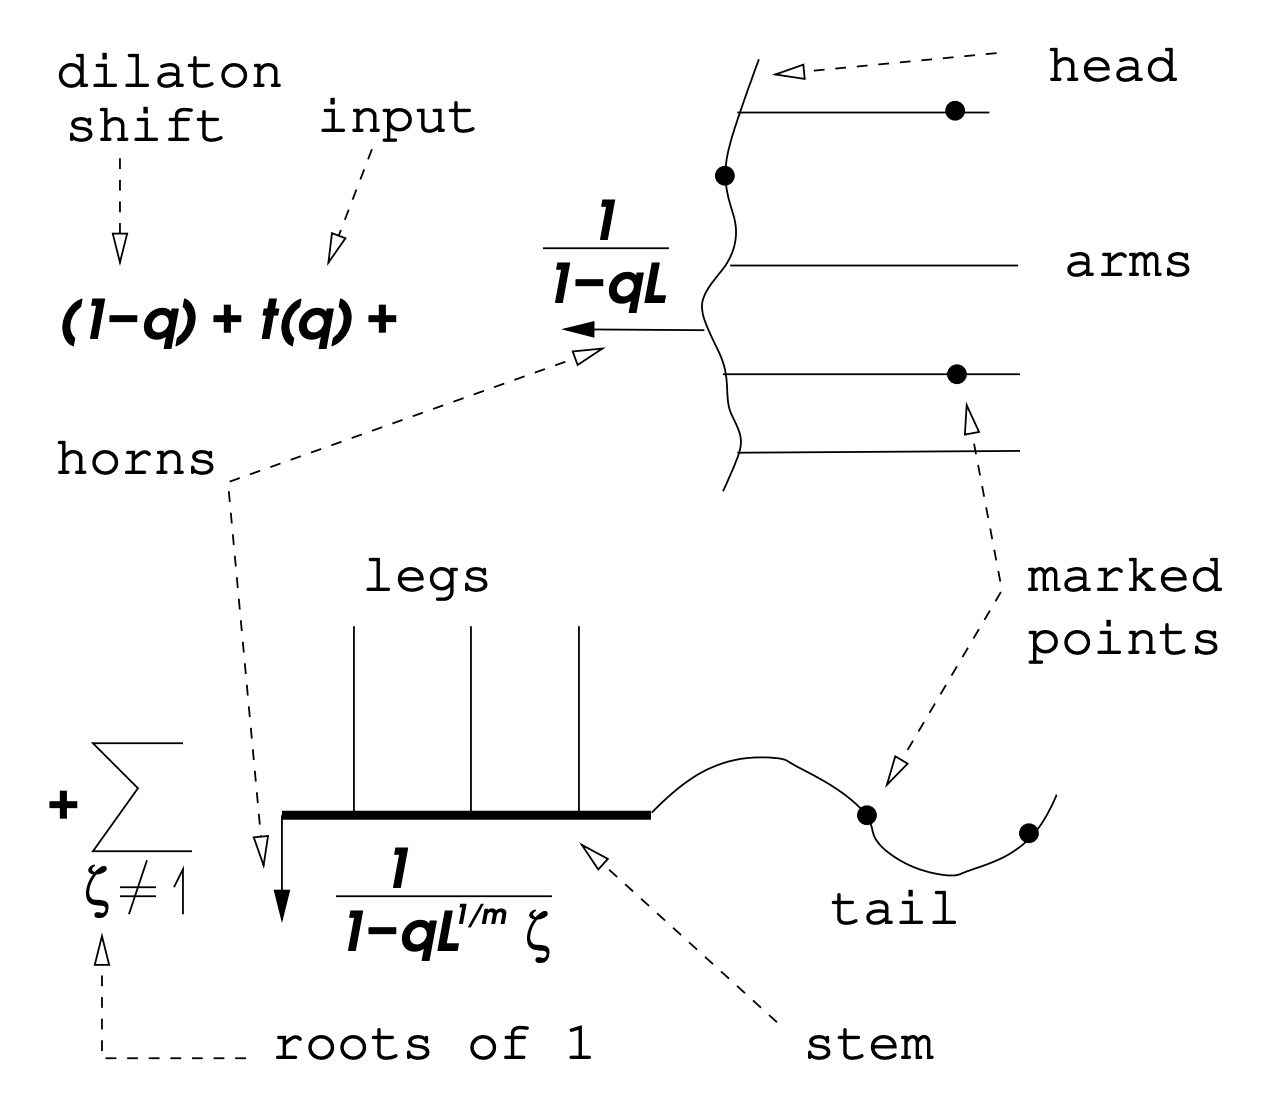
\includegraphics[width=0.8\textwidth]{givental.png}
    \caption{由 Givental-Tonita 给出的追踪惰性叠分支的一种方法。}
    \label{fig:givental-png}
\end{figure}

\begin{figure}[htpb]
    \centering
    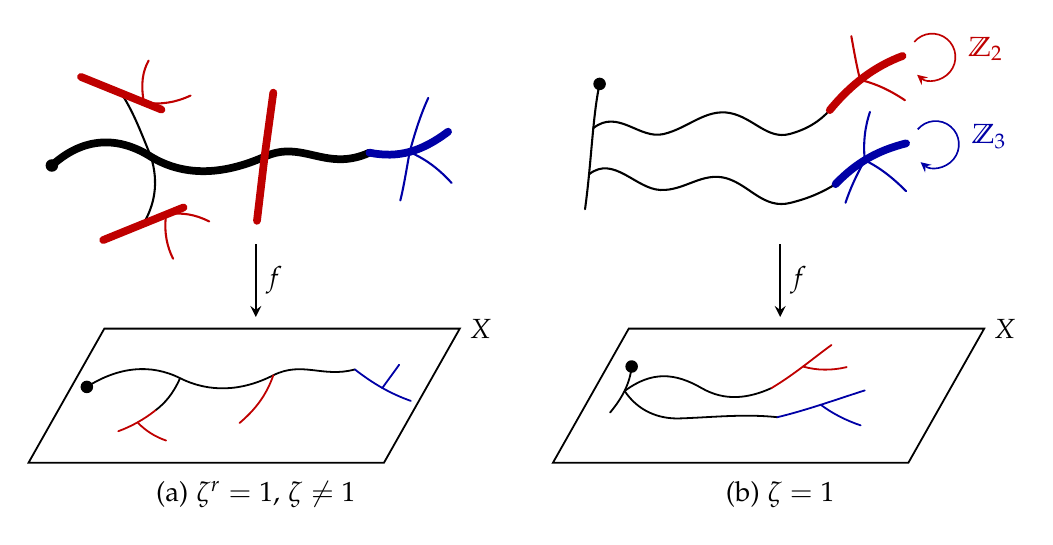
\begin{tikzpicture}[
        x=.74cm, y=.74cm,
        % Components of the domain curve. A cover style means the component
        % is a multiple cover of its image, drawn thick.
        dom/.style      ={black,         line width=.75pt, line cap=round},
        domcover/.style ={black,         line width=2.8pt, line cap=round},
        redcover/.style ={red!75!black,  line width=2.8pt, line cap=round},
        redtwig/.style  ={red!75!black,  line width=.75pt, line cap=round},
        bluecover/.style={blue!65!black, line width=2.8pt, line cap=round},
        bluetwig/.style ={blue!65!black, line width=.75pt, line cap=round},
        % Everything downstairs in X is drawn thin.
        img/.style      ={black,         line width=.65pt, line cap=round},
        redimg/.style   ={red!75!black,  line width=.65pt, line cap=round},
        blueimg/.style  ={blue!65!black, line width=.65pt, line cap=round},
        grparrow/.style ={->, >=stealth, line width=.6pt},
        fmap/.style     ={->, >=stealth, line width=.75pt},
        bull/.style     ={circle, fill=black, inner sep=1.6pt},
    ]

    %%%%%%%%%%%%%%%%%%%%%%%%%%%%%%%%%%%%%%%%%%%%%%%%%%%%%%%%%%%%%%%%%%%%%%%
    %% (a) zeta a primitive r-th root of unity, r >= 2.
    %%%%%%%%%%%%%%%%%%%%%%%%%%%%%%%%%%%%%%%%%%%%%%%%%%%%%%%%%%%%%%%%%%%%%%%
    \begin{scope}
        % The distinguished component: here g^r acts trivially on it, but g
        % does not, so it is a multiple cover of its image.
        \node[bull] at (-3.5,1.9) {};
        \draw[domcover]
            (-3.5,1.9)
            .. controls (-2.95,2.40) and (-2.35,2.40) .. (-1.80,2.05)
            .. controls (-1.25,1.72) and (-0.60,1.72) .. ( 0.15,2.05)
            .. controls ( 0.80,2.35) and ( 1.20,1.78) .. ( 1.95,2.12);

        % A leg meeting the distinguished component at a balanced node,
        % sticking out on both sides.  Each end carries a red multiple cover
        % together with the two branches interchanged by its automorphism.
        \draw[dom] (-1.80,2.05) .. controls (-2.00,2.55) and (-2.12,2.85) .. (-2.31,3.14);
        \draw[redcover] (-3.00,3.42) -- (-1.62,2.86);
        \draw[redtwig] (-1.92,2.98) .. controls (-1.98,3.30) and (-1.94,3.52) .. (-1.84,3.70);
        \draw[redtwig] (-1.92,2.98) .. controls (-1.62,2.94) and (-1.38,2.98) .. (-1.12,3.10);

        \draw[dom] (-1.80,2.05) .. controls (-1.66,1.60) and (-1.74,1.22) .. (-1.93,0.90);
        \draw[redcover] (-2.62,0.62) -- (-1.24,1.18);
        \draw[redtwig] (-1.54,1.06) .. controls (-1.58,0.74) and (-1.52,0.50) .. (-1.42,0.30);
        \draw[redtwig] (-1.54,1.06) .. controls (-1.26,1.10) and (-1.04,1.06) .. (-0.80,0.94);

        % A second balanced node, where the two legs are themselves the
        % multiple covers.
        \draw[redcover] (0.15,2.05) -- (0.30,3.15);
        \draw[redcover] (0.15,2.05) -- (0.02,0.95);

        % The tail: the part cut off at the unbalanced node.
        \draw[bluecover]
            (1.95,2.12) .. controls (2.45,2.02) and (2.85,2.14) .. (3.30,2.48);
        \draw[bluetwig] (2.64,2.13) .. controls (2.74,2.50) and (2.84,2.80) .. (2.96,3.06);
        \draw[bluetwig] (2.64,2.13) .. controls (2.58,1.80) and (2.54,1.54) .. (2.48,1.30);
        \draw[bluetwig] (2.64,2.13) .. controls (2.94,2.00) and (3.16,1.82) .. (3.36,1.60);

        \draw[fmap] (0,0.55) -- node[right] {$f$} (0,-0.70);

        % The target and the image of the map.
        \draw[img] (-3.9,-3.2) -- (2.2,-3.2) -- (3.5,-0.9) -- (-2.6,-0.9) -- cycle;
        \node[right] at (3.5,-0.9) {$X$};
        \node[bull] at (-2.90,-1.90) {};
        \draw[img] (-2.90,-1.90)
            .. controls (-2.35,-1.55) and (-1.80,-1.50) .. (-1.30,-1.75)
            .. controls (-0.80,-2.00) and (-0.25,-1.98) .. ( 0.30,-1.70)
            .. controls ( 0.80,-1.45) and ( 1.15,-1.75) .. ( 1.70,-1.60);
        % The two branches upstairs are folded onto the single one downstairs.
        \draw[img]    (-1.30,-1.75) .. controls (-1.42,-2.02) and (-1.56,-2.18) .. (-1.72,-2.30);
        \draw[redimg] (-1.72,-2.30) .. controls (-1.92,-2.46) and (-2.14,-2.58) .. (-2.36,-2.66);
        \draw[redimg] (-2.02,-2.52) .. controls (-1.88,-2.66) and (-1.72,-2.76) .. (-1.54,-2.82);
        \draw[redimg] ( 0.30,-1.70) .. controls ( 0.18,-2.05) and (-0.02,-2.30) .. (-0.28,-2.52);
        \draw[blueimg] (1.70,-1.60) .. controls (2.02,-1.85) and (2.32,-2.02) .. (2.66,-2.14);
        \draw[blueimg] (2.17,-1.92) .. controls (2.27,-1.78) and (2.36,-1.66) .. (2.46,-1.52);

        \node at (0,-3.75) {(a) \(\zeta^r = 1\), \(\zeta \neq 1\)};
    \end{scope}

    %%%%%%%%%%%%%%%%%%%%%%%%%%%%%%%%%%%%%%%%%%%%%%%%%%%%%%%%%%%%%%%%%%%%%%%
    %% (b) zeta = 1.
    %%%%%%%%%%%%%%%%%%%%%%%%%%%%%%%%%%%%%%%%%%%%%%%%%%%%%%%%%%%%%%%%%%%%%%%
    \begin{scope}[shift={(9,0)}]
        % Now g acts trivially on the distinguished component, so it is drawn
        % thin: it maps isomorphically onto its image.
        \node[bull] at (-3.10,3.30) {};
        \draw[dom] (-3.10,3.30) .. controls (-3.22,2.75) and (-3.24,1.95) .. (-3.35,1.15);
        \draw[dom] (-3.21,2.54)
            .. controls (-2.78,2.88) and (-2.42,2.34) .. (-2.00,2.44)
            .. controls (-1.58,2.54) and (-1.28,2.88) .. (-0.86,2.80)
            .. controls (-0.46,2.72) and (-0.22,2.34) .. ( 0.16,2.44)
            .. controls ( 0.46,2.52) and ( 0.68,2.66) .. ( 0.85,2.85);
        \draw[dom] (-3.28,1.75)
            .. controls (-2.86,2.08) and (-2.48,1.50) .. (-2.06,1.48)
            .. controls (-1.64,1.46) and (-1.34,1.80) .. (-0.92,1.68)
            .. controls (-0.52,1.56) and (-0.28,1.14) .. ( 0.18,1.26)
            .. controls ( 0.50,1.34) and ( 0.72,1.44) .. ( 0.95,1.58);

        % The arms: g acts nontrivially on them, through the indicated cyclic
        % group, which interchanges the thin branches sticking out.
        \draw[redcover] (0.85,2.85) .. controls (1.22,3.30) and (1.62,3.60) .. (2.10,3.78);
        \draw[redtwig] (1.37,3.37) .. controls (1.30,3.66) and (1.26,3.90) .. (1.22,4.12);
        \draw[redtwig] (1.37,3.37) .. controls (1.66,3.30) and (1.90,3.18) .. (2.14,3.02);
        \draw[grparrow, red!75!black]
            (2.30,4.02) arc[start angle=140, end angle=-130, radius=.40];
        \node[red!75!black, right] at (3.06,3.90) {$\Z_2$};

        \draw[bluecover] (0.95,1.58) .. controls (1.30,1.95) and (1.68,2.16) .. (2.16,2.28);
        \draw[bluetwig] (1.45,1.99) .. controls (1.42,2.32) and (1.46,2.58) .. (1.54,2.82);
        \draw[bluetwig] (1.45,1.99) .. controls (1.72,1.86) and (1.94,1.68) .. (2.16,1.46);
        \draw[bluetwig] (1.45,1.99) .. controls (1.30,1.72) and (1.20,1.50) .. (1.12,1.26);
        \draw[grparrow, blue!65!black]
            (2.36,2.52) arc[start angle=140, end angle=-130, radius=.40];
        \node[blue!65!black, right] at (3.12,2.40) {$\Z_3$};

        \draw[fmap] (0,0.55) -- node[right] {$f$} (0,-0.70);

        % The target and the image of the map.
        \draw[img] (-3.9,-3.2) -- (2.2,-3.2) -- (3.5,-0.9) -- (-2.6,-0.9) -- cycle;
        \node[right] at (3.5,-0.9) {$X$};
        \node[bull] at (-2.55,-1.55) {};
        \draw[img] (-2.55,-1.55) .. controls (-2.58,-1.85) and (-2.72,-2.10) .. (-2.92,-2.34);
        \draw[img] (-2.67,-1.97)
            .. controls (-2.20,-1.62) and (-1.80,-1.66) .. (-1.35,-1.92)
            .. controls (-0.95,-2.15) and (-0.55,-2.10) .. (-0.15,-1.92);
        \draw[img] (-2.67,-1.97)
            .. controls (-2.45,-2.30) and (-2.10,-2.46) .. (-1.70,-2.44)
            .. controls (-1.15,-2.42) and (-0.60,-2.36) .. (-0.05,-2.42);
        % Each arm is folded onto a single image curve with one branch.
        \draw[redimg] (-0.15,-1.92) .. controls (0.25,-1.68) and (0.55,-1.42) .. (0.88,-1.18);
        \draw[redimg] ( 0.39,-1.55) .. controls (0.63,-1.62) and (0.89,-1.62) .. (1.14,-1.56);
        \draw[blueimg] (-0.05,-2.42) .. controls (0.45,-2.30) and (0.95,-2.12) .. (1.45,-1.96);
        \draw[blueimg] ( 0.70,-2.21) .. controls (0.90,-2.36) and (1.14,-2.48) .. (1.38,-2.56);

        \node at (0,-3.75) {(b) \(\zeta = 1\)};
    \end{scope}
    \end{tikzpicture}
    \caption{\(I\bar{M}_{0,1}(X,\beta)\) 的各个分支，由周祐正给出。}
    \label{fig:adelic-components}
\end{figure}

下面我们来解释~\Cref{fig:adelic-components}。设 \(L_1\) 为第一标记点处的余切线，\(g\) 为 \(I\bar{M}_{0,1}(X,\beta)\) 中一点的自同构。则 \(\zeta\) 由如下条件定义：\(g\) 在 \(L_1\) 上的作用以 \(\zeta\) 为特征值。在两幅图中，圆点表示第一标记点及其在 \(X\) 中的像，而粗分支表示它是其像的多重覆盖。

首先设 \(\zeta = 1\)。此时黑色分支是包含第一标记点、且 \(g\) 在其上作用为恒同的最大连通分支。红色与蓝色分支恰是 \(g\) 在其上非平凡作用的那些分支，我们称之为\textit{臂}（arm）。

现在设 \(\zeta\) 是某个 \(r \geq 2\) 次单位根。此时黑色分支的结点关于 \(g\)-作用必须是平衡的，于是我们切去非平衡的部分（图中以蓝色标出），称之为\textit{尾}（tail）。在剩下的部分中，黑色分支是包含第一标记点、且 \(g^r\) 在其上作用为恒同的最大连通分支。最后，在去掉黑色分支和尾之后，我们称其余分支为\textit{腿}（leg）。

% \begin{figure}[htpb]
%     \centering
%     \resizebox{\textwidth}{!}{%
%     \begin{tikzpicture}[
%         x=1cm,
%         y=1cm,
%         curve/.style={black, line width=1.25pt, line cap=round},
%         fixed component/.style={black, line width=3.2pt, line cap=round},
%         red component/.style={red!75!black, line width=3.2pt, line cap=round},
%         blue component/.style={blue!70!black, line width=3.2pt, line cap=round},
%         image curve/.style={black, line width=1.05pt, line cap=round},
%         action arrow/.style={->, >=stealth, line width=.75pt},
%         map arrow/.style={->, >=stealth, line width=.8pt},
%         marked point/.style={circle, fill=black, inner sep=1.8pt}
%     ]
%         % The case of a nontrivial r-th root of unity.
%         \begin{scope}[xshift=0cm]
%             \node[font=\large] at (0,5.95)
%                 {$r\geq 2,\qquad \zeta^r=1,\quad \zeta\neq 1$};
%
%             % Domain curve.
%             \node[marked point] (p1) at (-3.15,3.7) {};
%             \draw[fixed component]
%                 (p1) .. controls (-2.25,4.15) and (-1.55,4.2) ..
%                 (-1.15,3.92)
%                 .. controls (-0.55,3.45) and (0.35,3.45) ..
%                 (0.85,3.82)
%                 .. controls (1.35,3.35) and (1.85,3.45) ..
%                 (2.2,4.05);
%             \fill (-1.15,3.92) circle (2.2pt);
%             \fill (0.85,3.82) circle (2.2pt);
%             \fill (2.2,4.05) circle (2.2pt);
%
%             % Two legs attached to balanced nodes.
%             \draw[curve]
%                 (-1.15,3.92) .. controls (-1.25,4.45) and (-1.35,4.78) ..
%                 (-1.72,5.18);
%             \draw[red component]
%                 (-2.18,5.48) .. controls (-1.92,5.25) and (-1.65,5.08) ..
%                 (-1.36,5.02);
%             \draw[curve, red!75!black]
%                 (-1.67,5.14) .. controls (-1.64,5.35) and (-1.59,5.55) ..
%                 (-1.53,5.72);
%             \draw[curve, red!75!black]
%                 (-1.53,5.08) .. controls (-1.34,5.14) and (-1.18,5.25) ..
%                 (-1.02,5.4);
%             \draw[action arrow, red!75!black]
%                 (-1.9,5.38) arc[start angle=20,end angle=315,radius=.42];
%
%             \draw[curve]
%                 (-1.15,3.92) .. controls (-1.1,3.35) and (-1.25,3.0) ..
%                 (-1.62,2.63);
%             \draw[red component]
%                 (-2.18,2.32) .. controls (-1.9,2.56) and (-1.6,2.75) ..
%                 (-1.3,2.84);
%             \draw[curve, red!75!black]
%                 (-1.65,2.68) .. controls (-1.62,2.48) and (-1.59,2.25) ..
%                 (-1.54,2.06);
%             \draw[curve, red!75!black]
%                 (-1.5,2.76) .. controls (-1.31,2.7) and (-1.14,2.58) ..
%                 (-.98,2.42);
%             \draw[action arrow, red!75!black]
%                 (-1.85,2.57) arc[start angle=25,end angle=315,radius=.38];
%
%             % A second symmetric pair of balanced legs.
%             \draw[curve] (0.2,3.48) .. controls (0.16,4.05) and (0.2,4.35) ..
%                 (0.32,4.7);
%             \draw[red component] (0.2,3.9) -- (0.33,4.72);
%             \draw[curve] (0.2,3.48) .. controls (0.16,3.12) and (0.08,2.82) ..
%                 (-0.02,2.48);
%             \draw[red component] (0.11,3.05) -- (-0.03,2.46);
%
%             % The nonbalanced tail.
%             \draw[blue component]
%                 (2.2,4.05) .. controls (2.68,3.92) and (3.05,4.02) ..
%                 (3.48,4.3);
%             \draw[curve, blue!70!black] (2.86,4.08) -- (3.15,4.78);
%             \draw[curve, blue!70!black] (2.95,4.07) -- (2.88,3.35);
%             \draw[curve, blue!70!black] (2.95,4.07) -- (3.45,3.55);
%
%             % The target and the image of the map.
%             \draw[curve]
%                 (-3.55,-1.65) -- (2.48,-1.65) -- (3.48,1.0) --
%                 (-2.65,1.0) -- cycle;
%             \node[marked point] (xp1) at (-2.65,-0.25) {};
%             \draw[image curve]
%                 (xp1) .. controls (-2.05,0.04) and (-1.55,.22) ..
%                 (-1.15,.12)
%                 .. controls (-.5,-.05) and (-.2,-.1) ..
%                 (.12,.18)
%                 .. controls (.55,.55) and (1.0,.62) ..
%                 (1.55,.45);
%             % The first red orbit maps to a black connector followed by
%             % one red image curve; its two thin branches fold to the
%             % smaller red branch.
%             \draw[image curve]
%                 (-1.15,.12) .. controls (-1.23,-.08) and (-1.34,-.23) ..
%                 (-1.48,-.32);
%             \draw[red!75!black, line width=1.05pt, line cap=round]
%                 (-1.48,-.32) .. controls (-1.62,-.45) and (-1.78,-.58) ..
%                 (-1.92,-.65);
%             \draw[red!75!black, line width=1.05pt, line cap=round]
%                 (-1.69,-.51) .. controls (-1.58,-.64) and (-1.45,-.72) ..
%                 (-1.31,-.76);
%             \draw[red!75!black, line width=1.05pt, line cap=round]
%                 (.12,.18) .. controls (.02,-.22) and (-.25,-.38) ..
%                 (-.48,-.63);
%             \draw[blue!70!black, line width=1.05pt, line cap=round]
%                 (1.05,.57) .. controls (1.35,.12) and (1.68,-.18) ..
%                 (2.08,-.38);
%             \draw[blue!70!black, line width=1.05pt, line cap=round]
%                 (1.78,-.2) .. controls (1.82,-.08) and (1.88,.04) ..
%                 (1.96,.15);
%             \draw[map arrow] (0,2.62) -- node[right] {$f$} (0,1.22);
%             \node at (0,-2.1) {$(a)\ \zeta\neq 1$};
%         \end{scope}
%
%         % The untwisted eigenvalue case.
%         \begin{scope}[xshift=8.25cm]
%             \node[font=\large] at (0,5.95)
%                 {$I\overline{\mathcal M}_{0,1}(X,\beta),\qquad
%                   \on{Tr} g|_{L_1}=\zeta$};
%
%             % Domain curve: the thick portions have multiple covers onto
%             % their images.
%             \node[marked point] (p2) at (-2.95,4.45) {};
%             \draw[fixed component]
%                 (p2) .. controls (-3.08,3.85) and (-3.08,3.18) ..
%                 (-3.18,2.65);
%             \draw[curve]
%                 (-3.02,3.9) .. controls (-2.42,4.05) and (-2.0,3.62) ..
%                 (-1.62,3.72)
%                 .. controls (-1.18,3.3) and (-.72,3.18) ..
%                 (-.2,3.32);
%             \draw[curve]
%                 (-3.13,3.25) .. controls (-2.6,3.52) and (-2.25,2.88) ..
%                 (-1.8,2.68)
%                 .. controls (-1.25,2.4) and (-.68,2.42) ..
%                 (-.15,2.48);
%
%             % Nontrivial arms, shown in red and blue.
%             \draw[curve]
%                 (-.2,3.32) .. controls (.3,3.48) and (.5,3.72) ..
%                 (.76,3.92);
%             \draw[red component]
%                 (.76,3.92) .. controls (1.1,4.42) and (1.5,4.72) ..
%                 (2.02,4.9);
%             \draw[curve, red!75!black]
%                 (1.12,4.4) .. controls (1.08,4.68) and (1.05,4.92) ..
%                 (1.02,5.18);
%             \draw[curve, red!75!black]
%                 (1.55,4.7) .. controls (1.82,4.62) and (2.04,4.48) ..
%                 (2.25,4.3);
%             \draw[action arrow, red!75!black]
%                 (1.6,4.88) arc[start angle=210,end angle=-35,radius=.48];
%             \node[red!75!black, left] at (1.02,5.08) {$\Z_2$};
%
%             \draw[curve]
%                 (-.15,2.48) .. controls (.28,2.45) and (.55,2.64) ..
%                 (.86,2.76);
%             \draw[blue component]
%                 (.86,2.76) .. controls (1.18,3.13) and (1.52,3.32) ..
%                 (2.0,3.42);
%             \draw[curve, blue!70!black]
%                 (1.27,3.13) .. controls (1.34,3.4) and (1.43,3.65) ..
%                 (1.55,3.9);
%             \draw[curve, blue!70!black]
%                 (1.57,3.33) .. controls (1.83,3.2) and (2.05,3.02) ..
%                 (2.27,2.82);
%             \draw[action arrow, blue!70!black]
%                 (1.9,3.37) arc[start angle=145,end angle=-120,radius=.43];
%             \node[blue!70!black, above] at (2.55,3.62) {$\Z_3$};
%
%             % Target X and the images of the colored components.
%             \draw[curve]
%                 (-3.55,-1.65) -- (2.48,-1.65) -- (3.48,1.0) --
%                 (-2.65,1.0) -- cycle;
%             \node[marked point] (xp2) at (-2.05,.02) {};
%             \draw[image curve]
%                 (xp2) .. controls (-2.0,-.32) and (-2.35,-.62) ..
%                 (-2.62,-.93);
%             \draw[image curve]
%                 (-2.25,-.52) .. controls (-1.82,-.12) and (-1.55,-.12) ..
%                 (-1.14,-.42)
%                 .. controls (-.88,-.62) and (-.54,-.63) ..
%                 (-.22,-.52);
%             \draw[image curve]
%                 (-2.25,-.52) .. controls (-2.58,-.44) and (-2.75,-.62) ..
%                 (-2.98,-.83);
%             \draw[red!75!black, line width=1.05pt]
%                 (-.22,-.52) .. controls (.22,-.13) and (.5,.22) ..
%                 (.82,.48);
%             % The two thin red branches upstairs fold to this one
%             % additional branch of the red image curve.
%             \draw[red!75!black, line width=1.05pt, line cap=round]
%                 (.345,.029) .. controls (.57,-.02) and (.77,.06) ..
%                 (1.0,.18);
%             % A chain of black components joins the blue image to the
%             % distinguished black component.
%             \draw[image curve]
%                 (-2.25,-.52) .. controls (-2.12,-.76) and (-2.0,-.91) ..
%                 (-1.88,-1.0);
%             \draw[image curve]
%                 (-1.88,-1.0) .. controls (-1.76,-.82) and (-1.53,-.91) ..
%                 (-1.38,-1.18);
%             \draw[image curve]
%                 (-1.38,-1.18) .. controls (-.65,-.76) and (.08,-.68) ..
%                 (.78,-.72);
%             \draw[blue!70!black, line width=1.05pt, line cap=round]
%                 (.78,-.72) .. controls (1.24,-.74) and (1.58,-.62) ..
%                 (1.98,-.32);
%             \draw[map arrow] (0,2.03) -- node[right] {$f$} (0,1.22);
%             \node at (0,-2.1) {$(b)\ \zeta=1$};
%         \end{scope}
%     \end{tikzpicture}%
%     }
%     \caption{The decomposition of a component of
%     \(I\overline{\mathcal M}_{0,1}(X,\beta)\) into its distinguished
%     component, legs or arms, and tail, provided by You-Cheng. Thick curves indicate components
%     that map with degree greater than one onto their images. Symmetric
%     branches occur on the domain, and \(f\) folds each orbit to a single
%     image curve in \(X\).}
%     \label{fig:adelic-components}
% \end{figure}
%
% We will now explain the meaning of the different parts of~\Cref{fig:adelic-components}. Let \(L_1\)
% be the cotangent line at the first marked point and define \(\zeta\) by
% \[
%     g|_{L_1}=\zeta\,\mr{Id}_{L_1}.
% \]
% The bullets denote the first marked point and its image in \(X\), and a
% thick curve denotes a component that is a multiple cover of its image.
% The black component is the maximal connected component containing the
% first marked point on which \(g\) acts trivially when \(\zeta=1\). The red
% and blue components on which \(g\) acts nontrivially are called
% \textit{arms}.
%
% More generally, suppose that \(\zeta\) is an \(r\)-th root of unity with
% \(r\geq 2\). The nodes of the thick black component must be balanced with
% respect to the \(g\)-action. Cut off the part attached at an unbalanced
% node (the blue component in the figure); this part is called the
% \textit{tail}. In what remains, the thick black component is the maximal
% connected component containing the first marked point on which \(g^r\)
% acts trivially. After removing the black component and the tail, the
% remaining components are called \textit{legs}.

下述定义属于 Givental。我们记
\[ \ab<\frac{\Phi}{1-qL}>_{0,1,\beta}^{X,K} \coloneqq \sum_{\zeta} \ab<\frac{\Phi}{1-qL}>_{0,1,\beta}^{X_{\zeta}}, \]
其中 \(X_{\zeta}\) 项就是在黎曼--罗赫定理下 \(M_{\zeta}\) 的贡献。现在我们来定义臂、腿和尾。这里定义\textit{臂}
\[ \mr{arm}(q) \coloneqq \sum_{\beta, \alpha, \zeta \neq 1} Q^{\beta} \Phi^{\alpha}\ab<\frac{\Phi_{\alpha}}{1-qL}>_{0,1,\beta}^{X_{\zeta}}, \]
\textit{腿}
\[ \mr{leg}_{\zeta}(q) \coloneqq \mr{leg}_r(q) = \Psi^r (\mr{arm}(q)), \]
以及\textit{尾}
\[ \mr{tail}_{\zeta}(q) \coloneqq \sum_{\beta, \alpha, \zeta' \neq \zeta} Q^{\beta} \Phi^{\alpha} \ab<\frac{\Phi_{\alpha}}{1-qL}>_{0,1,\beta}^{X_{\zeta'}}. \]

\begin{prop}[{\cite{GiventalTonita2014}}]
    J-函数在 \(q = 1\) 处的洛朗展开由下式给出
    \begin{align*}
        J^K(0)_{q=1} &= J^{\mr{fake}}(\mr{arm}(q)) \\
        &\coloneqq 1-q + \mr{arm}(q) + \sum_{n,\beta,\alpha} \frac{Q^{\beta}\Phi^{\alpha}}{n!} \ab<\frac{\Phi_{\alpha}}{1-qL}, \mr{arm}(L), \ldots, \mr{arm}(L)>_{0,n+1,\beta}^{\mr{fake}},
    \end{align*}
    其中伪不变量（fake invariants）由黎曼--罗赫定理算出，且仅考虑未扭扇区的贡献。
\end{prop}

\begin{prop}[{\cite{GiventalTonita2014}}]
    在任意其他单位根 \(\zeta \neq 1\) 处，我们有
    \begin{align*}
        &J^K(0)_{q = \zeta} = (1-q) + \mr{tail}_{\zeta}(q) \\
        &+ \sum_{n,\beta,\alpha} \frac{Q^{r\beta}\Phi^{\alpha}}{n!} \ab[\frac{\Phi_{\alpha}}{1-\zeta q L^{1/r}}, \mr{leg}_r(L), \ldots, \mr{leg}_r(L), 1 - \zeta^{-1}L^{1/r} + \mr{tail}_{\zeta}(\zeta^{-1} L^{1/r})]^{\mr{stem}},
    \end{align*}
    其中茎（stem）是 \(X \times B\mu_r\) 的某个伪不变量，定义在如下模空间上
    \[ \bar{M}_{0,n+2,\beta}^X(\zeta) \coloneqq \bar{M}_{0,n+2}(X \times B\mu_r, \beta, (g, 1, \ldots, 1, g^{-1})). \]
    它由如下公式定义
    \begin{align*}
        [\cdots]^{\mr{stem}} \coloneqq \int_{[\bar{M}_{0,n+2,\beta}^X(\zeta)]^{\vir}} \on{td}(T_{\bar{M}}) \on{ch}\ab(\frac{\on{Tr}(\cdots)}{\on{Tr}(\lambda_{-1}(N^*))}), 
    \end{align*}
    其中 \(N\) 表示 \(\bar{M}_{0,n+2,\beta}^X(\zeta) \subset \bar{M}_{0,nr+2}(X, r\beta)\) 的法丛。
\end{prop}

\begin{rmk}
    如果我们能计算伪（fake）理论与茎（stem）理论，那么就能计算亏格零量子 K 不变量。
\end{rmk}


\subsection{点的量子 K 理论}%
\label{sub:Quantum K-theory of a point}

一个自然的问题是研究高亏格量子 K理论。我们从最简单的目标，即一个点，开始。研究高亏格的一个动机是尝试证明 Calabi-Yau 四维簇的 Klemm-Pandharipande 定义的 GV 不变量或 Calabi-Yau 五维簇的 Pandharipande-Zinger 定义的 GV 不变量的整性（在这种情形下，我们只需考虑亏格 \(1\)）。我们需要考虑点的量子 K理论的一个原因在于，在 \(I\bar{M}_{1,1}(X, \beta)\) 中，存在一些连通分支，其中整条亏格 \(1\) 的曲线被收缩为一点。

\begin{quest}
    K理论版本的 Witten-Kontsevich 定理是什么？\footnote{据周祐正说，困难无处不在。}
\end{quest}

我们先回顾上同调版本的 Witten 猜想。我们从算子
\[ L = \partial_x^2 + u(x) \]
出发，并将其形变为
\[ \tilde{L} = \partial_x^2 + u(x, T_3, T_5, \ldots), \]
其中我们应将 \(x = T_1\) 且 \(u(x) = u(x, 0, 0,\ldots)\)。形式地，利用性质
\[ \partial^n \circ f = \sum_{m = 0}^{\infty} \binom{n}{m} f^{(m)} \partial^{n-m} \]
（对所有整数 \(n \in \Z\) 成立），将 \(L^{1/2}\) 写成
\[ L^{1/2} = \partial_x + \sum_{k > 0} a_{-k}(x) \partial_x^{-k}. \]
特别地，我们由方程
\[ \pdv{\tilde{L}}{T_{2k+1}} = \ab[(\tilde{L}^{\frac{2k+1}{2}})_{\geq 0}, \tilde{L}] \]
（对所有 \(k \geq 0\)）构造（2-）KdV 族。我们把满足
\[ 2 \pdv[2]{}{x}\log \tau(x, T_3, T_5, \ldots) = u(x, T_3, T_5, \ldots) \]
的函数 \(\tau\) 称为 \textit{\(\tau\)-函数}。现在用 \(u = 2x\) 进行上述过程。定义函数
\[ F(t_0, t_1, \ldots) \coloneqq \sum_{n \geq 0} \sum_{k_0, \ldots, k_n} \ab<\tau_0^{k_0} \cdots \tau_n^{k_n}> \frac{t_0^{k_0} \cdots t_n^{k_n}}{k_0! \cdots k_n!}. \]
注意到由于亏格完全由插入的个数和插入的次数决定，记号
\[ \ab<\tau_0^{k_0} \cdots \tau_n^{k_n}> \]
唯一确定了一个点的后代 GW 不变量。

\begin{thm}[Kontsevich {\cite{Kontsevich1992}}]
    \(F\) 是从 \(L = \partial_x^2 + 2x\) 出发构造的 KdV 族的 \(\tau\)-函数，其中变量替换为 \(t_i = (2i+1)!! T_{2i+1}\)。
\end{thm}

这个定理的一个应用是考虑虚局部化。例如，假设我们考虑 \(\bar{M}_{g,0}(X, d[C])\)，其中 \(C\) 是 Calabi-Yau 三维簇中唯一的有理曲线，法丛为 \(N = \mc{O}(-1)\oplus \mc{O}(-1)\)。那么在此设定下我们可以化归到局部模型，并通过虚局部化计算
\begin{align*}
    \int_{[\bar{M}_{g,0}(\P^1, d)]^{\vir}} c_{\mr{top}}(R^1 \pi_* N) = \sum_{m \vdash d} \frac{(-1)^{d-L(m)}}{\abs{\Aut(m)}} \int_{\bar{M}_{g, L(m)}} \frac{1 + \cdots + c_g(\mc{H})}{\prod_i (1-m_i \psi_i)}
\end{align*}
。如果我们希望在 K理论中得到类似的结果，那么就需要考虑形如
\[ \chi\ab(\bar{M}_{g, L(m)}/\Aut(m), \frac{\lambda_{-1}(\mc{H})}{1-m_i L_i}) \]
的项，因此我们需要考虑点的置换等变量子 K理论。

下面我们进行文献综述。首先，Lee~\cite{Lee1997} 计算了公式
\[ \ab<\frac{1}{1-q_1 L}, \ldots, \frac{1}{1-q_n L}>_{0,n}^{\mr{pt}, K} = \ab(\prod_{i=1}^n \frac{1}{1-q_i}) \ab(1 + \sum_{i=1}^n \frac{q_i}{1-q_i})^{n-3}. \]
后来，Lee--Qu~\cite{LeeQu2014} 给出了一种原则上计算
\[ \ab<\frac{1}{1-q_1 L}, \ldots, \frac{1}{1-q_n L}>_{1,n}^{\mr{pt}, K} \]
的方法。Givental~\cite{Givental2017K1} 计算了公式
\[ \sum_{n \geq 2} \ab<\frac{1}{1-q L}, 1, \ldots, 1>_{0,1+n}^{S_n} = (1-q) \exp\ab(\sum_{k > 0} \frac{\Psi^k}{k} \ab(1 + \frac{q}{1-q})). \]
最后，Milanov~\cite{Milanov2025} 在一份 2024 年首次公开的预印本中计算了
\begin{align*}
    \sum_{n \geq 0}& \ab<\frac{1}{1-q_1 L}, \ldots, \frac{1}{1-q_r L}, 1, \ldots, 1>_{0,r+n}^{S_n} \\
    &= \ab(\prod_{i=1}^{r} \frac{1}{1-q_i})\ab(1 + \sum_{i=1}^r \frac{q_i}{1-q_i}) \exp\ab(\sum_{k > 0} \frac{\Psi^k}{k} \ab(1 + \sum_{i=1}^r \frac{q_i}{1-q_i})). 
\end{align*}

以下多重霍奇递推以及基于它们的新的亏格一计算出自周祐正，并在本讲中给出。

设 \(s \in \Z\)，定义多重霍奇层 \(\mc{H}_s \coloneqq R^0 \pi_* (\omega_{\pi}^s)\)。考虑映射 \(\bar{M}_{g,n+1} \xrightarrow{\pi} \bar{M}_{g,n}\)，我们将上方的余切线记为 \(L_i\)，下方的记为 \(\ell_i\)。

\begin{lem}
    对所有整数 \(s\) 和 \(d_i\)，我们有
    \[ \pi_*\ab(\omega_{\pi}^s\ab(\sum_{i=1}^n d_i D_i)) = \mc{H}_s-\mc{H}_{1-s}^* + \sum_{i=1}^n \sum_{k=1}^{d_i} \ell_i^{-k+s}. \]
\end{lem}

\begin{rmk}
    注意到若 \(f(q) \in \Z[q]\)，则 \(\exp \sum_k \frac{\Psi^k}{k} (f(q)) \in \Z \ps{q}\)。原因在于这一运算把 \(f = \sum_{i=1}^{n} a_i q^i\) 映为 \(\prod_{i=1}^n \frac{1}{(1-q^i)^{a_i}}\)。
\end{rmk}

\begin{proof}
    当所有 \(d_i\) 都为零时，由 Serre 对偶我们看到
    \[ R^0 \pi_* \omega_{\pi}^s - R^1 \pi_* \omega_{\pi}^s = \mc{H}_s - \mc{H}_{1-s}^* \]
    。下一步是证明
    \[ \pi_* \omega_{\pi}^s ((r+1)D_i) = \pi_* \omega_{\pi}^s(r D_i) + \ell_i^{s-r-1}. \]
    这里我们先考虑正合列
    \[ 0 \to \mc{O} (-D_i) \to \mc{O} \to \mc{O}_{D_i} \to 0 \]
    并用 \(\omega_{\pi}^s\) 扭变得到
    \[ 0 \to \omega_{\pi}^s(r D_i) \to \omega_{\pi}^s ((r+1)D_i) \to \omega_{\pi}^s ((r+1)D_i) \otimes \mc{O}_{D_i} \to 0 \]
    ，然后计算前推。
\end{proof}

\begin{lem}
    设 \(f_i\) 为有理函数，例如 \(\frac{1}{1-q L}\)。则
    \begin{align*}
        \ab<f_1(L), \ldots, f_n(L), L_{n+1}^r>_{g, n+1} ={}& \sum_{i=1}^n \ab<f_1(L), \ldots, D(f_i f_{n+1}), \ldots, f_n(L)>_{g, n} \\
        &+ \ab<f_1(L), \ldots, f_n(L) \mid \mc{H}_r - \mc{H}_{1-r}^*>_{g,n},
    \end{align*}
    其中 \(f_{n+1} = L_{n+1}^r\)，且 \((Df)(x) \coloneqq \frac{f(x)-f(1)}{x-1}\)。
\end{lem}

为证明这一点，我们需要考虑前推
\begin{align*}
    \pi_* (L_1^{d_1} \cdots L_{n+1}^{d_{n+1}}) &= \pi_* \ab(\pi^*(\ell_1^{d_1} \otimes \cdots \otimes \ell_n^{d_n}) \otimes \omega_{\pi}^{d_{n+1}}\ab(\sum_i (d_i+d_{n+1})D_i)).
\end{align*}
这里我们用到 \(L_i = (\pi^* \ell_i)(D_i)\) 与 \(L_{n+1} = \omega_{\pi}(D_1 + \cdots + D_n)\) 这两个事实。应用上一个引理，我们看到前推变为
\[ (\ell_1^{d_1} \cdots \ell_n^{d_n})\ab(\mc{H}_{d_{n+1}} - \mc{H}_{1-d_{n+1}}^* + \sum_{i=1}^n \sum_{k=1}^{d_i + d_{n+1}} \ell_i^{-k+d_{n+1}}). \]
现在，Lee 的公式通过展开式
\[ \frac{1}{1-qL} = \frac{1}{1-q} \sum_{k \geq 0} \frac{q^k(L-1)^k}{(1-q)^k} \]
计算关联子
\[ \ab<(L-1)^{k_1}, \ldots, (L-1)^{k_n}>_{0,n} = \frac{(n-3)!}{\prod_{i=1}^n k_i! \ab(n-3-\sum_i k_i)!} \]
。这里注意在亏格 \(0\) 没有霍奇丛，因此实际上可以用该引理导出 Lee 的公式。

\begin{lem}
    我们有
    \[ \mc{H}_r - \mc{H}_{1-r}^* = \pi^* (\mc{H}_r - \mc{H}_{1-r}^*) - \sum_{i=1}^n (D^2 (\pi^* \ell_i)^r) \mc{O}_{D_i}. \]
\end{lem}

这些引理合起来表明，我们可以化归到只有一个标记的情形，代价是插入项变得非常复杂，并且处处引入多重霍奇项。在亏格 \(1\)，事情变得容易，因为在 \(\bar{M}_{1,1}\) 上我们有
\[ \mc{H}_r = \mc{O}(r) = L_1^r. \]
此时，回顾经典公式
\[ \chi\ab(\bar{M}_{1,1}, \frac{1}{1-qL}) = \frac{1}{(1-q^4)(1-q^6)}. \]
遗憾的是，计算
\[ \chi\ab(\bar{M}_{1,n}; \frac{1}{1-q_1 L} \cdots \frac{1}{1-q_n L}) \]
太困难了，因此我们可以尝试计算
\[ \chi\ab(\bar{M}_{1,1}; \frac{1}{1-q_1 L_1} \cdots \frac{1}{1-q_n L_1})  \]
，这是已知的，但目前还不清楚如何为它写出一个好的公式。考虑它的原因在于运算
\[ \Z\ps{q} \xrightarrow{[]_r} \Z\ps{q_1, \ldots, q_r} \qquad q^k \to h_k(q_1, \ldots, q_r) \coloneqq \sum_{\ell_1 + \cdots + \ell_r = k} q_1^{\ell_1} \cdots q_r^{\ell_r}. \]
遗憾的是，周祐正不知道如何以好的形式写出
\[ \chi\ab(\bar{M}_{1,1}; \frac{1}{1-q_1 L_1} \cdots \frac{1}{1-q_n L_1}) = \ab[\frac{1}{(1-q^4)(1-q^6)}]_n \]
。原则上我们可以写出形如
\[ [f(q)]_2 \coloneqq \frac{q_1 f(q_1) - q_2 f(q_2)}{q_1 - q_2} \]
的公式，但这似乎帮助不大。

\subsection{点的置换等变理论}%
\label{sub:Permutation-equivariant theory of a point}

我们可以用另一种方式计算 \(\chi\ab(\bar{M}_{1,1}, \frac{1}{1-q L})\)。考虑椭圆曲线上的对合，它给出一个映射
\[ \bar{M}_{1,1} \to \bar{M}_{0,1+3}/S_3. \]
于是，Givental~\cite{Givental2017K1} 计算出
\[ \chi\ab([\bar{M}_{0,1+n-1}/S_{n-1}], \frac{1}{1-qL}) = \prod_{i=2}^{n-1} \frac{1}{1-q^i}. \]
特别地，我们得到
\[ \frac{1}{(1-q^2)(1-q^3)}, \]
又因为该映射是一个 \(\mu_2\)-gerbe（或在对象层面是 \(2:1\) 覆叠），我们就得到了所要的公式。

考虑 \(\mc{H}_{g,1} \subset \bar{M}_{g,1}\) 为超椭圆轨迹。注意标记落在一个 Weierstrass 点上。注意超椭圆对合的不动点被映到 \(\P^1\) 上的 \(2g+1\) 个点，因此人们会希望用计算
\[ \chi\ab(\bar{M}_{0,1+2g+1}/S_{2g+1}, \frac{1}{1-q L}) = \prod_{i=2}^{2g+1} \frac{1}{1-q^i} \]
来计算量
\(\chi\ab(\mc{H}_{g,1}, \frac{1}{1-qL})\)。然而，由于上方曲线的退化方式，我们需要考虑最后 \(2g+1\) 个标记权重为 \(\frac{1}{2}\) 的 Hassett 模空间~\cite{Hassett2003}。
 







\section{拟映射越墙（周杨）}%
\label{sec:Quasimap wall-crossing (Yang Zhou)}

本讲中的主要越墙（wall-crossing）定理与主空间构造来自~\cite{Zhou2022}。更早的亏格零与高亏格结果见~\cite{CFK2014,CFK2020}，稳定拟映射（quasimap）的基础则见~\cite{CFKM2014}。

设 \(X\) 为五次三维簇。我们的目标是计数 \(X\) 上的亏格零曲线，这一问题已由 Givental 与 Lian-Liu-Yau 解决。通过闭浸入 \(X \subset \P^4\)，我们可以写出
\[ \bar{M}_0(X, d) \subset \bar{M}_0(\P^4, d), \]
它是光滑的，并带有 \((\C^{\times})^5\) 的环面作用。若一个映射在该作用下不动，则其定义域必然有一些分支映到不动点，另一些分支则构成 \(1\) 维轨道的 \(n :1\) 覆盖。特别地，不动点轨迹由一组图来标号。

在这一情形下，我们有量子 Lefschetz 原理，它断言
\[ [\bar{M}_0(X, d)]^{\on{vir}} = e(E) \cap [\bar{M}_0(\P^4, d)]. \]
这里向量丛 \(E\) 由
\[ E = \pi_* f^* \mc{O}(5), \]
定义，其中 \(\pi\) 是泛曲线，\(f\) 是泛稳定映射。我们将对下述结果给出另一种视角：若
\begin{align*}
    I(q, z) &= 1 + \sum_{d > 0} \frac{\prod_{k=1}^{5d} (5H+kz)}{\prod_{k=1}^d (H+kz)^5} q^d \in H^*(X)[z^{-1}] \ps{q} \\
    &= I_0(q) \cdot 1 + I_1(q) \frac{H}{z} + I_2(q) \frac{H^2}{z^2} + I_3(q) \frac{H^3}{z^3},
\end{align*}
则
\[ J (Q, z) = 1+ \sum_{d>0} \phi^{\alpha} \ab<\frac{\phi_{\alpha}}{z(z-\psi)}>_{0,1}^X Q^d = \frac{I}{I_0} \]
其中镜像变换为 \(Q = q \exp\ab(\frac{I_1}{I_0})\)。

\subsection{朴素计数}%
\label{sub:Naive counting}

我们将考虑从固定 \(\P^1\) 出发的“映射”\(\P^1 \to X \subset \P^4\)。为简单起见，设 \(X = \ab(\sum x_i^5 = 0)\) 为 Fermat 五次三维簇。它由一族 \([f_0, \ldots, f_4]\) 给出，其中 \(f_i \in \C[u,v]\) 满足 \(\deg f_i = d\) 且 \(\sum f_i^5 = 0\)。为了得到真正的态射，我们需要 \(f_i\) 没有公共零点，但这样得到的模空间不是真的（proper），因此我们放宽这一条件。于是我们考虑模空间
\[ QG(X, d) =  \ab\{ [f_0, \ldots, f_4] \middle\vert \Vectorstack{{ f_i \in \C[u,v] } { \deg f_i = d }}, \sum f_i^5 = 0, (f_0, \ldots, f_4) \neq (0,\ldots, 0) \} \bigg/ \C^{\times}. \]
它含于相应的模空间
\begin{align*}
    QG(\P^4, d) &\coloneqq  \ab\{ [f_0, \ldots, f_4] \mid f_i \in \C[u,v], \deg f_i = d, (f_0, \ldots, f_4) \neq (0, \ldots, 0) \} \\
    &\cong \P^{5d+5-1} 
\end{align*}
之中，后者参数化到射影空间的有理映射。这里有两个问题。其一，定义域也被参数化了，因此我们需要考虑 \(\P^1\) 的自同构。其二，为了得到稳定映射，我们需要对定义域作爆破。

首先，令 \(\C^{\times}\) 通过缩放 \(u\) 作用于 \(\P^1\)。考虑由下式定义的特殊不动点轨迹 \(F_{\star} \subset QG(X, d)\)：
\[ F_{\star,d} = \ab\{ [f_0, \ldots, f_4] \text{ fixed and } (v=0) \text{ is not a common zero} \}. \]
于是，\(F_{\star,d} = \ab\{ [a_0 u^d, \ldots, a_4 u^d] \mid [a_0, \ldots, a_4] \in X \} \cong X\)。由此，我们可以利用形变理论中的标准论证把 I-函数改写为
\begin{align*}
    I(q,z) &= \sum_{d > 0} \ab(\frac{[F_{\star, d}]^{\vir}}{e_{\C^{\times}}(N^{\vir})})^{\mr{PD}} q^d \\
    &= 1 + \sum_{d > 0} \ab( \frac{[X]}{e_{\C^{\times}}(N^{\vir})})^{\mr{PD}} q^d
\end{align*}
它位于 \(H^*_{\C^{\times}}(X) \ps{q}[z^{-1}]\) 中。

\subsection{不严格的越墙}%
\label{sub:Wall-crossing without rigor}


其次，考虑一条带标记点的结点曲线 \(C\)，外加一条带有 \(\C^{\times}\) 作用的尾，并设我们有映射 \(f \colon C \to X\)。若取极限
\[ \lim_{t \to 0} [f_0(t^{-1}u, v), \ldots, f_4(t^{-1}u, v)] = [a_0 u^{d_0}, \ldots, a_4 u^{d_0}], \]
则可见气泡的极限落在 \(F_{\star, d_0}\) 中，其中公共零点远离结点。于是我们可以用一个新的标记点替换这条尾，该标记点携带 I-函数的某些项。对五次三维簇而言，这恰好是 \(I_1 H - I_0 \psi = [zI-z]_{+, z = -\psi}\)。这一过程结束时，我们剩下 \(C = \P^1\) 以及 I-函数的各种贡献。

注意，若考虑 \(\C^{\times}\) 作用于 \(\P^4\)，则 \(f \colon C \to \P^4\) 是不动的，只要对所有 \(t \in \C^{\times}\) 存在 \(\varphi_t\) 使得下图交换：
\begin{equation*}
\begin{tikzcd}
    C \ar{r}{f} \ar{d}[swap]{\varphi_t} & \P^4 \\
    C \ar{ur}[swap]{t \cdot f}
\end{tikzcd}
\end{equation*}
于是我们在定义域上得到 \(\C^{\times}\) 的作用。

我们将定义到 \(X\) 的 \(\ep\)-稳定拟映射的模空间 \(Q_{g,n}^{\ep}(X, d)\)，它类似于稳定映射模空间。我们希望把这些模空间看作彼此虚双有理的，其中每个都是带完美障碍理论的真 DM叠，因而我们可以定义拟映射不变量
\[ \ab< \gamma_1 \psi_1^{a_1} \cdots \gamma_n \psi_n^{a_n}>_{g,n}^{\ep} \coloneqq \int_{[Q_{g,n}^{\ep}(X,d)]^{\vir}} \prod_{i=1}^n \ev_i^*(\gamma_i) \psi_i^{a_i}. \]
这里 \(\ep \in \Q_{>0}\) 是正有理数。可能的 \(\ep\) 所成的空间具有墙与室的结构，墙出现在 \(\frac{1}{n}\)（\(n\) 为正整数）处。当 \(\ep > 1\) 时我们得到格罗莫夫–威滕（GW）理论（即稳定映射），而随着向左移动，我们允许的有理尾变少，但基点变多。最终在 \(\ep \to 0^+\) 的极限下，不允许任何有理尾。最后，我们在 \(\frac{1}{d_0}\) 处的墙附近得到如下越墙公式：
\[ \ab<->_{g,n,d}^{\ep_+} - \ab<->_{g,n,d}^{\ep_-} = \sum_{k} \frac{1}{k!} \ab<-, \mu, \ldots, \mu>_{g,n+k, d-kd_0}^{\ep_+}. \]
其中 \(\mu = [zI-z]_{+, q^{d_0}, z=-\psi}\)。在 \(g = 0\)、\(n = 1\)、\(\ep = 0^+\) 的特殊情形下，我们得到
\[ \sum \phi^{\alpha} \ab<\frac{\phi_{\alpha}}{z(z-\psi)}>^{\ep}_{0,1} = I_{z^{<0}}. \]
从 GW 室出发越过所有墙，我们得到
\[ I = 1 + \sum_{\substack{d \geq 1 \\ k \geq 0}} \frac{1}{k!} \sum_{\alpha} \phi^{\alpha} \ab< \frac{\phi_{\alpha}}{z(z-\psi)}, I_1 H - I_0 \psi, \ldots, I_1 H - I_0 \psi>_{0,1+k,d}^{\infty} q^d, \]
它通过膨胀子方程与除子方程给出镜像变换。

\subsection{拟映射}%
\label{sub:Quasimaps}

\begin{defn}
    到五次三维簇 \(X\) 的一个\textit{预稳定拟映射}由
    \[(C, x_1, \ldots, x_n, \mc{L}, \varphi_0, \ldots, \varphi_4),\] 
    给出，其中 \((C, x_1, \ldots, x_n)\) 是预稳定曲线，\(\mc{L} \in \Pic C\)，\(\varphi_0, \ldots, \varphi_4 \in H^0(C, \mc{L})\)，且满足
    \[ \varphi^{-1}(0) \coloneqq \ab\{x \in C \mid \varphi_0(x) = \cdots = \varphi_4(x) = 0 \} \]
    有限并远离特殊点。此外，我们要求 \(\sum \varphi_i^5 = 0\)。
\end{defn}

重要的是，我们把 \(\varphi^{-1}(0)\) 称为\textit{基点}的集合。在 \(\varphi^{-1}(0)\) 之外，我们有真正的态射 \(C \setminus \varphi^{-1}(0) \to X\)。从几何上看，假设我们有一个定义在 \(\A^1 \setminus 0\) 上的族，当 \(t \to 0\) 取极限时，零轨迹 \(\varphi_i^{-1}(0)\) 最终会碰撞在一起。我们既可以在中心纤维中保留这个拟映射，也可以对中心纤维作若干次爆破以得到真正的态射，代价是冒出一条有理尾。因此，任何预稳定拟映射的模空间都不是分离的，所以我们必须考虑某种稳定性条件。

\begin{defn}
    一个预稳定拟映射 \((C, \mathbf{x}, \mc{L}, \varphi)\) 称为\textit{\(\ep\)-稳定的}，如果
    \begin{enumerate}
        \item 对所有 \(x \in \varphi^{-1}(0)\)，有 \(\on{len}(x) \leq \frac{1}{\ep}\)，其中 \(\on{len}(x) = \min \ab\{ \on{ord}_x (\varphi_i)\}\)；
        \item \(\Q\)-线丛 \(\mc{L}^{\ep} \otimes \omega_C^{\log}\) 在 \(C\) 的每个不可约分支上都有正次数。
    \end{enumerate}
\end{defn}

注意，对每个不可约分支 \(C' \subseteq C\)，有 \(\deg \mc{L}|_{\mc{C}'} \geq 0\)。因此发生变化的是带 \(\leq 2\) 个特殊点的亏格 \(0\) 曲线，或不带标记点的亏格 \(1\) 曲线。注意在 \((0,0)\) 与 \((1,0)\) 情形下有 \(C = C'\)，而在 \((0,2)\) 情形下稳定性等价于 \(\deg \mc{L} > 0\)，故在 \((0,1)\) 情形下第二个条件等价于
\[ \deg \mc{L}|_{C'} > \frac{1}{\ep}. \]

\begin{exm}
    在 \(\ep > 1\) 的室中，注意第一个条件蕴含没有基点，第二个条件蕴含所有不稳定分支都有正次数，因此我们就回到了稳定映射。

    若移动到 \(\frac{1}{2} < \ep < 1\) 的室，则必须收缩次数 \(1\) 的有理尾。例如，若有一条由两条次数 \(1\) 的有理曲线组成、以一个尾结束的链，我们就收缩最外侧的尾，剩下一条次数 \(2\) 的有理尾，并带有一个长度 \(1\) 的基点。

    若移动到 \(\frac{1}{3} < \ep < \frac{1}{2}\) 的室，则必须收缩所有次数 \(2\) 的有理尾，并用长度 \(2\) 的基点替换它们。
\end{exm}

\begin{rmk}
    在射影空间的情形，存在真正的态射
    \[ Q_g^{\ep_+}(\P^N, d) \to Q_g^{\ep_-}(\P^N, d) \qquad (C_g \cup C_0, \mc{L}, \varphi) \mapsto (C_g, \mc{L}|_{C_g}(p), \varphi(p)). \]
    对一般靶空间这是不可能的，但这一想法为拟映射越墙现象提供了直觉。
\end{rmk}

现在我们讨论如何把它推广到更一般的靶空间。设
\[ X = V \sslash_{\theta} G, \]
其中 \(V\) 仿射，\(G\) 约化，\(\theta\) 是 \(G\) 的特征标。我们需要要求
\begin{enumerate}
    \item \(V^{\mr{ss}}(\theta) = V^s(\theta) \neq \emptyset\)；
    \item \(V\) 至多具有 lci 奇点，且 \(V^s(\theta)\) 光滑。
\end{enumerate}
注意我们要求稳定轨迹具有有限稳定化子。为方便起见，我们还要求
\begin{enumerate}
    \item \(V \sslash G\) 是射影的；
    \item \(G\) 在稳定轨迹上自由作用。
\end{enumerate}

\begin{exm}
    在五次的情形，\(V\) 是五次三维簇的仿射锥。不稳定轨迹由原点组成，它是唯一的奇点。
\end{exm}

\begin{exm}
    另一个例子是考虑带一般稳定性条件的 \(\C^N \sslash (\C^{\times})^r\)，得到一个环面簇。
\end{exm}

\begin{exm}
    我们可以考虑格拉斯曼簇
    \[ G(2,4) = M_{2\times 4} \sslash GL_2, \]
    其中不稳定轨迹由秩严格小于 \(2\) 的矩阵组成。
\end{exm}

\begin{rmk}
    当 \(G\) 阿贝尔时，对一般稳定性条件稳定轨迹上的条件总是满足的，但对非阿贝尔的 \(G\) 这并不总是可能。
\end{rmk}

\begin{rmk}
    对一般的光滑射影簇，原点未必是 lci 的，因此不清楚如何以仍能定义虚圈的方式定义拟映射。
\end{rmk}

\begin{defn}
    到 \(V \sslash G\) 的一个\textit{预稳定拟映射}是映射 \(u \colon C \to [V/G]\)，使得基轨迹
    \[ u^{-1}([V^{\mr{un}}(\theta) / G]) \]
    有限并远离特殊点。由定义，\(u\) 由一个主 \(G\)-丛 \(P \to C\) 连同一个等变映射 \(P \to V\) 组成，这等价于相伴丛 \(P \times_G V\) 的一个截面。
\end{defn}

\begin{exm}
    对五次的情形，这恰好恢复了一个线丛 \(\mc{L} \in \Pic C\)（等价于一个 \(\C^{\times}\)-torsor），再配上 \(\on{Tot}(\mc{L}^{\oplus 5})\) 的一个满足定义方程的截面。
\end{exm}

为了定义次数，我们可以考虑 \([V/G]\) 上的线丛 \(\mc{L}_{\theta}\)。然后可以定义 \(C' \subset C\) 在 \(u\) 下的次数为
\[ \deg (u^* \mc{L}_{\theta}|_{C'}). \]

\begin{exm}
    在 \(G(2,4)\) 的例子中，注意主 \(\on{GL}_2\)-丛等价于 \(C\) 上的秩 \(2\) 向量丛 \(\mc{E}\)。因此 \(P \times_G V\) 等价于 \(\mc{E}^{\oplus 4}\) 的数据，从而到格拉斯曼簇的拟映射等价于稳定商。此时我们要找的是在一般点处满射的
    \[ \mc{O}^{\oplus 4} \to \mc{E}, \]
    而由于 \(\theta = \det\)，我们看到 \(u^* \mc{L}_{\theta} = \det \mc{E}\)。
\end{exm}

\begin{exm}
    考虑 \(V = \C^{N+1}\)，注意 \(\P^N = V \sslash \C^{\times}\)。若取 \(\theta_1 \colon z \mapsto z\)，则有
    \[ V^{\on{un}} = V((x_i)). \]
    然而若取 \(\theta \colon z \mapsto z^2\)，则有
    \[ V^{\on{un}} = V((x_i x_j)). \]
\end{exm}

由此可见，概形结构对特征标的选取十分敏感，因此我们不能简单地按朴素方式定义基点的长度。注意
\[ V^{\on{un}} = V\ab(\ab< \bigoplus_{k \geq 1} R_k>), \qquad R_k = H^0([V/G], L_{\theta}^{\otimes k}). \]
特别地，我们必须定义
\[ \on{len}(x) \coloneqq \min_{\substack{f \in R_k \\ k \geq 1}} \frac{\on{ord}_x u^*(f)}{k}. \]

\begin{exm}
    设 \(X = \mr{pt} = \C \sslash_{\theta} \C^{\times}\)。则预稳定拟映射就是
    \[ (C, \mc{L}, \varphi \in H^0(\mc{L})), \]
    其中 \(\varphi^{-1}(0)\) 有限并远离特殊点。此外，若 \(\deg \mc{L} = 1\)，我们恰好恢复了 \(C^{\mr{sm}}\) 中一个新标记点的数据。
\end{exm}

\begin{exm}
    现在考虑 \(X = \mr{pt} = \C^n \sslash (\C^{\times})^n\)。再设次数为 \((1, \ldots, 1)\)。现在取
    \[ \theta = (a_1, \ldots, a_n). \]
    于是注意
    \[ \ab<R_1> = \ab<(x_1^{a_1} \cdots x_n^{a_n})>. \]
    由于这些都位于次数 \(1\)，我们看到对光滑点 \(x \in C^{\mr{sm}}\) 有
    \[ \on{len}_x = \sum \on{ord}_x (\varphi_i^{a_i}) = \sum a_i \on{ord}_x \varphi_i. \]
    若令 \(\ab\{p_i\} = \varphi_i^{-1}(0)\)，则条件 \(\ep \cdot \on{len}(x) \leq 1\) 等价于要求
    \[ \sum_{x = p_i} \ep a_i \leq 1. \]
    次数条件现在变为
    \[ \ep \sum_i a_i + \deg \omega_C > 0. \]
    等价地，这说明
    \[ \omega_C(\ep a_1 p_1 + \cdots + \ep a_n p_n) > 0, \]
    于是我们得到带权标记点曲线，其权重为 \((\ep a_1, \ldots, \ep a_n)\)。
\end{exm}

\subsection{主空间}%
\label{sub:Master space}

证明使用了虚局部化~\cite{GP1999}；Hassett\textquotesingle s 加权模空间~\cite{Hassett2003} 为该构造提供了一个模型。

我们的方法是在插值于两个模空间之间的主空间上作虚局部化。考虑 \(\P^n\) 上由下式给出的 \(\C^{\times}\)-作用
\[ t \cdot [x_0 : \cdots : x_n] = [t x_0, x_1, \ldots, x_n]. \]
不动点轨迹由一个 \(x_0 = 0\) 的 \(\P^{n-1}\) 与一个点 \([1, 0, \ldots, 0]\) 组成。于是我们可以通过把计算转移到另一个不动点轨迹来算出
\[ \int_{\P^{n-1}} H^{n-1} = 1 \]
。特别地，我们提升到 \(H \in H_{\C^{\times}}^* (\P^n) = \Q[H,z] / (H-z)H^n\) 并计算
\begin{align*}
    \int_{\P^n} H^{n-1} &= \int_{\P^{n-1}} \frac{H^{n-1}}{-z+H} + \int_{\mr{pt}} \frac{z^{n-1}}{z^n}.
\end{align*}
取留数，我们看到
\begin{align*}
    0 &= \on{Res}_{z = 0}\int_{\P^{n-1}} \frac{H^{n-1}}{-z+H} + 1 \\
    &= 1 - \int_{\P^{n-1}}H^{n-1},
\end{align*}
这就恢复了所要的积分。我们在此用到的关键事实是射影空间是真（proper）的。

\begin{exm}[第二个玩具例子]
    我们再考虑第二个玩具例子。回忆 Hassett 的加权标记点曲线模空间
    \[ (C, x_1, \ldots, x_n) \]
    其中 \(C\) 是结点曲线，\(x_i \in C^{\mr{sm}}\) 可以碰撞。碰撞受到如下约束：每个标记点被赋予一个权重 \(\delta_i \in \Q \cap (0,1]\)，并要求满足以下条件：
    \begin{enumerate}
        \item 对所有 \(x \in C^{\mr{sm}}\)，有
            \[ \sum_{x = x_i} \delta_i \leq 1; \]
        \item 我们要求稳定性条件 \(\omega_C(\delta_1 x_1 + \cdots + \delta_n x_n) > 0\)。例如，若有一个有理尾，则 \(\sum_{x_i \in C'} \delta_i > 1\)。
    \end{enumerate}
\end{exm}

\begin{exm}[另一个玩具例子]
    我们的目标是再次计算
    \[ \int_{\bar{M}_{0,4}} \psi_1 = 1. \]
    我们的第一步是改变稳定性条件。若取
    \[ \delta_+ = \ab(\frac{2}{3}, \frac{2}{3}, \frac{2}{3}, \frac{2}{3}), \]
    可见稳定性条件没有变化。然而若取
    \[ \delta_- = \ab(\frac{2}{3}, \frac{2}{3}, \frac{2}{3}, \frac{1}{3}), \]
    模空间并未改变，但泛曲线实际上变成 \(\P^1 \times \P^1\)，其中截面 \(x_4\) 是对角线。这告诉我们
    \[ \int_{\bar{M}_{0,4}^{\delta_-}} \psi_1 = 0, \]
    我们将用它在 \(\delta_+\) 的室中计算。我们可以尝试通过既允许带有 \(x_i, x_4\) 的有理尾、又允许 \(x_1 = x_4\) 来构成一个主空间，但若这样做，我们最终会得到一个带有 \(x_1 = x_4\) 的有理尾的半稳定点。我们希望通过从主空间取商来得到它，因此我们给模空间添加一个切向量的数据。于是，定义 \(\delta_{\pm}\) 主空间由如下形式的对象组成
    \[ \xi = (C, x_1, \ldots, x_4, v \in T_{x_4} C \cup \infty) \]
    其中 \(C\) 是结点曲线，\(x_i\) 是光滑点，\(x_1, x_2, x_3\) 互不相同，
    \[ \sum_{x_i \in C'} \frac{2}{3} \delta_i > 1 \]
    对所有有理尾 \(C'\) 成立，若 \(v = 0\)，则 \(x_4\) 与其他 \(x_i\) 不同，而当 \(v = \infty\) 时，不存在 \(x_4 \neq x_i\)（\(i = 1,2,3\)）的有理尾。

    现在我们通过缩放 \(v\) 给这个主空间一个 \(\C^{\times}\)-作用。不动点轨迹有以下几种：
    \begin{enumerate}
        \item 当 \(v = 0\) 时，得到 \(\bar{M}_{0,4}^{\delta_+}\)；
        \item 当 \(v = \infty\) 时，得到 \(\bar{M}_{0,4}^{\delta_-}\)；
        \item 还有一些不动点轨迹，其中 \(v \neq 0,\infty\) 且有一条满足 \(x_i = x_4\) 的有理尾。
    \end{enumerate}

    若考虑一个一般点（四个标记点互不相同），它沿 \(\C^{\times}\)-作用直接走到自身。然而若我们从一条包含 \(x_1\) 与 \(x_4\) 的有理尾出发，则先走到一条 \(v\) 一般但 \(x_1 = x_4\) 的有理尾，若把结点光滑化，就得到一条 \(x_1 = x_4\) 的单条曲线，而我们允许 \(v \to \infty\)，这是另一个不动点。现在我们可以积分
    \begin{align*}
        \int_{\ms{Master}} \psi_1 = \int_{\bar{M}_{0,4}^{\delta_+}} \frac{\psi_1}{-z-?} + \int_{\bar{M}_{0,4}^{\delta_-}} \frac{\psi_1}{z+?} + \on{Cont}(12|34) + \on{Cont}(13|24) + \on{Cont}(14|23).
    \end{align*}
    在 \(z = 0\) 处取留数，我们得到
    \begin{align*}
        0 &= - \int_{\bar{M}_{0,4}^{\delta_+}} \psi_1 + 0 + 0 + 0 + \int_{\mr{pt}} \frac{(-z)}{(\pm z)(\pm z)},
    \end{align*}
    其中最后一项分母中的 \(\pm z\) 是结点光滑化参数，于是我们恢复了所要的积分。
\end{exm}

有了所有这些玩具例子，我们终于可以讨论拟映射主空间了。我们在 \(\frac{1}{d_0}\) 处的墙上的第一步是同时允许次数 \(d_0\) 的有理尾与长度 \(d_0\) 的基点。然而，我们可以考虑带有如下形式拟映射之有理尾的曲线
\[ [a_0 u^{d_0}, \ldots, a_n u^{d_0}], \]
它们有无穷多个自同构。然而，我们不能在基点上附加切向量（因为形变会把它们消去），而且也存在多于一个次数 \(d_0\) 并带有长度 \(d_0\) 基点的情形（此时自同构群包含 \(\C^{\times}\)）。

\begin{rmk}
    有一个关键观察。假设我们有两条次数 \(d_0\) 的有理尾，并称两个结点为 \(p_1\) 与 \(p_2\)。现在定义光滑化参数的空间
    \[ \C \cong \Theta_i = T_{p_i} E_i \otimes T_{p_i} C_g, \]
    其中 \(E_i\) 是有理尾，\(C_g\) 是曲线的其余部分。我们考虑由次数标号的加权半稳定曲线构成的模空间
    \[ \mf{M}_{g,n,d}^{\mr{wt}} \xrightarrow{\text{\'et}} \mf{M}_{g,n} \]
    注意该态射高度非分离。我们考虑开子叠 \(\mf{M}_{g,n,d}^{\mr{wt}, \ep_0}\)，其中的曲线没有次数严格小于 \(d_0\) 的尾。然后我们可以考虑 Cartier 除子 \(\mc{Z}\)，即存在至少一条次数 \(d_0\) 的尾的地方。特别地，对所关注点处的两个分支 \(\mc{Z}_1\) 与 \(\mc{Z}_2\)，有
    \[ \Theta_i = N_{\mc{Z}_i} |_{\xi} \]
    。我们还看到 \(\Theta_1 \otimes \Theta_2\ = \mc{O}(\mc{Z})|_{\xi}\)，因此可以添加数据
    \[ v \in \ab(\bigotimes_i \Theta_i)^{\vee} \cup \ab\{\infty\} \]
    以及数据
    \[ w \in \P(\Theta_1 \oplus\Theta_2). \]
\end{rmk}

实际构造如下进行。考虑 \(\mc{Z} \subset \mf{M} = \mf{M}_{g,d}^{\mr{wt}, \ep_0}\)。定义 \(\tilde{\mf{M}} \to \cdots \to \mf{M}\) 为沿 \(\mc{Z}\) 的各层（strata）的一系列爆破。于是主空间在概形 \(S\) 上的一个对象（带校准尾的拟映射）由如下数据给出：一个拟映射
\begin{equation*}
\begin{tikzcd}
    C \ar{d} \ar[dashrightarrow]{r}{f} & X \\
    S
\end{tikzcd}
\end{equation*}
它诱导态射 \(p \colon S \to \mf{M}_{g,d}^{\mr{wt}, \ep_0}\)，一个提升的选取
\begin{equation*}
\begin{tikzcd}
    & \tilde{\mf{M}} \ar{d}{\tau} \\
    S \ar{r}{p} \ar[dashrightarrow]{ur}{w} & \mf{M}_{g,d}^{\mr{wt}, \ep_0},
\end{tikzcd}
\end{equation*}
一个线丛 \(\mc{N} \in \Pic S\)，以及 \(v = (v_1, v_2)\)，其中 \(v_1 \in H^0(w^* \mc{O}(-\mc{Z}))\)，\(v_2 \in H^0(\mc{N})\)，且 \((v_1, v_2)\) 不全为零。我们还禁止长度严格大于 \(d_0\) 的基点，并要求如下稳定性
\begin{enumerate}
    \item 当 \(v = 0\) 时，得到 \(\ep_+\)-稳定性；
    \item 当 \(v = \infty\) 时，得到 \(\ep_-\)-稳定性；
    \item 任何常尾（次数 \(d_0\) 且带有长度 \(d_0\) 的基点）都是纠缠尾。这里我们考虑最后一次爆破使得 \(w\) 映到例外轨迹 \(\bigcap_{i \in I} \tilde{\mc{Z}}_i\)，此时对 \(i \in I\)，\(E_i\) 都是纠缠尾；
    \item 若存在次数 \(d_0\) 的尾，则所有长度 \(d_0\) 的基点都在次数 \(d_0\) 的尾上。
\end{enumerate}








\section{对数 GLSM（陈琪乐）}%
\label{sec:Log GLSM (Qile Chen)}

设 \(X\) 为光滑射影簇（或甚至 DM叠）。设 \(E\) 为 \(X\) 上的向量丛，带有截面 \(s \in H^0(E)\)，它定义了余维数为期望值的光滑零截面 \(Z\)。我们称 \(X\) 与 \(E\) 为环境（ambient），称 \(s\) 与 \(Z\) 为完全交。

\begin{quest}
    \(Z\) 的 GW 理论与 \((X, E)\) 的 GW 理论之间有什么关系？
\end{quest}

当 \(g = 0\) 时，Givental 与 Lian-Liu-Yau 利用这一关系计算了完全交的 GW 不变量；当 \(g = 1\) 时，Zinger 完成了这一计算。一般而言有两种方法：(N)MSP 与对数 GLSM。在本系列讲座中，我们将讨论对数 GLSM。\footnote{陈琪乐提醒听众，若对 MSP 有疑问，可咨询这些讲义的作者与周杨。}

\subsection{R-映射}%
\label{sub:R-maps}

我们考虑 \textit{R-环面} \(\C^{\times}_{\omega} \coloneqq \C^{\times}\)。它有一个权为 \(1\) 的表示，我们称之为 \(\C_{\omega}\)。它下降为 \(B \C_{\omega}^{\times}\) 上的线丛 \(\mc{L}_{\omega} \coloneqq [\C_{\omega} / \C^{\times}_{\omega}]\)。R-映射的靶将是叠
\[ \P \to B \C^{\times}_{\omega} \]
它是 DM 型、分离且（对数）光滑的。一个 R-映射由如下（2-）交换图给出
\begin{equation*}
\begin{tikzcd}
    & \mf{P} \ar{d} \\
    C \ar{ur}{f} \ar{r}[swap]{\omega^{\log}} \ar{d} & B \C_{\omega}^{\times} \\
    S.
\end{tikzcd}
\end{equation*}
其中的曲线可以是预稳定、扭、对数甚至穿孔的。

\begin{exm}
    我们的第一个例子是稳定映射。取 \(\mf{P} = B\C_{\omega}^{\times}\)。由于在图
    \begin{equation*}
    \begin{tikzcd}
        & X \times B\C_{\omega}^{\times} \ar{d} \\
        C \ar{ur} \ar{r} & B \C_{\omega}^{\times}
    \end{tikzcd}
    \end{equation*}
    中竖直箭头是第二个投影，可见这归结为到 \(X\) 的一个映射。
\end{exm}

\begin{exm}
    考虑映射
    \begin{equation*}
    \begin{tikzcd}
        & \mc{L}_{\omega} \ar{d} \\
        C \ar{ur}{f} \ar{r} & B \C_{\omega}^{\times}.
    \end{tikzcd}
    \end{equation*}
    若假设 \(C\) 无标记点，则这一映射的数据不过是 \(\omega_C\) 的一个截面，因而我们得到全纯微分。
\end{exm}

\begin{exm}
    考虑由 \(z \mapsto z^{r_{\mr{in}}}\) 给出的态射 \(\C^{\times}_R \to \C^{\times}_{\omega}\)。于是我们看到
    \[ \mc{L}_R^{\otimes r_{\mr{in}}} \simeq \mc{L}_{\omega} |_{B \C_R^{\times}}. \]
    此时，当 \(C\) 无标记点时，图
    \begin{equation*}
    \begin{tikzcd}
        & B \C_R^{\times} \ar{d} \\
        C \ar{ur}{f} \ar{r} & B \C_{\omega}^{\times}
    \end{tikzcd}
    \end{equation*}
    等价于如下数据：一个线丛 \(\mc{L}_R|_C\) 以及一个同构 \(\mc{L}_R^{\otimes r_{\mr{in}}} \simeq \omega_C\)。另外，我们也可以考虑如下形式的 R-映射
    \begin{equation*}
    \begin{tikzcd}
        & \mc{L}_R \ar{d} \\
        & B \C_R^{\times} \ar{d} \\
        C \ar{uur}{f} \ar{r} & B \C_{\omega}^{\times},
    \end{tikzcd}
    \end{equation*}
    它们参数化带有 R-spin 线丛及截面的曲线。
\end{exm}

\begin{exm}
    设 \(X\) 为光滑射影簇。考虑如下形式的 R-映射
    \begin{equation*}
    \begin{tikzcd}
        & E^{\vee} \boxtimes \mc{L}_{\omega} \ar{d} \\
        & X \times B \C_{\omega}^{\times} \ar{d} \\
        C \ar{uur}{f} \ar{r} & B \C_{\omega}^{\times}.
    \end{tikzcd}
    \end{equation*}
    它等价于一个映射 \(C \to X\) 以及一个截面 \(\rho \in H^0(E^{\vee}|_C \otimes \omega_C)\)。
\end{exm}

下面我们考虑 GW 情形中的靶。
取环境数据 \((X, E)\)，并令 \(\mf{P}^{\circ} \coloneqq E^{\vee} \boxtimes \mc{L}_{\omega}\)。态射 \(\mf{P}^{\circ} \to B \C_{\omega}^{\times}\) 的性质非常好，但它不是真的。为修正这一点，我们考虑对数叠
\[ \mf{P} = ( \P(E^{\vee} \boxtimes \mc{L}_{\omega} \oplus \mc{O}) , \infty). \]
由于光滑叠中含有光滑除子，映射 \(\mf{P} \to B \C_{\omega}^{\times}\) 是真且对数光滑的。注意我们有零截面
\[ 0_{\mf{P}} \subset \mf{P}^{\circ} \subset \mf{P} \supset \infty. \]

现在我们考虑 r-spin 情形中的靶。考虑对数叠
\[ (\P(\mc{L}_R^{\oplus n} \oplus \mc{O}), \infty) = \mf{P} \to B \C_R^{\times} \to B \C_{\omega}^{\times}. \]
这一态射是真且对数光滑的。

\subsection{对数与穿孔 R-映射}%
\label{sub:Log and punctured R-maps}

我们考虑图
\begin{equation*}
\begin{tikzcd}
    & \mf{P} \ar{d} \\
    C \ar{ur}{f} \ar{r}[swap]{\omega^{\log}} \ar{d} & B \C_{\omega}^{\times} \\
    S
\end{tikzcd}
\end{equation*}
其中 \(C \to S\) 为对数或穿孔（可能是扭的）曲线，\(S\) 为 fs 对数概形。GW 情形的稳定性条件是 \(f\) 可表，并且对所有 \(0 < \delta \ll 1\) 与 \(k \gg 1\) 有
\[ (\omega_{\log})^{1+\delta} + H^{\otimes k} \otimes f^* \mc{O}(\infty) > 0 \]
其中 \(H\) 是 \(X\) 的粗模空间上的丰富线丛。对于穿孔 R-映射，我们还要求预稳定性。

\begin{exm}
    考虑全纯微分的情形。取 \(f \in H^0(\omega_C)\)，使得所有零点集中在一个 Weierstrass 点上，其中 \(C\) 的亏格为 \(2\)。若考虑 \(\lim_{\lambda \to \infty} \lambda \cdot f\)，则极限由一个完全映到 \(\infty\) 的亏格 \(2\) 分量和一个记录该零点的有理分量组成。
\end{exm}

现在我们讨论对数或穿孔 R-映射的热带化。回顾一个图
\[ \ul{G} = (\V, \H, \imath \colon \H \to \H, v \colon \H \to \V) \]
由顶点集合 \(\V\)、半边集合 \(\H\)、半边上的对合 \(\imath\) 以及从半边到顶点的根映射组成。令腿的集合 \(\L\) 为
\[ \L = \ab\{ h \in \H \mid \imath(h) = h\}. \]
边是通过对合互相发送的两个不同半边构成的对：
\[ \E = \ab\{ \ab\{h, \hat{h}\} \mid \imath(h) = \hat{h} \neq h \}. \]
一个装饰图是在图上再配上亏格函数
\[ g \colon \V \to \N, \]
一个赋值
\[ r \colon \H \to \N, \]
以及一个序
\[ m \colon \L \to \ab\{0, \ldots, n\}. \]

\begin{exm}
    \leavevmode\par
    \begin{center}
    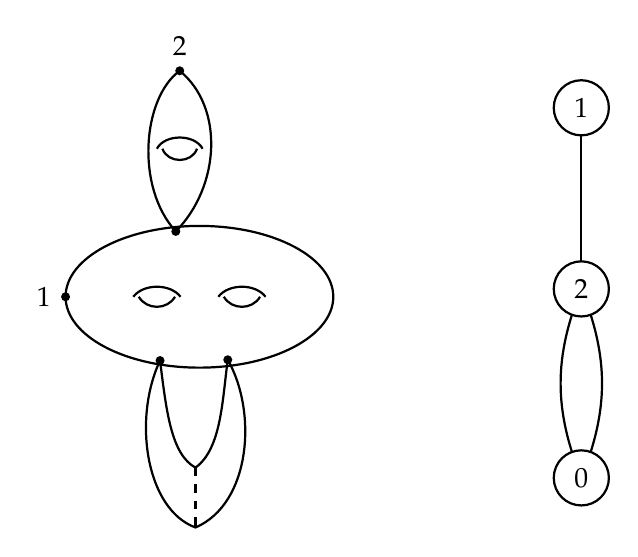
\begin{tikzpicture}[
        x=1cm,
        y=1cm,
        curve component/.style={thick},
        marked point/.style={circle,fill=black,inner sep=1.15pt},
        graph vertex/.style={
            circle,draw,thick,fill=white,minimum size=7mm,inner sep=0pt
        }
    ]
        % A three-component curve with components of genera 1, 2, and 0.
        \draw[curve component] (1.5,3.65) ellipse [x radius=1.7,y radius=0.9];

        % The two handles on the genus-two component.
        \draw[curve component]
            (0.66,3.65)
            .. controls (0.79,3.82) and (1.13,3.82) .. (1.26,3.65);
        \draw[curve component]
            (0.73,3.65)
            .. controls (0.83,3.48) and (1.09,3.48) .. (1.19,3.65);
        \draw[curve component]
            (1.74,3.65)
            .. controls (1.87,3.82) and (2.21,3.82) .. (2.34,3.65);
        \draw[curve component]
            (1.81,3.65)
            .. controls (1.91,3.48) and (2.17,3.48) .. (2.27,3.65);

        % The genus-one component attached above.
        \coordinate (uppernode) at (1.2,4.48);
        \draw[curve component]
            (uppernode)
            .. controls (0.68,5.05) and (0.78,6.18) .. (1.25,6.52)
            .. controls (1.82,6.05) and (1.76,5.05) .. cycle;
        \draw[curve component]
            (0.96,5.53)
            .. controls (1.06,5.72) and (1.44,5.72) .. (1.54,5.53);
        \draw[curve component]
            (1.03,5.53)
            .. controls (1.10,5.34) and (1.40,5.34) .. (1.47,5.53);

        % The rational component attached at two nodes below.
        \coordinate (lowerleft) at (1.00,2.84);
        \coordinate (lowerright) at (1.86,2.85);
        \draw[curve component]
            (lowerleft)
            .. controls (0.65,2.10) and (0.82,0.95) .. (1.45,0.72)
            .. controls (2.15,1.02) and (2.24,2.18) .. (lowerright);
        \draw[curve component]
            (lowerleft)
            .. controls (1.08,2.20) and (1.14,1.65) .. (1.45,1.48)
            .. controls (1.78,1.72) and (1.79,2.34) .. (lowerright);
        \draw[curve component,dashed] (1.45,1.48) -- (1.45,0.72);

        % Nodes and marked points.
        \node[marked point] at (uppernode) {};
        \node[marked point] at (lowerleft) {};
        \node[marked point] at (lowerright) {};
        \node[marked point,label=left:{$1$}] at (-0.2,3.65) {};
        \node[marked point,label=above:{$2$}] at (1.25,6.52) {};

        % The dual graph: the vertex labels record the genera.
        \coordinate (vone) at (6.35,6.05);
        \coordinate (vtwo) at (6.35,3.75);
        \coordinate (vzero) at (6.35,1.35);
        \draw[curve component] (vone) -- (vtwo);
        \draw[curve component]
            (vtwo) to[out=-112,in=112] (vzero);
        \draw[curve component]
            (vtwo) to[out=-68,in=68] (vzero);
        \node[graph vertex] at (vone) {$1$};
        \node[graph vertex] at (vtwo) {$2$};
        \node[graph vertex] at (vzero) {$0$};
    \end{tikzpicture}
    \end{center}
\end{exm}

对对数或穿孔 R-映射
\begin{equation*}
\begin{tikzcd}
    & \mf{P} \ar{d} \\
    C \ar{ur}{f} \ar{d} \ar{r} & B \C_{\omega}^{\times} \\
    S,
\end{tikzcd}
\end{equation*}
我们通过取整个图表的相伴广义锥复形来进行热带化。由于 \(B \C_{\omega}^{\times}\) 没有对数结构，我们看到的是
\begin{equation*}
\begin{tikzcd}
    \Sigma(C) \ar{d} \ar{r}{\Sigma(f)} & \Sigma(\mf{P}) = \R_{\geq 0} \\
    \Sigma(S).
\end{tikzcd}
\end{equation*}
现在设 \(S = \Spec (Q \to \C)\) 为对数点，其中 \(Q\) 是 fs 尖幺半群。特别地，这意味着 \(\Sigma(S) = Q_{\R}^{\vee}\)。由于一切都是（分片）线性的，只需取一个内点 \(t \in \Sigma(S)\) 并考虑 \(\Sigma(C)_t\)。

对每条半边，我们把它视为从所连顶点指向外，特别地，这意味着到 \(\R_{\geq 0}\) 的线性映射对应一个斜率。我们称之为\textit{接触阶}。特别地，若 \(h \neq \hat{h}\) 由 \(\imath\) 相互关联，则 \(c(h) = - c(\hat{h})\)。对所有 \(v \in \V\)，我们还定义\textit{退化度}
\[ e_v \colon Q_{\R}^{\vee} \to \R_{\geq 0} \qquad t \mapsto \Sigma(f)_t (v). \]
特别地，\(e_v \in Q\) 是一个整点。

接下来需要引入的是穿孔腿。它们记为
\[ \L^{\circ} = \ab\{ h \in \H \mid \Sigma(f)_t(h) \text{ is bounded and nontrivial for all } t \in Q_{\R}^{\vee}\}. \] 
我们对满足 \(0 \in \ol{\Sigma(f)_t(h)}\) 的 \(h \in \L^{\circ}\) 定义预稳定性，这是一个技术上必要的假设。在所有穿孔腿都预稳定的假设下，我们可以定义\textit{边长}函数
\[ \ell \colon \E \cup \L^{\circ} \to \ms{Map}(Q_{\R}^{\vee}, \R_{\geq 0}) \qquad x \mapsto \ell(x) \colon t \mapsto \ell(x)(t). \]
注意对边 \(E\) 而言 \(\ell(E) \in Q\) 也是一个整点。对穿孔腿，这一结论在相差一个细分的意义下成立。


\subsection{对数 GLSM 不变量}%
\label{sub:Log GLSM invariants}

\begin{defn}
    我们将对数映射 \(f\) 的\textit{装饰热带型}（decorated tropical type）定义为
    \[ \bm{\tau} = (G, c \colon \H \to \Z, \beta \colon \V \to H_2(X)). \]
\end{defn}

\begin{defn}
    一个对数映射或穿孔映射 \(f\) 称为\textit{紧致型}（compact type）的，如果
    \begin{enumerate}
        \item \(\Ima \Sigma(f)_t\) 对所有 \(t\) 都有界；
        \item 对所有接触阶为 \(0\) 的半边 \(h\) 有 \(f(p_h) \in 0_{\mf{P}}\)。
    \end{enumerate}
\end{defn}

现在我们可以定义范畴 \(\mc{R}(\mf{P}, \tau)\)，它由纤维在 fs 对数概形范畴 \(\ms{LogSch}\) 之上、以 \(\tau\) 标记的稳定穿孔 R-映射组成。

\begin{thm}[{\cite{CJR2021,CJRpunctured}}]
    叠 \(\mc{R}(\mf{P},\bm{\tau})\) 由一个带基本/最小对数结构的真 DM叠代表。
\end{thm}

\begin{rmk}
    若 \(\V = \ab\{v\}\) 为单点集，则我们记
    \[ \mc{R}_{g, c}(\mf{P}, \beta) \coloneqq \mc{R}(\mf{P}, \bm{\tau}). \]
\end{rmk}

考虑下图
\begin{equation*}
\begin{tikzcd}
    & \mf{P} \ar{d} \\
    \mc{C} \ar{ur}{f} \ar{d}{\pi} \ar{r} & B \C_{\omega}^{\times} \\
    \mc{R},
\end{tikzcd}
\end{equation*}
其中我们置 \(\mc{R} \coloneqq \mc{R}(\mf{P}, \bm{\tau})\)。于是完美障碍理论由
\[ T_{\mc{R}/\ms{Log}_{\mf{M}_G}} \to \E_{\square} = R \pi_* f^* T_{\mf{P}/B\C_{\omega}^{\times}}. \]
定义。这里两个切丛均指对数切复形。由完美障碍理论，这定义了典范虚类
\[ [\mc{R}(\mf{P}, \bm{\tau})]^{\vir}. \]
这个虚类的主要缺点是它不能重现 Gromov–Witten 理论。不过，我们可以考察它与 GW 理论的差别，但这需要一个双有理修正。设 \(Q\) 为尖幺半群。它有一个偏序：\(a < b\) 是指存在非零 \(c \in Q\) 使得 \(a+c = b\)。

\begin{defn}
    我们称 \(f\) 或 \(\Sigma(f)\) 具有\textit{一致极大退化}（uniform maximal degeneracy），如果存在 \(e_{\max} \in \ab\{e_v \mid v \in \V \}\) 使得对所有 \(v \in \V\) 有 \(e_{\max} \geq e_v\)。
\end{defn}

\begin{rmk}
    若 \(f\) 为紧致型且具有一致极大退化，则 \(\Sigma(f)\) 被 \(e_{\max}\) 一致有界。
\end{rmk}

\begin{defn}
    定义 \(\mc{U}(\mf{P}, \bm{\tau})\) 为以 \(\bm{\tau}\) 标记且具有一致极大退化的稳定穿孔或对数 R-映射的叠。
\end{defn}

\begin{rmk}
    若 \(\V = \ab\{v\}\) 为单点集，则我们记
    \[ \mc{U}_{g, c}(\mf{P}, \beta) \coloneqq \mc{U}(\mf{P}, \bm{\tau}). \]
    若某个接触阶为负，则我们记
    \[ \mc{U}_{g, c}(\infty, \beta) \coloneqq \mc{U}(\mf{P}, \bm{\tau}). \]
\end{rmk}

注意到顶点分为两类：若顶点映到 \(0\)，则或者至少有一条半边向上指，或者所有接触阶均为 \(0\)，此时全部收缩。这些称为\textit{对数顶点}（log vertex）。另一类顶点是不映到 \(0\) 的顶点：或者所有半边都向下指，或者有一些半边向上指。这些称为\textit{\(\infty\)-顶点}。此外，紧致型的顶点即那些没有向上指半边的顶点。

若忘掉一致极大退化这一条件，则有一个态射
\[ \mc{U}(\mf{P}, \bm{\tau}) \xrightarrow{F} \mc{R}(\mf{P}, \bm{\tau}) \]
它是 \(\ms{LogSch}\) 上的子范畴。然而，作为代数叠之间的态射，它是对数 étale、真且满射的。此外，\(\mc{U}\) 具有由 \(\mc{R}\) 拉回的典范完美障碍理论。当顶点集为单点集时，我们有
\begin{align*}
    F_* [\mc{U}_{g, c}(\mf{P}, \beta)]^{\vir} &= [\mc{R}_{g, c}(\mf{P}, \beta)]^{\vir}; \\
    F_* [\mc{U}_{g, c}(\infty, \beta)]^{\vir} &= [\mc{R}_{g, c}(\infty, \beta)]^{\vir}.
\end{align*}
在对数顶点的情形，我们实际上有从带 p-场的稳定映射模空间出发的包含
\begin{equation*}
\begin{tikzcd}
    \mc{U} \ar{rr}{F} & & \mc{R} \\
    & \mc{R}_{g,c}(\mf{P}^{\circ}, \beta) \ar[hookrightarrow]{ul} \ar[hookrightarrow]{ur}.
\end{tikzcd}
\end{equation*}
若记 p-场的模空间为 \(\mc{R}^{\circ}\)，则边界
\[ \Delta \coloneqq \mc{U} \setminus \mc{R}^{\circ} \]
是一个 Cartier 除子。由一致极大退化的条件，我们有一个截面
\[ e_{\max} \in H^0(\bar{M}_{\mc{U}}). \]
这等价于一个态射
\[ \mc{U} \to ([\A^1/\G_m], 0) \]
的数据，它将 \(0\) 拉回为 \(\Delta\)。

我们将\textit{超势}（superpotential）定义为一个函数
\begin{equation*}
\begin{tikzcd}
    \mf{P}^{\circ} \ar{rr}{W} \ar{dr} && \mc{L}_{\omega} \ar{dl} \\
    & B \C_{\omega}^{\times}.
\end{tikzcd}
\end{equation*}
其\textit{临界轨迹}（critical locus）记为
\[ \on{Crit}(W) = (\d{W} = 0). \]
我们称 \(W\) 具有\textit{真临界轨迹}，若 \(\on{Crit}(W) \to B\C_{\omega}^{\times}\) 是真（proper）的。

例如，假设我们对 GW 理论感兴趣。设 \(X\) 为光滑射影簇，\(V\) 为 \(X\) 上的向量丛，\(s \in H^0(V)\)。令 \(Z = (s = 0)\)。于是我们得到
\[ W \colon \mf{P}^{\circ} = V^{\vee} \boxtimes \mc{L}_{\omega} \xrightarrow{s \otimes 1_{\omega}} \mc{L}_{\omega}. \]

\begin{lem}
    \(W\) 具有真临界轨迹当且仅当 \(Z\) 光滑且余维数为预期值。
\end{lem}

\begin{exm}
    设 \(X\) 为一点，\(V = \C\)，且 \(s \neq 0\)。则 \(\d{W} = s \neq 0\)，故临界轨迹为空。
\end{exm}

利用 Kiem–Li 的余截面局部化方法~\cite{KiemLi2013}，我们可以得到一个虚类
\[ [\mc{R}_{g, c=n}(\mf{P}^{\circ}, \beta)]_W^{\vir}, \]
它支撑在临界轨迹上。在 GW 理论中，它等于 GW 虚类
\[ \pm [\bar{M}_{g,n}(\on{Crit}(W), \beta)]^{\vir}, \]
其中符号可以显式算出。

\begin{thm}[{\cite{CJR2021,CJW2021}}]
    设 \(\bm{\tau}\) 为紧致型。在紧致型情形下，
    \begin{enumerate}
        \item \(\mc{U}(\mf{P}, \bm{\tau})\) 具有约化完美障碍理论，由此得到约化虚类 \([\mc{U}(\mf{P}, \bm{\tau})]^{\vir}\)；
        \item \(\Delta\) 具有约化完美障碍理论，由此得到约化虚类 \([\Delta]^{\vir}\)；
        \item 在单个对数顶点的情形，我们有 \([\mc{U}_{g, c=n}(\mf{P}, \beta)]^{\on{red}} = \pm [\bar{M}_{g,n}(\on{Crit}(W), \beta)]^{\vir}\)。此外还有公式
            \[ [\mc{U}_{g, c=n}(\mf{P}, \beta)]^{\on{red}} = [\mc{U}_{g, c=n}(\mf{P}, \beta)]^{\vir} - \tilde{r} [\Delta]^{\on{red}}, \]
            其中 \(\tilde{r}\) 是 \(W\) 沿 \(\infty\) 的极点阶。
    \end{enumerate}
\end{thm}

\subsection{热带分解与有限生成}%
\label{sub:Tropical decomposition and finite generation}

下文的热带分解及其应用取自工作文稿~\cite{CJRtropical2025}。有效不变量及其公理在~\cite{CJRpunctured} 中发展。

从现在起，我们考虑一个更简单的设定：\(X\) 是光滑射影簇而 \(V\) 是 \(X\) 上的线丛。此时我们假设 \(Z = (s = 0)\) 是余维 \(1\) 的光滑子簇。进一步假设 \(Z\) 是 Calabi–Yau 三维簇。我们考虑不变量
\[ N_{g, \beta} \coloneqq \int_{[\bar{M}_{g,0}(Z, \beta)]^{\vir}} 1 \in \Q \]
与生成级数
\[ F_g = \sum_{\beta \geq 0} N_{g, \beta} Q^{\beta} \in \Lambda \coloneqq \C \ps{Q}. \]

\begin{conj}[Yamaguchi-Yau, Alim-L\"ange {\cite{YY2004,AlimLange2007}}]
    假设 \(Z\) 满足 \(g=0\) 镜像对称。则存在有限生成的 \(\Q\)-代数 \(R \subset \Lambda\)，使得对所有 \(g \geq 2\) 有 \(F_g \in (I_0(q))^{2g-2} R\)。
\end{conj}

我们的主要目标如下。

\begin{thm}[{\cite{CJRtropical2025}}]
    设 \(Z\) 是 Fano 四维簇 \(X\) 中的 Calabi–Yau 三维超曲面，且 \(X\) 无奇上同调。设 \(\{\phi_j\}\) 是 \(H^*(X)\) 的一组基，\(\ab\{\phi^j\}\) 为对偶基。则对所有 \(g \geq 0\)，我们有
    \begin{align*}
        &F_g = (-1)^{1-g} \sum_{\tau' \in G_g'} \frac{(-1)^{\abs{\V_{\infty}}}}{\abs{\Aut(\tau')}} \cdot \prod_{E \in \E} c(E) \\
        & \cdot \sum_{j_E \mid E = \ab\{E_{\log}, E_{\infty}\} \in \E} \prod_{\substack{v \in \V_{\infty} \\ g(v)=1 \\ \H_v = \ab\{E_{\infty}\}}} c_1^{\mr{eff}}(\phi^{j_E}) \cdot \prod_{\substack{v \in \V_{\infty} \\ g(v) \geq 2}} \tilde{Q}^{\beta(v)} \cdot \exp \ab(\int_{\beta(v)} K(Q) )  \\
        & \cdot \ab(\prod_{E_{\infty} \in \H_v'}\int_{\beta(v)} \phi^{j_E}) \cdot c_{g(v), \beta(v)}^{\on{eff}} 
         \cdot \prod_{v \in \V_{\log}} \Omega_{g(v), \abs{\H_1(v)}, \abs{\H_2(v)}} (\phi_{j_E} \colon E_{\log} \in \H_1(v)).
    \end{align*}
\end{thm}

\begin{exm}
    设 \(Y\) 为带其环面对数结构的环面簇。则 \(\Sigma(Y)\) 是视为锥复形的环面扇，我们可以考虑其边界 \(\Delta_Y = \sum_{\rho \in \Sigma(Y)^1} \Delta_{\rho}\)。
\end{exm}

若我们考虑 \([\Delta]^{\on{red}}\)，应当得到类似的公式
\[ [\Delta]^{\on{red}} = \sum_{\rho \in \Sigma(\Delta)(1)} [\Delta_{\rho}]^{\on{red}}. \]
现在的问题是 \(\rho\) 代表什么。事实上，它们参数化刚性热带曲线。在热带化
\begin{equation*}
\begin{tikzcd}
    \Sigma(C)_{\rho} \ar{d} \ar{r} & \Sigma(\mc{C}) \ar{r}{f} \ar{d} & \R_{\geq 0} \\
    \rho \ar[hookrightarrow]{r} & \Sigma(\mc{U}),
\end{tikzcd}
\end{equation*}
中，我们看到 \(f_{\rho}\) 是刚性的当且仅当源热带曲线是一个二部图，其中一组顶点映到 \(e_{\max}\) 而另一组顶点映到 \(0\)。

\begin{exm}
    设 \(X\) 为一点且 \(Z = \emptyset\)。再考虑 \(g = 2, n = 0\)。此时可能的图如~\Cref{fig:tropgraphs} 所示。
    \begin{figure}[htpb]
    \begin{center}
    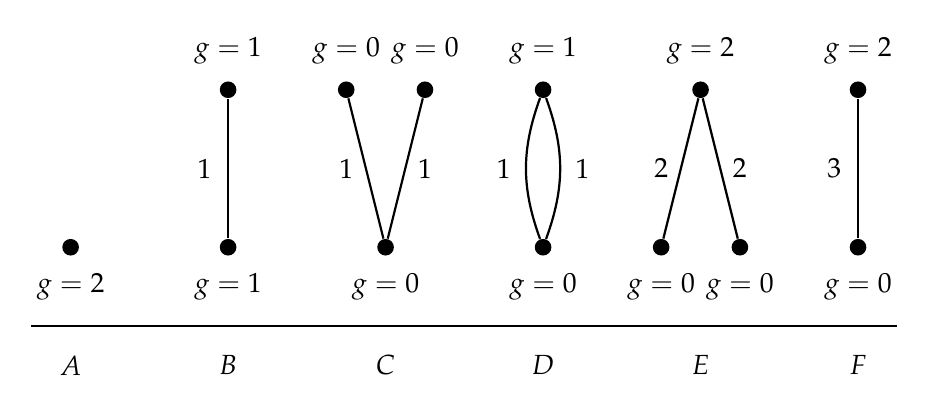
\begin{tikzpicture}[scale=1, transform shape]
        \node[fill=black,circle,minimum size=6pt,inner sep=0pt] (A) at (0,0) {};
        \node[fill=black,circle,minimum size=6pt,inner sep=0pt] (B1) at (2,0) {};
        \node[fill=black,circle,minimum size=6pt,inner sep=0pt] (B2) at (2,2) {};
        \node[fill=black,circle,minimum size=6pt,inner sep=0pt] (C1) at (4,0) {};
        \node[fill=black,circle,minimum size=6pt,inner sep=0pt] (C2) at (3.5,2) {};
        \node[fill=black,circle,minimum size=6pt,inner sep=0pt] (C3) at (4.5,2) {};
        \node[fill=black,circle,minimum size=6pt,inner sep=0pt] (D1) at (6,0) {};
        \node[fill=black,circle,minimum size=6pt,inner sep=0pt] (D2) at (6,2) {};
        \node[fill=black,circle,minimum size=6pt,inner sep=0pt] (E1) at (8,2) {};
        \node[fill=black,circle,minimum size=6pt,inner sep=0pt] (E2) at (7.5,0) {};
        \node[fill=black,circle,minimum size=6pt,inner sep=0pt] (E3) at (8.5,0) {};
        \node[fill=black,circle,minimum size=6pt,inner sep=0pt] (F1) at (10,0) {};
        \node[fill=black,circle,minimum size=6pt,inner sep=0pt] (F2) at (10,2) {};
        \draw[-,thick] (B1) -- (B2);
        \draw[-,thick] (C2) -- (C1) -- (C3);
        \draw[-,thick] (D1) edge[bend left=20] (D2);
        \draw[-,thick] (D2) edge[bend left=20] (D1);
        \draw[-,thick] (E2) -- (E1) -- (E3);
        \draw[-,thick] (F1) -- (F2);
        \node at (0,-0.5) {$g=2$};
        \node at (2,-0.5) {$g=1$};
        \node at (4,-0.5) {$g=0$};
        \node at (6,-0.5) {$g=0$};
        \node at (7.5,-0.5) {$g=0$};
        \node at (8.5,-0.5) {$g=0$};
        \node at (10,-0.5) {$g=0$};
        \node at (2,2.5) {$g=1$};
        \node at (3.5,2.5) {$g=0$};
        \node at (4.5,2.5) {$g=0$};
        \node at (6,2.5) {$g=1$};
        \node at (8,2.5) {$g=2$};
        \node at (10,2.5) {$g=2$};
        \draw[-,thick] (-0.5,-1) -- (10.5,-1);
        \node at (0,-1.5) {$A$};
        \node at (2,-1.5) {$B$};
        \node at (4,-1.5) {$C$};
        \node at (6,-1.5) {$D$};
        \node at (8,-1.5) {$E$};
        \node at (10,-1.5) {$F$};
        \node at (1.7,1) {$1$};
        \node at (3.5,1) {$1$};
        \node at (4.5,1) {$1$};
        \node at (5.5,1) {$1$};
        \node at (6.5,1) {$1$};
        \node at (7.5,1) {$2$};
        \node at (8.5,1) {$2$};
        \node at (9.7,1) {$3$};
    \end{tikzpicture}
    \end{center}
        \caption{当 $g=2$ 时 $X = \mr{pt}$、\(Z = \emptyset\) 的热带型的图。}%
    \label{fig:tropgraphs}
    \end{figure}
\end{exm}

\begin{thm}[热带量子莱夫谢茨 {\cite{CJRtropical2025}}]
    设 \(X\) 与 \(Z\) 同前。对任意 \(\beta \in H_2(X)\)、\(\alpha_1, \ldots, \alpha_n \in H^*(X)\) 以及 \(k_1, \ldots, k_n \in \N\)，我们有
    \begin{align*}
        \int_{[\bar{M}_{g,n}(Z,\beta)]^{\vir}} \prod_{j=1}^n \ev_j^* (\alpha_j) \psi^{k_j}={}& (-1)^{1-g+\beta \cdot Z} \cdot \sum_{\tau \vdash (g,n,\beta)} \frac{(-1)^{\abs{\V_{\infty}}}}{\abs{\Aut(\tau)}} \cdot \prod_{E \in \E} c(E) \\
        & \cdot \sum_{\ab\{j_E \mid E = \ab\{E_{\log}, E_{\infty}\}\}}  \prod_{v \in \V_{\infty}} \int_{[\mc{U}_v]^{\on{red}}} \prod_{E_{\infty} \in \H_v} \ev_{E_{\infty}}^* \phi^{j_E}  \\
        &  \cdot \prod_{v \in \V_{\log}} \int_{[\mc{R}_v]^{\vir}} \prod_{E_{\log}} \ev_{E_{\log}}^* (\phi_{j_E}) \cdot \prod_{h \in \L_v} \ev_h^* \alpha_h \cdot \psi_h^{k_h} .
    \end{align*}
\end{thm}

\begin{rmk}
    还有一个虚局部化公式，已在~\cite{CJRlocalization} 中宣布，它既可应用于约化理论（仅有 R-环面作用），也可应用于典范理论（可应用于环境空间的全部自同构）。
\end{rmk}

现在考虑一个 \(\infty\)-顶点。令 \(\tau_v = (g, c, \beta)\)，并令 \(\mc{U}_v = \mc{U}_{g,c}(\infty, \beta)\)。第一个计算是
\begin{align*}
    \on{red}\dim \mc{U}_v &= \chi(f^* T_{\mf{P}/B \C^{\times}_{\omega}}) + 1 + \on{trop}\dim  \\
    &= \vir\dim \bar{M}_{g,n}(Z, \beta) + \sum_{h \in \H } (c(h) + 1),
\end{align*}
其中热带维数为 \(3g-4+n\)。注意到所有接触阶都是负的，故第二项至多为零。特别地，我们已经证明了
\begin{cor}[{\cite{CJRpunctured}}]
    若 \(\vir\dim \bar{M}_{g,n}(Z,\beta) < 0\)，则 \([\mc{U}_v]^{\on{red}} = 0\)。
\end{cor}
我们还有一个\textit{平衡条件}（balancing condition），它断言
\begin{equation}\label{eqn:balancing condition}
    \sum_{h \in \H} c(h) = \deg f^* \mc{O}(\infty) = \int_{\beta} c_1(V) - (2g-2+n).
\end{equation}
这可以改写为
\[ 0 \geq \sum_{h \in \H} (c(h)+1) = \int_{\beta} c_1(V) - (2g-2). \]
\begin{prop}[{\cite{CJRpunctured}}]
    我们看到在下列情形下 \(\infty\)-顶点不存在：
    \begin{enumerate}
        \item \(g = 0\) 且 \(V\) 为 nef；
        \item \(g=1\) 且 \(V\) 为丰富，除非 \(\beta = 0\) 且所有 \(c(h) = -1\)。
    \end{enumerate}
\end{prop}

\begin{defn}
    一个标记称为\textit{单位}（unit），若其接触阶为 \(-1\)。
\end{defn}

\begin{notn}
    我们以 \(\1\) 记单位扇区，并记 \(\tau_{v+\1} = (g, c+\1, \beta)\)、\(\mc{U}_{v+\1} = \mc{U}_{g, c+\1}(\infty, \beta)\) 以及 \(\mc{R}_{v+\1} = \mc{R}_{g, c+\1}(\infty, \beta)\)。
\end{notn}

\begin{thm}[{\cite[Theorems~1.16--1.17]{CJRpunctured}}]\leavevmode
    \begin{enumerate}
        \item 存在态射 \(F_{\1} \colon \mc{U}_{v+\1} \xrightarrow{s} \mc{C}^{\circ} \xrightarrow{\pi} \mc{U}_v\)，其中 \(s\) 是双有理的；
        \item 约化虚类满足等式 \(s_* [\mc{U}_{v+\1}]^{\on{red}} = \pi^* [\mc{U}_v]^{\on{red}}\)；
        \item 若 \(D\) 是 \(X\) 上的除子，则 \(F_{\1 *} (\ev_{\1}^* D \cap [\mc{U}_{v+\1}]^{\on{red}}) = \ab(\int_{\beta} D) [\mc{U}_v]^{\on{red}}\)；
        \item 考虑下图
            \begin{equation*}
            \begin{tikzcd}
                \mc{U}_{v+\1} \ar{r}{F} \ar{d}[swap]{F_{\1}} & \bar{M}_{g,n+1} \ar{d}[swap]{p} \\
                \mc{U}_v \ar{r}{F} & \bar{M}_{g,n}.
            \end{tikzcd}
            \end{equation*}
            则 \(F_* [\mc{U}_{v+\1}]^{\on{red}} = p^* F_* [\mc{U}_v]^{\on{red}}\)。
    \end{enumerate}
\end{thm}

\begin{exm}
    考虑 \(g = 1\) 且 \(Z_d \subset X = \P^N\) 为超曲面的设定。我们只需考虑 \(\beta = 0\) 且对所有 \(h \in \H\) 有 \(c(h) = -1\) 的情形。于是我们看到
    \[ \prod_h \ev_h^* \alpha_h \cdot [\mc{U}_{1,c}(\infty,\beta)]^{\mr{red}} = \ev_{h^{\star}}^* \ab(\prod_h \alpha_h) \cap [\mc{U}_{1,\1}(\infty,\beta)]^{\on{red}}. \]
\end{exm}

\begin{prop}[{\cite{CJRpunctured}}]
    我们实际上有
    \[ \mc{U}_{1,\1}(\infty, 0) \simeq \mc{R}_{1,\1}(\infty, 0) \]
    以及等式
    \[ [\mc{U}_{1,\1}(\infty, 0)]^{\on{red}} = c_{\dim X} \ab(\mc{H}^{\vee} \boxtimes T_{\mf{P}/B\C_{\omega}^{\times}} + \mc{O} - V). \]
\end{prop}

\begin{exm}
    现在考虑五次三维簇 \(Z_5 \subset \P^4\)。于是我们看到 \(\on{red}\dim \mc{U}_v = \sum_{h \in \H} (c(h)+2)\)。单位公理把我们归约到 \(c(h) \leq -2\) 的情形。现在我们必须确定当所有 \(c(h) = -2\) 时需要考虑的新不变量的个数，这等价于求可能的 \(\beta\) 的个数。平衡条件断言
    \begin{align*}
        \sum_{h \in \H} c(h) &= \int_{\beta} c_1(V) - (2g-2+n) \\
        &= 5\beta - (2g-2+n),
    \end{align*}
    由此可得 \(0 \geq \sum (c(h)+1) = 5\beta - (2g-2)\)，从而 \(\beta \leq \frac{2g-2}{5}\)。\footnote{这恰好是我们假设有限生成、全纯反常方程、轨形正则性以及 conifold 间隙条件时所预测的未知数个数。}
\end{exm}

\begin{conj}[Janda {\cite[Conjecture~1.6]{CJRtropical2025}}]\leavevmode
    \begin{enumerate}
        \item 我们有 \(K(Q) = \log I_0(q) \cdot c_1(K_X^{\vee}) - \frac{I_1}{I_0}\) \\
        \item 典范理论满足 \(\Omega \in I_0(q)^{2g-2+2n_1 + 3 n_2} \cdot R\)。
    \end{enumerate}
\end{conj}

\begin{cor}[{\cite[Theorem~1.7]{CJRtropical2025}}]
    关于 \((X, V)\) 的上述猜想蕴含 \(Z\) 的 Yamaguchi–Yau 有限生成。
\end{cor}


\section{五次三维簇高亏格 GW 不变量的结构（郭帅）}%
\label{sec:Structure of higher-genus GW invariants of the quintic (Shuai Guo)}

\subsection{问题}%
\label{sub:The problem (Guo)}

我们考虑五次三维簇 \(X = X_5 \subset \P^4\)，并问它包含多少条亏格 \(g\)、次数 \(d\) 的曲线。在亏格零时，答案从
\[ 2875, \qquad 609250, \qquad 317206375, \qquad \ldots \]
开始。

由于 \(X\) 是 Calabi–Yau 的，模空间 \(\Mbar_{g,n}(X,\beta)\) 的虚维数为零，且弦方程给出 \(\ab<\1, \gamma_2, \ldots, \gamma_n>_{g,n,\beta} = 0\)，除非 \((g,n,\beta) = (0,3,0)\)。因此我们如下定义初级不变量
\[ N_{g,\beta} \coloneqq \ab<>_{g,0,\beta} = \int_{[\Mbar_g(X,\beta)]^{\vir}} 1 \]
并把这些数组成生成级数
\[ F_g(Q) \coloneqq \sum_{\beta \text{ effective}} N_{g,\beta}Q^{\beta}. \]

不变量 \(N_{g,\beta}\) 是有理数，而我们真正想要的整数是 BPS 不变量 \(n_{g,\beta}\)。它们由正次数部分 \(F_g^+\) 通过多重覆盖变换定义
\[ \sum_{g \geq 0} F_g^+(Q)\lambda^{2g-2} = \sum_{\substack{g \geq 0 \\ \beta > 0}} n_{g,\beta} \sum_{k \geq 1} \frac{1}{k} \ab(2 \sin \frac{k\lambda}{2})^{2g-2}Q^{k\beta}. \]
注意，只有 \(n_{g,\beta}\) 被预期为整数，而且上面的那些数正是 \(n_{0,d}\)。

\begin{table}[htpb]
    \centering
    \caption{五次三维簇的主要 BPS 不变量 \(n_{g,d}\)}
    \label{tab:quinticbps}
    \begin{tabular}{crrrrr}
        \toprule
        \(g\) & \(d=1\) & \(d=2\) & \(d=3\) & \(d=4\) & \(d=5\) \\
        \midrule
        0 & 2875 & 609250 & 317206375 & 242467530000 & 229305888887625 \\
        1 & 0 & 0 & 609250 & 3721431625 & 12129909700200 \\
        2 & 0 & 0 & 0 & 534750 & 75478987900 \\
        3 & 0 & 0 & 0 & 8625 & \(-15663750\) \\
        4 & 0 & 0 & 0 & 0 & 49250 \\
        5 & 0 & 0 & 0 & 0 & 1100 \\
        6 & 0 & 0 & 0 & 0 & 10 \\
        7 & 0 & 0 & 0 & 0 & 0 \\
        \bottomrule
    \end{tabular}
\end{table}

我们看到 \Cref{tab:quinticbps} 的每一列最终都消失。这就是 Castelnuovo 界，对五次情形它断言当 \(g > \frac{d^2+5d+10}{10}\) 时 \(n_{g,d} = 0\)，由刘治宇与阮勇斌~\cite{LiuRuanCastelnuovo} 证明。表中各数的整性即 Gopakumar–Vafa 猜想，由 Ionel--Parker~\cite{IonelParker2018} 证明。

在亏格零时，Candelas-de la Ossa-Green-Parkes 利用镜像上的周期积分计算了 \(F_0\)，这一点我们在 \Cref{sub:Enumerative mirror symmetry in genus zero} 中讨论过。在高亏格时，Bershadsky-Cecotti-Ooguri-Vafa 给出了一个递归，由 \(h < g\) 的 \(F_h\) 产生 \(F_g\)，但相差有限多个未知常数。我们的目标是解释对数 GLSM 如何确定这一歧义。

\subsection{亏格零与 B 模型的多项式结构}%
\label{sub:Genus zero and the polynomial structure of the B-model}

回忆 \Cref{sub:Enumerative mirror symmetry in genus zero}：对五次情形我们考虑 \(I\)-函数
\[
    I(q,z) = z\sum_{d \geq 0} q^{H/z+d} \frac{\prod_{m=1}^{5d}(5H+mz)}{\prod_{m=1}^d (H+mz)^5} = I_0 z + I_1 H + I_2 \frac{H^2}{z} + I_3 \frac{H^3}{z^2},
\]
其各分量被 Picard–Fuchs 算子
\[ D^4 - 5q(5D+1)(5D+2)(5D+3)(5D+4), \qquad D = q \odv{}{q}. \]
零化。若记 \(J_k = I_k/I_0\)，并令 \(\frac{I_1}{I_0} = \log q + \tau(q)\)，使得 \(Q = e^{I_1/I_0} = qe^{\tau(q)} = q + O(q^2)\)，则亏格零镜像定理断言
\[ F_0(Q) = \frac{5}{2}\ab(J_1 J_2 - J_3). \]

就我们的目的而言，把五次公式置于一般镜像对称的图景中是有用的。设 \(\mc{X} = \ab\{(X,\omega)\}\) 是 Calabi–Yau 三维簇的族，其 Kähler 模空间为 \(\mc{M} \ni Q = e^{2\pi i \omega}\)，再设 \(\mc{X}^{\vee} = \ab\{(X^{\vee},J)\}\) 为镜像族，其复模空间为 \(\mc{M}^{\vee} \ni q\)。Picard–Fuchs 方程的解是 \(X^{\vee}\) 上的周期，它们拼成
\[ I(z) = zI_0\varphi_0 + I_1 + I_2 z^{-1} + I_3 z^{-2}, \]
它落在 \(z\varphi_0, \varphi_{\alpha}, \varphi^{\alpha}z^{-1}, \varphi^0 z^{-2}\) 的张成中。这里 \(I_1 = \sum_{\alpha} I_1^{\alpha}\varphi_{\alpha}\)，\(I_2 = \sum_{\alpha} I_{2,\alpha}\varphi^{\alpha}\)，\(I_3 = I_{3,0}\varphi^0\)，而镜像映射仍为 \(Q = e^{I_1/I_0} = qe^{\tau(q)}\)。

我们将用到五次情形复模直线上的三个特殊点：大复结构点 \(q=0\)、锥点（conifold point）\(q = 5^{-5}\)（此处某个周期消失），以及轨形（orbifold）（或 Landau–Ginzburg）点 \(q = \infty\)。镜像映射在 \(q=0\) 处有定义，其在该处的展开给出格罗莫夫–威滕不变量；而在高亏格时，我们将在另外两点处施加边界条件。

我们现在用三点函数重新表述镜像定理。取 \(\mc{M}^{\vee}\) 上的局部坐标 \(q_i\)，设 \(\ab\{\phi_i\}\) 是 A 侧相应的基，并定义
\[ C^A_{ijk}(Q) \coloneqq I_0^2 \ab<\phi_i, \phi_j, \phi_k>^X_{0,3}, \qquad C^B_{ijk}(q) \coloneqq \int_{X^{\vee}} \partial_i \partial_j \partial_k \Omega \wedge \Omega. \]

\begin{thm}[镜像定理 {\cite{Givental1998,LLY1997}}]
    我们有 \(C^A_{ijk}(Q(q)) = C^B_{ijk}(q)\)。此外 \(C^B_{ijk} \in \Delta^{-1}\Q[q]\)，故它是 \(\mc{M}^{\vee}\) 上整体定义的亚纯函数，仅沿判别式有极点。
\end{thm}

特别地，乘以 \(I_0\) 的适当幂次并施加镜像映射之后，亏格零的生成函数成为 \(q\) 的有理函数，仅沿判别式有极点。因此它由有限多个系数决定。

\begin{exm}
    对超平面基下的五次情形，
    \[ C_{111} = \frac{5}{1-5^5 q}. \]
\end{exm}

\begin{exm}
    对 \(X = X_{3,3} \subset \P^2 \times \P^2\)，Yukawa 耦合为
    \begin{align*}
        C_{111} &= \frac{3^4 q_1 (2+3^3q_1+3^3q_2)}{\Delta}, & C_{222} &= \frac{3^4 q_2(2+3^3q_1+3^3q_2)}{\Delta}, \\
        C_{112} &= \frac{(1-3^3q_1-3^3q_2)(1+2\cdot 3^3 q_1 - 3^3 q_2)}{\Delta}, \\
        C_{122} &= \frac{(1-3^3q_1-3^3q_2)(1-3^3q_1+2\cdot3^3q_2)}{\Delta},
    \end{align*}
    其中
    \[ \Delta = 1 - 3\cdot3^3(q_1+q_2) + 3\cdot3^6(q_1^2 - 7q_1q_2+q_2^2) - 3^9(q_1+q_2)^3. \]
\end{exm}

在高亏格时，我们预期存在正规化势 \(f^A_{g,i}\)，满足
\[ f^A_{g,i}(Q(q)) = f^B_{g,i}(q) \in \Delta^{-(2g-2+n)}\Q[q], \]
其中右端由图和计算。

\subsection{BCOV 费曼规则}%
\label{sub:The BCOV Feynman rule}

B 模型费曼规则与全纯反常方程源自~\cite{BCOV1994}。对五次情形，张怀良、郭帅与李骏在~\cite{CGL2021} 中证明了多项式性，并在~\cite{CGL2026} 中证明了费曼规则。

我们现在把 BCOV 递归作为费曼规则来讨论。它来自辛变换量子化的一个有限维模型，如 \Cref{sub:Operator formalism and geometric quantization} 所述。设 \(\mc{H} = \mc{H}^- \oplus \mc{H}^+ \subset \mc{H}_{\infty}\) 是辛的，且 \(d+1 = \dim \mc{H}^+ = \dim \mc{H}^-\)，并置
\[ R = \begin{pmatrix} A & B \\ C & D \end{pmatrix} \in \End \mc{H}, \qquad \mc{Q}(\mbf{x},\bp) = (\bp, D^{-1}\mbf{x}) - \frac{1}{2}(\bp, D^{-1}C\bp). \]
给定总势 \(F(\hbar, \mbf{x})\)，我们用高斯积分形式地定义变换后的势
\[ f(\hbar, \mbf{x}) \coloneqq (\wh{R}F)(\hbar,\mbf{x}) = \ln \int e^{\hbar^{-1}(\mc{Q}(\mbf{x},\bp') - \mbf{x}'\bp') + F(\hbar,\mbf{x}')}\d{\mbf{x}'}\d{\bp'}. \]
按稳定相展开给出一个图和。其中 \(D^{-1}C\) 提供每条边上的传播子，\(F\) 提供顶点。

对 Calabi–Yau 三维簇，传播子按指标个数分别写成 \(S^{\varphi\varphi}\)、\(S^{\varphi}\) 与 \(S\)，而顶点是正规化的 A 模型关联函数
\[ P^A_{g,n}(Q) = I_0^{2-2g}\ab<\phi_1, \ldots, \phi_n>^X_{g,n}. \]
注意，这些与后文将出现的、求解量子微分方程的算子 \(S_{\tau}(z)\) 毫无关系。

\begin{exm}
    对五次情形在亏格二且无标记时，费曼规则为
    \begin{align*}
        f_2^B ={}& P_2 + \frac{1}{2}S^{\varphi\varphi}P_{1,1}^2 + \frac{1}{2}S^{\varphi\varphi}P_{1,2} + (S^{\varphi\varphi})^2 P_{1,1} + \frac{1}{8}(S^{\varphi\varphi})^2 P_{0,4} \\
        &+ \frac{1}{8}(S^{\varphi\varphi})^3 + \frac{1}{12}(S^{\varphi\varphi})^3 + \frac{\chi}{24}S^{\varphi}P_{1,1} + \frac{1}{2}\frac{\chi}{24}S^{\varphi}S^{\varphi\varphi} \\
        &+ \frac{1}{2}\frac{\chi}{24}\ab(\frac{\chi}{24}-1)S,
    \end{align*}
    其中 \(\chi = \chi(X_5) = -200\)。这是传播子的一个三次多项式。
\end{exm}

我们可以如 \Cref{sub:R-matrix action} 那样把它解释为稳定图和。顶点 \(v\) 贡献低亏格关联函数 \(P_{g_v, \on{val}(v)}\)；内边把两个插入与一个传播子缩并；腿记录其余的插入。每个图以 \(\frac{1}{\ab|\Aut \Gamma|}\) 加权。同往常一样
\[ g(\Gamma) = h^1(\Gamma) + \sum_v g_v, \qquad 2g_v - 2 + \on{val}(v) > 0, \]
而 \(f_g^B\) 是亏格 \(g\) 的所有稳定图的贡献之和。

\subsection{全纯反常方程}%
\label{sub:The holomorphic anomaly equation}

我们现在把递归改写为微分方程。B 模型振幅 \(\mc{F}_g(z,\bar{z})\) 不是全纯的，当 \(g \geq 2\) 时其非全纯性由下式给出
\[ \partial_{\bar{i}} \mc{F}_g = \frac{1}{2}\bar{C}_{\bar{i}}^{jk}\ab( D_j D_k \mc{F}_{g-1} + \sum_{r=1}^{g-1} D_j \mc{F}_r D_k \mc{F}_{g-r} ). \]
这里 \(C_{ijk}\) 是 Yukawa 耦合，\(\bar{C}_{\bar{i}}^{jk}\) 由 \(\bar{C}_{\bar{i}\bar{j}\bar{k}}\) 用 Weil–Petersson 度量上升两个指标得到，\(D_j\) 是 Hodge 线丛相应幂次上的协变导数。右端的两项对应 \(\Mbar_g\) 的两个边界层，即一个非分离结点与一个分离结点。\(\frac{1}{2}\) 用于忘掉两支的顺序。

若选取局部 \(\bar{\partial}\)-原函数
\[ \partial_{\bar{i}}S^{jk} = \bar{C}_{\bar{i}}^{jk}, \qquad \partial_{\bar{i}}S^j = G_{i\bar{\ell}}S^{\ell j}, \qquad \partial_{\bar{i}}S = G_{i\bar{\ell}}S^{\ell}, \]
则模去一个全纯项后，反常方程成为多项式偏微分方程
\[ \pdv{\mc{F}_g}{S^{jk}} = \frac{1}{2}\ab( D_jD_k \mc{F}_{g-1} + \sum_{r=1}^{g-1} D_j \mc{F}_r D_k \mc{F}_{g-r} ). \]
这些传播子仅在相差全纯张量的意义下有定义，这一自由度正是全纯歧义的来源。

\begin{rmk}
    在我们将用于五次情形的单参数正规化变量下，上式写成
    \[ -\partial_0 P_g = \frac{1}{2}P_{g-1,2} + \frac{1}{2}\sum_{r=1}^{g-1}P_{r,1}P_{g-r,1}, \qquad -\partial_1 P_g = 0. \]
\end{rmk}

为理解图和为何满足该方程，注意在无标记的势中，非全纯生成元只出现在边因子中。因此沿传播子方向求导会挑出一条边并将其割断。两个半边成为所得低亏格顶点上的标记，由除子方程，协变导数正对应于这些标记。割开一个圈得到 \(P_{g-1,2}\)，割开一条分离边得到 \(P_{g_1,1}P_{g_2,1}\)。

\begin{rmk}
    为明确起见，这一蕴含只是单向的。BCOV 图规则蕴含反常方程，但反常方程本身并不确定图规则。为恢复同一个解，我们还需要传播子的约定、低亏格顶点数据以及边界条件。
\end{rmk}

若所有低亏格顶点都已知，则右端已知，于是我们可以对非全纯生成元积分，得到
\[ P_g = P_g^{\mr{particular}} + f_g(Y), \]
其中有限生成给出全纯歧义
\[ f_g(Y) = P_g|_{A = B_1 = B_2 = B_3 = 0} = \sum_{i=0}^{3g-3}a_{i,g}Y^i, \qquad Y = (1-5^5q)^{-1}. \]
我们看到反常方程在每个亏格留下 \(3g-2\) 个未知系数。

\begin{rmk}
    对五次情形，次数零数据连同轨形正则性消去了这些自由度中的 \(\ceil{\frac{3g-3}{5}}+1\) 个，而锥点缝隙（conifold gap）条件再给出 \(2g-2\) 个条件，于是剩下
    \[ 3g-2 - \ab(\ceil*{\frac{3g-3}{5}}+1) - (2g-2) = \floor*{\frac{2g-2}{5}} \]
    个参数，它们是真正新的有效不变量。这恰好是 \Cref{eqn:balancing condition} 所预言的 \(\infty\)-顶点未知数的个数，即满足 \(\beta \leq \frac{2g-2}{5}\) 的 \(\beta\) 的个数。
\end{rmk}

于是我们得到物理学家提出的如下猜想性算法：BCOV 费曼规则、Landau–Ginzburg 点处的轨形正则性（LG/CY 对应的一种形式，对五次情形这是郭帅、阮勇斌与 Janda 的进行中工作），以及锥点缝隙条件。此外我们还可以加上 Gopakumar–Vafa 整性与 Castelnuovo 界。

\subsection{四种理论}%
\label{sub:Four theories}

回忆 \Cref{sec:Log GLSM (Qile Chen)}：对数 GLSM 带有两个虚圈。约化圈恢复五次格罗莫夫–威滕理论，而典范等变圈容许一个单位根特殊化，它是半单的，因而可用 Givental–Teleman 计算。二部图和
\[ \Omega^{\mr{GW}}_{g,n} = \sum_{\Gamma \text{ bipartite}} \frac{1}{\ab|\Aut \Gamma|} \ab( \prod_{v \in V_{\infty}(\Gamma)} c^{\mr{eff}}_{g_v,\beta_v}) \Cont^{\mr{can}}_{\Gamma} \]
用后者表达前者，代价是在 \(\infty\)-顶点处引入有效不变量 \(c^{\mr{eff}}_{g,\beta}\)。用形式参数 \(\mbf{C} = \ab\{c_{g,\beta}\}\) 替代这些不变量，就得到 \textit{扩张 \(\mbf{C}\)-族}，其顶点数据由亚纯与 rubber 对数 GLSM 理论提供。

我们将考虑以下四种理论。
\begin{itemize}
    \item \textit{\(t\)-扭几何理论} 置 \(\lambda_i = 0\) 并保留辅助权重 \(t\)。它同时有稳定映射版本与稳定商版本，其中商版本给出下文亏格二的局部化公式。
    \item \textit{形式五次}（formal quintic），即形式 \(\lambda\)-扭理论，置 \(t = 0\) 并令 \(\lambda_i = \zeta_5^i \lambda\)。它是半单 CohFT，故具有通用且可计算的 \(R\)-矩阵。
    \item \textit{扩张 \(\mbf{C}\)-族} 在两者之间插值，同时带有形式顶点与亚纯顶点的二部图就生活在其中。
    \item \textit{五次格罗莫夫–威滕理论} 由置 \(\mbf{C} = \mbf{C}^{\mr{eff}}\) 再令 \(\lambda \to 0\) 得到，它正是我们想要计算的理论。
\end{itemize}

\begin{warn}
    在高亏格时，\(t\)-扭稳定商理论的 \(t^0\) 系数并不等于形式 \(\lambda\)-扭理论的 \(\lambda^0\) 系数。
\end{warn}

\subsection{形式五次}%
\label{sub:The formal quintic}

形式五次及其全纯反常方程在~\cite{LhoPandharipande2019} 中被研究；与扩张理论的比较则在~\cite{GJRstructure} 中展开。

设 \(E = \mc{O}_{\P^4}(5)\)，并设 \(\pi \colon \mc{C} \to \Mbar_{g,n}(\P^4,d)\) 为泛曲线。\(t\)-扭圈为
\[ e(R\pi_* f^* E \otimes [1]) \cap [\Mbar_{g,n}(\P^4,d)]^{\vir}, \]
其中 \([1]\) 的等变第一陈类为 \(t\)。若改为从完全 \((\C^{\times})^5\)-等变圈出发，形式五次是单位根特殊化
\[ [\Mbar_{g,n}(\P^4,d)]^{\vir,\lambda} \coloneqq \ab( e(R\pi_*f^*E \otimes [1]) \cap [\Mbar_{g,n}(\P^4,d)]^{\vir}_{(\C^{\times})^5})\Big|_{t=0, \; \lambda_i = \zeta_5^i \lambda}, \]
其中 \(\zeta_5 = e^{2\pi i/5}\)。关系 \(H^5 = \lambda^5\) 使量子积一般地成为半单的，同时把 \(\lambda\) 保留为参数。

态空间、单位与配对由
\[ \mc{H}_{\lambda} = \Q(\lambda)[H]/(H^5-\lambda^5), \quad \1 = 1, \quad (\gamma_1,\gamma_2)^{\lambda} = \int_{\P^4, (\C^{\times})^5} e(\mc{O}(5))\gamma_1\gamma_2 \Big|_{\lambda_i = \zeta_5^i\lambda}, \]
给出，而 CohFT 类为
\[ \Omega^{\lambda}_{g,n}(\gamma_1, \ldots, \gamma_n) = \sum_{d \geq 0} q^d \rho_* \ab( \prod_{i=1}^n \ev_i^*(\gamma_i) \cap [\Mbar_{g,n}(\P^4,d)]^{\vir,\lambda}), \]
其中 \(\rho\) 忘掉映射并稳定化定义域。若以 \(\tau(q)H\) 作平移，其中 \(\tau(q) = I^{\lambda}_1(q)/I^{\lambda}_0(q)\)，则平移后的理论 \(\Omega^{\lambda,\tau}\) 是半单的。把系数域扩张到 \(\Q(\zeta_5,\lambda)\) 之后，幂等基满足
\[ \omega^{\lambda}_{g,n}(e_{\alpha_1}, \ldots, e_{\alpha_n}) = \sum_{\alpha}\Delta_{\alpha}^{g-1}\prod_i \delta_{\alpha,\alpha_i}. \]
于是 \Cref{thm:teleman} 给出
\[ \Omega^{\lambda,\tau}_{g,n} = \sum_{\Gamma \in G_{g,n}} \frac{1}{\ab|\Aut\Gamma|}\iota_* \Cont_{\Gamma} \]
其中装饰如 \Cref{sub:R-matrix action}。携带 \(\gamma\) 的腿取 \(R^{-1}(\bar{\psi})\gamma\)，边取
\[ V_R(z_1,z_2) = \frac{\sum_{\alpha} e_{\alpha}\otimes e^{\alpha} - \sum_{\alpha} R^{-1}(z_1)e_{\alpha} \otimes R^{-1}(z_2)e^{\alpha}}{z_1+z_2}, \]
顶点则取拓扑场论 \(\omega\)，缺失的保单位部分通过 \(T(z) = z(\1 - R^{-1}(z)\1)\) 插入到被遗忘的标记处。

\begin{rmk}
    我们看到边因子没有极点。置 \(z_2 = -z_1\) 并以形式 \(R^{-1}(z) = R^*(-z)\) 使用辛条件，分子就消失。因此它可被 \(z_1+z_2\) 整除，\(V_R\) 是两个余切线变量的幂级数。\(z_1^p z_2^q\) 的系数是置于结点处并配以 \(\bar{\psi}_1^p \bar{\psi}_2^q\) 的类，把它与相邻的两个拓扑场论张量缩并就把两支粘合起来。
\end{rmk}

\subsection{如何计算 \(R\)-矩阵}%
\label{sub:How to compute the R-matrix (Guo)}

为计算 \(R\)-矩阵，我们从形式等变 \(I\)-函数开始
\[ I^{\lambda}(q,z) = z\sum_{d\geq0}q^d \frac{\prod_{m=1}^{5d}(5H+mz)}{\prod_{m=1}^d ((H+mz)^5 - \lambda^5)} = zI_0 + I_1^{\lambda}H + z^{-1}I_2^{\lambda}H^2 + \cdots. \]
到 \(H\) 为止的系数与 \(\lambda\) 无关，故 \(I_1^{\lambda} = I_1 - I_0 \log q\)，且镜像平移 \(\tau(q) = I_1^{\lambda}(q)/I_0(q)\) 不含对数。置
\[ D = q\odv{}{q}, \qquad Y = (1-5^5q)^{-1}, \qquad L = Y^{1/5} \]
并引入基
\[ \phi_k = I_{1,1}\cdots I_{k,k}H^k, \qquad \bar{\phi}_k = I_0 L^{-k-1}\phi_k, \]
其中对角 Birkhoff 因子由如下递归定义
\[ I_{p,0} = I_p, \qquad I_{p,r} = \frac{I_{p-1,r-1}}{I_{r-1,r-1}} + D \ab( \frac{I_{p,r-1}}{I_{r-1,r-1}}), \quad 1 \leq r \leq p, \]
于是特别地 \(I_{1,1} = 1+D\tau\)。幂等元与典范坐标由
\[ e_{\alpha} = \frac{1}{5}\sum_{i=0}^4 h_{\alpha}^{-i}\frac{\phi_i}{L^i}, \qquad u_{\alpha} = h_{\alpha}\int_0^q (L(s)-1)\frac{\d{s}}{s}, \qquad h_{\alpha} = \zeta_5^{\alpha}\lambda. \]
给出。

我们将用量子微分方程确定 \(R\)-矩阵对 \(q\) 的依赖。基本解满足
\[ zDS_{\tau}(z) + S_{\tau}(z)H = M_{\tau}S_{\tau}(z), \qquad M_{\tau} = \dot{\tau}\star, \quad \dot{\tau} \coloneqq (1+D\tau)H = I_{1,1}H, \]
而在正规化典范方向 \(\alpha\) 上，稳定相渐近给出
\[ (S_{\tau})_{i\bar{\alpha}}(z)C_{\alpha}(z)^{-1} = e^{u_{\alpha}/z}R_{i\bar{\alpha}}(z), \]
于是
\[ (zD+h_{\alpha}L)R_{i\bar{\alpha}} = \sum_j (M_{\tau})_i^j R_{j\bar{\alpha}}. \]
这里 \(C_{\alpha}(z)\) 是 \(q=0\) 处的量子 Riemann–Roch（等价地，Gamma 函数）因子，它与辛条件一起确定微分方程无法察觉的那些常数。与 \Cref{sub:How to compute the R-matrix} 末尾一样，微分方程给出递归，而振荡积分给出初始条件。

记 \(R(z) = \mr{Id} + R_1 z + R_2 z^2 + \cdots\)，我们就可以用上面的方程由前面各项逐个确定 \(R_{k+1}\)。有两个特点使五次情形可以处理。第一，单位根基有五个扇区，一条 mod \(5\) 的荷规则在每一行只允许一种剩余模式。于是大多数矩阵元在任何计算开始之前就已消失。第二，每个系数都落在有限生成环
\[ \mc{R} = \Q[A,B_1,B_2,B_3,Y], \qquad A = \frac{DI_{1,1}}{I_{1,1}}, \quad B_k = \frac{D^k I_0}{I_0}, \]
中，因此稳定图和归结为有限的代数计算。

\begin{rmk}
    特别地，由维数原因，固定的亏格只需要 \(R\) 的有限多项。在 \(\Mbar_{g,n}\) 上只有总次数至多 \(3g-3+n\) 的类有贡献，其余的都积分为零，故对无标记的势我们只需 \(R_0, \ldots, R_{3g-3}\)。亏格 \(4\) 到 \(z^9\) 为止，亏格 \(5\) 到 \(z^{12}\) 为止。
\end{rmk}


\subsection{亏格二}%
\label{sub:Genus two}

这里讨论的亏格二镜像公式出自郭帅、Janda 与阮勇斌~\cite{GJRgenus2}。

现在我们在亏格二中同时执行两条路线。几何路线使用 \(t\)-扭曲稳定商理论，先用虚拟局部化得到五项贡献，再用稳定商越墙（wall-crossing）过渡到五次格罗莫夫–威滕理论。形式路线则使用半单的 \(\lambda\)-扭曲理论和 \(R\)-矩阵来计算稳定图和。这只给出形式主部，之后还必须补上有效与亚纯的其余图（rest graphs）。

\begin{notn}
    记
    \[ \ab<\alpha_1, \ldots, \alpha_n>^{t,\mr{SQ}}_{g,n} \coloneqq \sum_{d\geq0}q^d \int_{[\Mbar_{g,n}(\P^4,d)]^{\vir}}e(R\pi_*\mc{L}^{\otimes 5}\otimes[-1])\prod_i \ev_i^*(\alpha_i), \]
    其中 \(\mc{L}\) 是泛稳定商线丛，且 \(c_1^{\C^{\times}}([-1]) = -t\)（这一符号约定下文还会再提到）。这是稳定商的符号约定，与上文稳定映射圈中出现的 \([1]\) 并不相同。
\end{notn}

\begin{figure}[htpb]
    \centering
    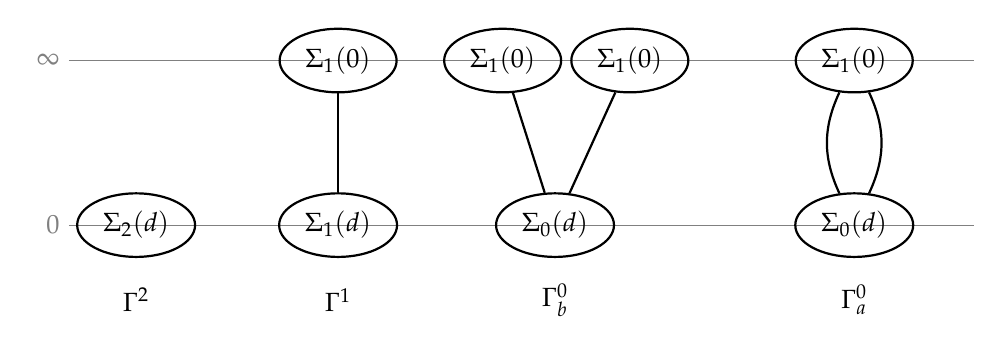
\begin{tikzpicture}[scale=0.95,transform shape]
        \draw[gray] (-0.9,0) -- (11.2,0);
        \draw[gray] (-0.9,2.2) -- (11.2,2.2);
        \node[anchor=east,gray] at (-0.9,0) {$0$};
        \node[anchor=east,gray] at (-0.9,2.2) {$\infty$};
        \node[ellipse,draw,thick,minimum width=1.5cm,minimum height=0.75cm] (a) at (0,0) {$\Sigma_2(d)$};
        \node at (0,-1) {$\Gamma^2$};
        \node[ellipse,draw,thick,minimum width=1.5cm,minimum height=0.75cm] (b0) at (2.7,0) {$\Sigma_1(d)$};
        \node[ellipse,draw,thick,minimum width=1.5cm,minimum height=0.75cm] (b1) at (2.7,2.2) {$\Sigma_1(0)$};
        \draw[thick] (b0) -- (b1);
        \node at (2.7,-1) {$\Gamma^1$};
        \node[ellipse,draw,thick,minimum width=1.5cm,minimum height=0.75cm] (c0) at (5.6,0) {$\Sigma_0(d)$};
        \node[ellipse,draw,thick,minimum width=1.5cm,minimum height=0.75cm] (c1) at (4.9,2.2) {$\Sigma_1(0)$};
        \node[ellipse,draw,thick,minimum width=1.5cm,minimum height=0.75cm] (c2) at (6.6,2.2) {$\Sigma_1(0)$};
        \draw[thick] (c0) -- (c1);
        \draw[thick] (c0) -- (c2);
        \node at (5.6,-1) {$\Gamma_b^0$};
        \node[ellipse,draw,thick,minimum width=1.5cm,minimum height=0.75cm] (d0) at (9.6,0) {$\Sigma_0(d)$};
        \node[ellipse,draw,thick,minimum width=1.5cm,minimum height=0.75cm] (d1) at (9.6,2.2) {$\Sigma_1(0)$};
        \draw[thick] (d0) to[bend left=25] (d1);
        \draw[thick] (d0) to[bend right=25] (d1);
        \node at (9.6,-1) {$\Gamma_a^0$};
    \end{tikzpicture}
    \caption{亏格二中四个非常值的局部化图，每个顶点画成其对应的黎曼面分支。}%
    \label{fig:g2loc}
\end{figure}

四个非常值图见~\Cref{fig:g2loc}，其贡献为
\begin{align*}
    \Cont_{\Gamma^2} &= \ab<>^{t,\mr{SQ}}_{2,0}, \\
    \Cont_{\Gamma^1} &= -\ab< \frac{-\frac{5}{2}H^3 + \frac{5}{24}H^4t^{-1}}{(t-5H)(t-5H-\psi)}>^{t,\mr{SQ}}_{1,1}, \\
    \Cont_{\Gamma_b^0} &= \ab< \frac{-\frac{5}{2}H^3+\frac{5}{24}H^4t^{-1}}{(t-5H)(t-5H-\psi_1)}, \frac{-\frac{5}{2}H^3+\frac{5}{24}H^4t^{-1}}{(t-5H)(t-5H-\psi_2)}>^{t,\mr{SQ}}_{0,2},
\end{align*}
对双边图记 \(H_1 = H \otimes 1\)、\(H_2 = 1 \otimes H\)，则
\[ \Cont_{\Gamma_a^0} = \ab< \frac{\frac{5}{3}(H^3\otimes H^4 + H^4 \otimes H^3)t^{-1} + \frac{65}{24}H^4 \otimes H^4 t^{-2}}{(t-5H_1)(t-5H_1-\psi_1)(t-5H_2)(t-5H_2-\psi_2)}>^{t,\mr{SQ}}_{0,2}. \]
注意到这些关联子是在 \(\P^4\) 上取的，故其中 \(H^4\) 出现且非零。

第五项贡献来自零次图，即常数
\[ -2c_{2,0} = -\frac{5}{144}, \qquad c_{2,0} = -\frac{1}{2}N_{2,0} = \frac{5}{288}, \]
把这五项贡献相加，我们得到局部化恒等式
\[ F_2^{\mr{SQ}}(q) = \Cont_{\Gamma^2} + \Cont_{\Gamma^1} + \frac{1}{2}\Cont_{\Gamma_a^0} + \frac{1}{2}\Cont_{\Gamma_b^0} - 2c_{2,0}, \]
其中两个 \(\frac{1}{2}\) 因子来自 \(\Gamma_a^0\) 与 \(\Gamma_b^0\) 的自同构。

设 \(Q = qe^{\tau(q)}\)、\(L = (1-5^5q)^{-1/5}\)，其中 \(\tau(q) = I_1(q)/I_0(q) - \log q\) 是通常的镜像平移。现在应用稳定商越墙，得到精确恒等式
\[ F_2^{\mr{GW}}(Q) = I_0(q)^2 F_2^{\mr{SQ}}(q). \]
引入 \(D_u = L^{-1}q\odv{}{q}\) 以及生成元
\[ \mc{X}_k = D_u^k \log \frac{I_0}{L}, \qquad \mc{Y}_k = D_u^k \log \frac{I_0I_{1,1}}{L^2}, \qquad I_{1,1} = 1 + q \odv{\tau}{q}, \quad D_u L = \frac{1}{5}(L^5-1), \]
各个扭曲图的贡献还涉及额外的生成元。对我们来说关键的一点是：这些生成元在上述线性组合中相互抵消，恰好留下有限生成变量。记 \(X = \mc{X}_1\)、\(Y_1 = \mc{Y}_1\)，我们得到
\begin{align*}
    F^{\mr{GW}}_2(Q) = \frac{I_0^2}{L^2}\Big(&\frac{70}{9}\mc{X}_3 + \frac{575}{18}X\mc{X}_2 + \frac{557}{72}X^3 + \frac{5}{6}Y_1\mc{X}_2 \\
    &- \frac{629}{72}Y_1X^2 - \frac{23}{24}Y_1^2 X - \frac{1}{24}Y_1^3 \\
    &+ \frac{125}{36}\mc{X}_2 L^4 - \frac{5}{24}X^2L^4 - \frac{35}{9}Y_1XL^4 - \frac{5}{24}Y_1^2L^4 \\
    &- \frac{1441}{300}XL^3 - \frac{41}{300}Y_1L^3 + \frac{31459}{7200}XL^8 + \frac{2141}{7200}Y_1L^8 \\
    &+ \frac{29621}{12000}L^{12} - \frac{116369}{36000}L^7 + \frac{547}{750}L^2\Big).
\end{align*}
在大半径处展开，我们得到
\[ F_2^{\mr{GW}}(Q) = -\frac{5}{144} + \frac{575}{48}Q + \frac{5125}{2}Q^2 + \frac{7930375}{6}Q^3 + O(Q^4), \]
这些系数是格罗莫夫–威滕不变量 \(N_{2,d}\)，而非~\Cref{tab:quinticbps} 中的 BPS 整数。

现在转向形式路线。\(\Omega^{\lambda}_{2,0}\) 的 Givental-Teleman 公式是对无腿的七个亏格二稳定图求和，这些图见~\Cref{fig:g2stable}。只需用到 \(R^{-1}(z)\) 直到 \(z^3\) 的部分，而平移把这七种拓扑展开成 \(17\) 个带装饰的层（strata）。

\begin{figure}[htpb]
    \centering
    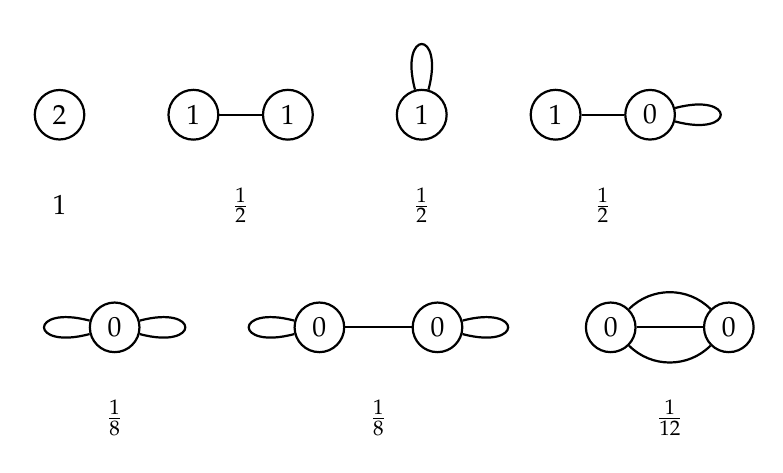
\begin{tikzpicture}[scale=1,transform shape,every loop/.style={min distance=8mm,looseness=10}]
        \node[circle,draw=black,thick] (a) at (0,0) {$2$};
        \node at (0,-1.15) {$1$};

        \node[circle,draw=black,thick] (b1) at (1.7,0) {$1$};
        \node[circle,draw=black,thick] (b2) at (2.9,0) {$1$};
        \draw[thick] (b1) -- (b2);
        \node at (2.3,-1.15) {$\frac{1}{2}$};

        \node[circle,draw=black,thick] (c) at (4.6,0) {$1$};
        \draw[thick] (c) edge[loop above] (c);
        \node at (4.6,-1.15) {$\frac{1}{2}$};

        \node[circle,draw=black,thick] (d1) at (6.3,0) {$1$};
        \node[circle,draw=black,thick] (d2) at (7.5,0) {$0$};
        \draw[thick] (d1) -- (d2);
        \draw[thick] (d2) edge[loop right] (d2);
        \node at (6.9,-1.15) {$\frac{1}{2}$};

        \node[circle,draw=black,thick] (e) at (0.7,-2.7) {$0$};
        \draw[thick] (e) edge[loop left] (e);
        \draw[thick] (e) edge[loop right] (e);
        \node at (0.7,-3.85) {$\frac{1}{8}$};

        \node[circle,draw=black,thick] (f1) at (3.3,-2.7) {$0$};
        \node[circle,draw=black,thick] (f2) at (4.8,-2.7) {$0$};
        \draw[thick] (f1) -- (f2);
        \draw[thick] (f1) edge[loop left] (f1);
        \draw[thick] (f2) edge[loop right] (f2);
        \node at (4.05,-3.85) {$\frac{1}{8}$};

        \node[circle,draw=black,thick] (g1) at (7.0,-2.7) {$0$};
        \node[circle,draw=black,thick] (g2) at (8.5,-2.7) {$0$};
        \draw[thick] (g1) -- (g2);
        \draw[thick] (g1) to[bend left=45] (g2);
        \draw[thick] (g1) to[bend right=45] (g2);
        \node at (7.75,-3.85) {$\frac{1}{12}$};
    \end{tikzpicture}
    \caption{无腿的七个亏格二稳定图，顶点处标以其亏格，并赋以权 \(\frac{1}{\ab|\Aut\Gamma|}\)。在幻灯片中每个顶点都画成其对应的黎曼面分支。}%
    \label{fig:g2stable}
\end{figure}

\begin{rmk}
    这些是稳定曲线的对偶图，并非~\Cref{fig:tropgraphs} 中的图；后者是把热带分解公式应用于对数 GLSM 的约化理论所得的刚性热带型。此处两列拓扑恰好重合，但顶点在两边的含义不同：这里的顶点是定义域曲线的一个分支，其上承载一个拓扑场论张量；那里的顶点则是二部热带曲线的一个层（level），承载对数或 \(\infty\)-顶点模问题。
\end{rmk}

对于形式路线，我们内蕴地定义规范化势为
\[ P_2^{\lambda} \coloneqq \frac{Y}{I_0^2}F_2^{\lambda}, \qquad Y = L^5. \]
完整的图和落在 \(\Q[L,\mc{X}_1,\mc{X}_2,\mc{X}_3,\mc{Y}_1]\) 中，且等于
\begin{align*}
    P_2^{\lambda} ={}& -\frac{1}{128}L^{12} - \frac{23}{960}L^8\mc{X}_1 - \frac{9}{640}L^8\mc{Y}_1 + \frac{109}{16000}L^7 \\
    &- \frac{3}{80}L^4\mc{X}_1^2 - \frac{19}{320}L^4\mc{X}_1\mc{Y}_1 - \frac{3}{80}L^4\mc{Y}_1^2 - \frac{1}{64}L^4\mc{X}_2 \\
    &+ \frac{19}{1920}L^3\mc{X}_1 - \frac{47}{48000}L^2 \\
    &- \frac{67}{1152}\mc{X}_1^3 - \frac{101}{1152}\mc{X}_1^2\mc{Y}_1 - \frac{5}{48}\mc{X}_1\mc{Y}_1^2 - \frac{1}{24}\mc{Y}_1^3 \\
    &- \frac{25}{288}\mc{X}_1\mc{X}_2 - \frac{1}{48}\mc{X}_2\mc{Y}_1 - \frac{19}{1152}\mc{X}_3.
\end{align*}
为明确起见，这是精确的形式 \(\lambda\)-扭曲答案，并不是 \(F_2^{\mr{GW}}\)。另请注意，\(Y = L^5\) 是判别式生成元，而 \(\mc{Y}_1\) 是对数导数生成元。

\subsection{有限生成与扩张族}%
\label{sub:Finite generation and the extended family}

回顾上文的有限生成环 \(\mc{R} = \Q[A,B_1,B_2,B_3,Y]\)，我们按下式分次
\[ \deg A = \deg B_1 = 1, \qquad \deg B_2 = 2, \qquad \deg B_3 = 3, \qquad \deg Y = 0. \]
对如前的 \(\phi_k = I_{1,1}\cdots I_{k,k}H^k\)，置
\[ \wt{\Omega}^{\lambda}_{g,n} \coloneqq 5^{g-1}\ab(\frac{Y}{I_0^2})^{g-1}\Omega^{\lambda,\tau}_{g,n}. \]

\begin{thm}[分次有限生成 {\cite{GJRstructure}}]%
\label{thm:graded finite generation}
    我们有
    \[ \wt{\Omega}^{\lambda}_{g,n}(\phi_{a_1}, \ldots, \phi_{a_n}) \in \bigoplus_{k \geq 0}\lambda^{5k}H^{2(3g-3+\sum_i a_i - 5k)}(\Mbar_{g,n},\Q)\otimes \mc{R}_{3g-3+\sum_i a_i}. \]
    于是，在拼装二部其余图之后，扩张族的非等变分量满足
    \[ P^{\mbf{C}}_{g,n} = 5^{1-g}\int_{\Mbar_{g,n}}\wt{\Omega}^{\mbf{C}}_{g,n}(\phi_1^{\otimes n}) = \ab( \frac{Y}{I_0^2})^{g-1}\int_{\Mbar_{g,n}}\Omega^{\mbf{C}}_{g,n}(\phi_1^{\otimes n}) \in \mc{R}_{3g-3+n}. \]
\end{thm}

特别地，对每个固定的 \((g,n)\)，只可能出现有限多个分次单项式，并且只有 \(R\)-矩阵直到 \(3g-3+n\) 阶的部分才有贡献。

我们用二部图和来组织扩张理论
\[ \Omega^{\mbf{C},\lambda}_{g,n} = \sum_{\Gamma \text{ bipartite}} \frac{1}{\ab|\Aut\Gamma|}\prod_{v\in V_{\infty}(\Gamma)} C^{\infty}_{g_v,\mu_v}(\mbf{C};\vec{a}_v) \prod_{v \in V_0(\Gamma)}C^{\lambda}_{g_v,\vec{\delta}_v}(\vec{a}_v)\prod_{e \in E(\Gamma)}V_e, \]
其中 \(C^{\infty}\) 是有效或亚纯的顶点因子，\(C^{\lambda}\) 是形式零顶点关联子，\(\mu_v\) 与 \(\vec{\delta}_v\) 记录关联次数，\(V_e\) 是边因子。极限 \(\lambda \to 0\) 只在完整的图和取完之后才取。置 \(\mbf{C}=0\) 只留下形式 \(\lambda\)-扭曲的主扇区。置 \(\mbf{C}=\mbf{C}^{\mr{eff}}\) 并令 \(\lambda\to0\) 则恢复五次格罗莫夫–威滕理论。对泛边求导会把它切断并产生全纯反常方程，同时保持有效顶点不变。

为导出全纯反常方程，记 \(P^{\mbf{C}}_g \coloneqq P^{\mbf{C}}_{g,0}\)，并引入
\[ \mc{U} = B_1, \qquad \mc{V} = A + 2B_1, \qquad \mc{V}_2 = D\mc{U} + \mc{U}^2 - \mc{U}\mc{V}, \qquad \mc{V}_3 = (D+\mc{V})\mc{V}_2, \]
以及两个非全纯方向
\[ \partial_1 = \partial_{\mc{U}}, \qquad \partial_0 = \partial_{\mc{V}} - \mc{U}\partial_{\mc{V}_2} - \mc{U}^2\partial_{\mc{V}_3}. \]

\begin{thm}[扩张族的全纯反常方程 {\cite{GJRstructure}}]
    我们有
    \[ -\partial_0 P^{\mbf{C}}_g = \frac{1}{2}P^{\mbf{C}}_{g-1,2} + \frac{1}{2}\sum_{\substack{g_1+g_2=g\\g_1,g_2\geq1}}P^{\mbf{C}}_{g_1,1}P^{\mbf{C}}_{g_2,1}, \qquad -\partial_1 P^{\mbf{C}}_g = 0. \]
\end{thm}

我们用~\Cref{sub:The holomorphic anomaly equation} 中的切割论证来证明它，该论证之所以可行，是因为 \(R\)-矩阵传播子的导数就是
\[ 5\mc{B}_{\partial_0} = \bar{\phi}_1 \otimes \bar{\phi}_1, \qquad 5\mc{B}_{\partial_1} = \bar{\phi}_0\otimes\bar{\phi}_2 + \bar{\phi}_2\otimes\bar{\phi}_0. \]
\(R^{-1}\) 与每条边的导数仍留在同一个分次环内，故切断一条求过导的边就闭合到 \(\mc{R}\) 中更低亏格的关联子上。若置 \(\mbf{C}=0\)，则对形式 \(\lambda\)-扭曲理论得到同样的方程。

\subsection{边界条件}%
\label{sub:Boundary conditions}

我们将从两个来源获得关于全纯歧义（holomorphic ambiguity）的条件。

第一，我们使用在轨形或 Landau--Ginzburg 点 \(q = \infty\)（等价地 \(L \to 0\)）处的正则性。对形式的或已拼装的扩张势 \(F_g^{\star}\)，置
\[ \mc{P}_g^{\mr{orb},\star} \coloneqq \ab(\frac{L}{I_0})^{2g-2}F_g^{\star} = \Phi_g^{\star}(\mc{X}_1,\mc{X}_2,\mc{X}_3,\mc{Y}_1,L^{-1},L^5). \]
\Cref{thm:graded finite generation} 给出了 \(L\) 的可能洛朗幂次的界，而形式的 LG/CY 等同断言：在解析延拓并把规范化 CY 基与 LG 基等同之后，同一个形式 \(R\)-矩阵多项式描述两个相。因此
\[ \lim_{L\to0}\Phi_g^{\star}(\mc{X}_1,\mc{X}_2,\mc{X}_3,\mc{Y}_1,L^{-1},L^5) \text{ exists}, \]
并且对 \(f_g(Y) = \sum_{i=0}^{3g-3}a_{i,g}Y^i\)（其中 \(Y = L^5\)），五次情形的界为
\[ a_{i,g} = 0 \qquad \text{for } i \leq \ceil*{\frac{3(g-1)}{5}}. \]
请注意，这是关于已拼装的规范化图贡献的论断，而不是关于单个的裸亚纯顶点或 rubber 顶点关联子。

第二，我们研究 conifold（锥奇点）。置
\[ q = 5^{-5}(1+t_c)^{-1}, \qquad T_c = \frac{I_1^{\mr{co}}(t_c)}{I_0^{\mr{co}}(t_c)}, \]
其中 \(I_0^{\mr{co}}, I_1^{\mr{co}}\) 构成局部的 conifold 周期对，规范化使得消没的平坦坐标在 conifold 处满足 \(T_c = 0\)。给定有限生成数据中的有理表达式 \(f\)，把所有生成元的洛朗展开代为 \(T_c\) 的幂级数，便得到它的 conifold 值 \(f^{\mr{co}}\)。\Cref{thm:graded finite generation} 给出极点界
\[ F_g^{\mbf{C},\mr{co}} = O\ab(T_c^{-(2g-2)}), \]
但我们需要的是更强的\textit{间隙}（gap）条件
\[ F_g^{\mr{co}} = \frac{c_g}{T_c^{2g-2}} + O(1), \]
即每个中间负幂 \(T_c^{-(2g-3)}, \ldots, T_c^{-1}\) 都消没。这是 \(2g-2\) 个条件，且不能由有限生成推出。

\begin{conj}[形式 conifold 间隙]%
\label{conj:formal conifold gap}
    形式 \(\lambda\)-扭曲势具有普适的首项
    \[ F_g^{\lambda,\mr{co}} = \frac{(-1)^{g-1}B_{2g}}{2g(2g-2)T_c^{2g-2}} + O(1), \]
    其中 \(B_{2g}\) 是伯努利数。
\end{conj}

\begin{exm}
    在亏格二，算得的展开以
    \[ F_2^{\lambda,\mr{co}} = \frac{1}{240T_c^2} + \frac{31}{6000} - \frac{7169}{3600000}T_c + \frac{22951}{45000000}T_c^2 + O(T_c^3). \]
    开头。这正是亏格二的间隙条件，而不只是极点阶数的界。
\end{exm}

我们还必须考虑其余图中出现的、带有有理后代插入的形式关联子，即
\[ C^{\lambda}_{g,\vec{\delta}}(\vec{a}) \coloneqq \ab< \frac{H^{3-a_1}}{-5H\ab(-\frac{5H}{\delta_1}-\psi_1)}, \ldots, \frac{H^{3-a_n}}{-5H\ab(-\frac{5H}{\delta_n}-\psi_n)}>^{\lambda}_{g,n} \]
其中 \(\delta_i \geq 1\)，\(a_i \in \ab\{0,1,2,3,4\}\)。

\begin{conj}[特殊插入的正则性]%
\label{conj:special correlator regularity}
    我们有 \(\ab(C^{\lambda}_{g,\vec{\delta}}(\vec{a}))^{\mr{co}} = O(1)\)。
\end{conj}

对固定的 \(\vec{a}\) 与 \(\vec{\delta}\)，\(\psi\)-展开中的各个单项可能带有极点。请注意，该断言针对的是完整的有理后代插入，其负幂在对 \(\vec{a}\) 取其余图和之前就已相消。这是关于这些特定形式关联子的论断，而不是关于每个尚未拼装的亚纯关联子。

我们可以用~\Cref{conj:formal conifold gap,conj:special correlator regularity} 将间隙条件转移到五次格罗莫夫–威滕理论。一项其余图贡献具有如下形状
\[ \sum_{\vec{a}} \prod_{v \in V_{\infty}(\Gamma)}I_0^{2g_v-2+\ell(\mu_v)}C^{\infty}_{g_v,\mu_v}(\vec{a}_v)\prod_{v\in V_0(\Gamma)}C^{\lambda}_{g_v,\vec{\delta}_v}(\vec{a}_v), \]
而 \(C^{\infty}\) 因子是 \(q\) 的有限多项式，故在 conifold 处正则。于是形式首项的间隙条件连同特殊关联子的正则性，蕴涵扩张族的间隙条件，从而五次情形亦然。

\begin{rmk}
    \Cref{conj:formal conifold gap,conj:special correlator regularity} 在一般情形仍属未决，但郭帅、Janda 与阮勇斌已对五次情形验证到 \(g \leq 5\)。扩张族的极点界是一条定理，而间隙条件由这两个猜想导出，并已通过显式计算对 \(g \leq 5\) 证明。在这些讲义写作之时，五次格罗莫夫–威滕理论的全亏格间隙条件因此是依赖于这两个猜想的，而对 \(g \leq 5\) 则是无条件的。\footnote{后来，Chang--Guo--You--Zhang 在~\cite{CGYZ2026} 中宣布了五次格罗莫夫--Witten 理论 conifold 间隙的全亏格证明。上述关于形式理论的两个猜想是彼此独立的命题。}
\end{rmk}

综合以上，我们从 Picard--Fuchs 数据出发，计算 Givental \(R\)-矩阵和算子 \(S_{\tau}(z)\)。然后得到形式稳定图与亚纯其余图，运用全纯反常方程与有限生成，最后施加轨形与 conifold 边界条件以确定 \(F_g^{\mr{GW}}\)。


\section{\texorpdfstring{局部 \(\P^1\) 的高亏格 GW 理论的结构（郭帅）}{局部 P1 的高亏格 GW 理论的结构（郭帅）}}%
\label{sec:Structure of higher-genus GW theory of local P1 (Shuai Guo)}

本讲基于与许景毅和张庆生的合作工作。

\subsection{\(X_p\) 的几何}%
\label{sub:The geometry of Xp}

我们考虑全空间
\[ X_p \coloneqq \on{Tot}\ab(\mc{O}_{\P^1}(p-1) \oplus \mc{O}_{\P^1}(-p-1)), \]
它是一个非紧的环面 Calabi-Yau 三维簇。当 \(p = 0\) 时，这就是解消锥（resolved conifold）。

设 \(N \simeq \Z^3\) 为秩 \(3\) 的格，\(M \coloneqq \Hom(N,\Z)\) 为其对偶格，我们将它等同于 \(\T \simeq (\C^{\times})^3\) 的特征标。\(X_p\) 的扇的一维锥由
\[ b_1 = (1-p,-1,1), \qquad b_2 = (0,1,1), \qquad b_3 = (1,0,1), \qquad b_4 = (0,0,1), \]
生成，且 \(X_p\) 含有 \(\T\) 作为稠密开子集。利用对偶向量 \(e_3^{\vee} \in M\)，我们得到\textit{Calabi-Yau 子环面}
\[ \T' \coloneqq \ker\ab(\chi^{e_3^{\vee}} \colon \T \to \C^{\times}) \simeq (\C^{\times})^2, \]
其作用保持 Calabi-Yau 形式。环面图由两个三角形组成，它们对应于环面作用的两个不动点。\(\T'\)-作用在第一个不动点处的权重为
\[ (0,1), \qquad (1,0), \qquad (-1,-1), \]
在第二个不动点处的权重为
\[ (0,-1), \qquad (1,1-p), \qquad (-1,p). \]
因此，我们可以在这两个不动点处做局部化，用等变上同调来表达这些不变量。这里 \(H^*_{\T'}(\mr{pt}) = \C[\lambda_1,\lambda_2]\)。

遗憾的是，当 \(p \geq 2\) 时 \(X_p\) 的环面图不是凸的。于是 \(X_p\) 不是半射影的。这就是我们所讨论的情形不在现有文献涵盖范围内的原因，我们将在~\Cref{sub:Topological recursion and the remodeling conjecture} 中解释这一点。

\subsection{CGMPS 猜想}%
\label{sub:The conjecture of CGMPS}

2007 年，Caporaso、Griguolo、Mari\~{n}o、Pasquetti 与 Seminara 研究了 \(X_p\) 的格罗莫夫–威滕理论。记总自由能为
\[ \check{F}^{X_p}(w,\hbar) \coloneqq \sum_{g \geq 0} \check{F}_g^{X_p}(w) \hbar^{2g-2} \]，
他们精确计算了亏格一的部分，并提出拟设
\begin{equation}\label{eqn:cgmps ansatz}
    \check{F}_g^{X_p} = \frac{\wt{\mc{P}}_g(w,p)}{(w-w_c)^{5g-5}}, \qquad \wt{\mc{P}}_g(w,p) = \sum_{i=1}^{5g-5} a_{g,i}(p)(w-1)^i
\end{equation}
对 \(g \geq 2\) 成立。这里变量 \(w\) 与 Kähler 参数 \(q\) 的关系为 \(w = 1-q\)，且 \(w_c = 1 - \frac{1}{p^2}\)。我们的约定相差一个因子：对 \(g \geq 2\) 有 \(F_g^{X_p} = (-1)^{g-1}\check{F}_g^{X_p}\)。

通过分析亏格零不变量的渐近行为，CGMPS 定义了标度弦耦合
\[ z^{5/2} = \hbar^{-2} \frac{p^8}{4w_c^5}(w-w_c)^5 \]
并引入了\textit{双尺度极限} \(F_{\mr{ds}}(z)\)，它由 \(\check{F}^{X_p}(w,\hbar)\) 通过令 \(w \to w_c\)、\(\hbar \to 0\) 而保持 \(z\) 固定得到。将他们的亏格零与亏格一结果同拟设结合，得到
\[ F_{\mr{ds}}(z) = -\frac{4}{15}z^{5/2} - \frac{1}{48}\log z + \sum_{g \geq 2} b_g z^{-5(g-1)/2}, \]
其中 \(b_g = \ab(\frac{p^8}{4w_c^5})^{g-1}\wt{\mc{P}}_g(w_c,p)\)。

\begin{conj}[CGMPS {\cite{CGMPS2007}}]%
\label{conj:cgmps}
    双尺度极限 \(F_{\mr{ds}}(z)\) 与 \((3,2)\) 极小模型的自由能 \(F_{(3,2)}(z)\) 一致。
\end{conj}

\((3,2)\) 极小模型的自由能具有形式
\[ F_{(3,2)}(z) = -\frac{4}{15}z^{5/2} - \frac{1}{48}\log z + \sum_{g\geq2} a_g z^{-5(g-1)/2}, \quad a_g = \frac{4^{1-g}}{(3g-3)!}\ab<\tau_2^{3g-3}>_g, \]
其中
\[ \ab<\tau_2^{3g-3}>_g \coloneqq \int_{\Mbar_{g,3g-3}} \psi_1^2 \cdots \psi_{3g-3}^2, \]
由此可见~\Cref{conj:cgmps} 等价于对所有 \(g \geq 2\) 成立 \(b_g = a_g\)。

\subsection{主要结果}%
\label{sub:The main results (Guo local P1)}

\Cref{sec:Structure of higher-genus GW invariants of the quintic (Shuai Guo)} 中的整体镜像对称图景在此同样适用。我们的目标是描述 \(F_g^{X_p}\) 在一维 B 模型模空间的三个边界点处的行为。极限 \(q \to 0\) 是大复结构极限，它给出 A 模型变量 \(Q\) 中的格罗莫夫–威滕展开。在 \(q \to 1\) 处，我们将用带框的 \(R\)-矩阵证明 \(F_g\) 保持正则。有趣的点是 \(q \to \frac{1}{p^2}\)，这是一个高阶临界点。与普通 conifold 奇点（其亏格 \(g\) 的领头极点阶数为 \(2g-2\)）不同，这一退化的极点阶数至多为 \(5g-5\)，其领头系数由 \((3,2)\) 极小模型控制。

\begin{thm}%
\label{thm:local P1 mirror symmetry}
    对任意整数 \(p \geq 2\) 与任意 \(g \geq 2\)，\(X_p\) 的格罗莫夫–威滕势由谱曲线 \(\mc{C}\) 的 Eynard-Orantin 拓扑递归计算，即
    \[ F_g^{X_p}(Q) = (-1)^{g-1}\mc{F}_g^{X_p}(q). \]
\end{thm}

特别地，这给出了 remodeling 猜想的一个非半射影环面 Calabi-Yau 例子。

\begin{thm}%
\label{thm:local P1 rationality}
    对 \(g \geq 2\)，势 \(F_g^{X_p}\) 是一个有理函数的展开
    \[ F_g^{X_p} = (-1)^{g-1}\frac{\mc{P}_g(\Delta,p^2)}{\Delta^{5g-5}}, \qquad \Delta \coloneqq \frac{1-p^2q}{1-q} = \frac{p^2(w-w_c)}{w}, \]
    其中 \(\mc{P}_g \in \frac{1}{(p^2-1)^{2g-2}}\Q[p^2][\Delta]_{\leq 5g-5}\)。
\end{thm}

特别地，这证明了结构拟设~\Cref{eqn:cgmps ansatz}。

为确定双尺度极限，还需确定 \(\mc{P}_g\) 在 \(\Delta = 0\) 处的常数项。

\begin{thm}%
\label{thm:local P1 constant term}
    \(\mc{P}_g\) 的常数项为
    \[ \mc{P}_g(0,p^2) = \frac{p^{6g-6}}{(p^2-1)^{2g-2}}\frac{1}{(3g-3)!}\ab<\tau_2^{3g-3}>_g. \]
\end{thm}

由于 \(\wt{\mc{P}}_g(w_c,p) = \mc{P}_g(0,p^2)\ab(\frac{1}{p^2}-\frac{1}{p^4})^{5g-5}\)，\Cref{thm:local P1 constant term} 给出
\[ b_g = \frac{4^{1-g}}{(3g-3)!}\ab<\tau_2^{3g-3}>_g = a_g, \]
这就证明了~\Cref{conj:cgmps}。

\subsection{\(X_p\) 的格罗莫夫–威滕理论}%
\label{sub:Gromov-Witten theory of Xp}

关于局部曲线的等变理论及其局部化公式，参见~\cite{BryanPandharipande2008}。

由于 \(X_p\) 非紧，模空间 \(\Mbar_{g,0}(X_p,d)\) 不是真（proper）的，虚类的次数先验地没有定义。为了定义不变量，我们将引入一个环面作用，并过渡到 \(\P^1\) 上的一个扭曲理论，从而可以应用虚局部化。

我们取 framing \(f \in \Z\)，并令 \(\T_f \coloneqq \ker(\lambda_2 - f\lambda_1)\)。两个局部化权重行（每行各含一个零权重）为
\[ \begin{bmatrix} 0 & f & 1 & -f-1 \end{bmatrix}, \qquad \begin{bmatrix} -f & 0 & 1-fp+f & -1+fp \end{bmatrix}. \]
若 \(f \neq 0\)，则缩放特征标给出等价的对称权重向量
\[ \begin{bmatrix} 1 & -1 & -\mf{f} & \mf{f} \end{bmatrix}, \qquad \mf{f} = 1-p+\frac{2}{f}, \]
我们将调整后的环面记为 \(\T_{\mf{f}}\)。若 \(H^*_{\T_{\mf{f}}}(\mr{pt}) = \C[\lambda]\)，则此归一化为
\[ \lambda_1 = -\frac{2}{\mf{f}}\lambda, \qquad \lambda_2 = -2\lambda. \]

设 \(\pi \colon \Mbar_{g,1}(\P^1,d) \to \Mbar_{g,0}(\P^1,d)\) 为遗忘态射，\(\ev\) 为在标记点处的求值映射。于是我们定义
\[ N^{X_p}_{g,d} \coloneqq \int_{[\Mbar_{g,0}(\P^1,d)]^{\vir}_{\T_{\mf{f}}}} e_{\T_{\mf{f}}}^{-1}\ab(R^{\bullet}\pi_* \ev^*(\mc{O}(p-1)\oplus\mc{O}(-p-1))), \]
其中 \(e_{\T_{\mf{f}}}\) 是等变欧拉类。当 \(p=0\) 时，这退化为通常的解消锥公式。

我们得到一个 CohFT \(\Omega^{\lambda,\mf{f}}\)，其态空间为等变上同调环
\[ H^*_{\T_{\mf{f}}}(\P^1) = \frac{\C[H,\lambda]}{(H+\lambda)(H-\lambda)} \]
配对为
\[ (a,b) \coloneqq \int_{\P^1} a \cup b \cup e^{-1}_{\T_{\mf{f}}}(\mc{O}(p-1)\oplus\mc{O}(-p-1)). \]
在平坦基 \(\ab\{\1,H\}\) 下，Gram 矩阵为
\[ \frac{1}{((p-\mf{f})^2-1)((p+\mf{f})^2-1)}\begin{pmatrix} 2\mf{f}p\lambda^{-3} & (1-\mf{f}^2-p^2)\lambda^{-2} \\ (1-\mf{f}^2-p^2)\lambda^{-2} & 2\mf{f}p\lambda^{-1} \end{pmatrix}. \]
我们如下定义关联函数
\[ \Omega^{\lambda,\mf{f}}_{g,n}(\alpha_1,\ldots,\alpha_n) \coloneqq \sum_{d\geq0}\st_*\ab(\prod_{i=1}^n \ev_i^*\alpha_i \cap [\Mbar_{g,n}(\P^1,d)]^{\vir,\lambda,\mf{f}})e^{-dt}, \]
其中 \(\st\) 是到 \(\Mbar_{g,n}\) 的遗忘态射。扭曲虚类由下式给出
\[ [\Mbar_{g,n}(\P^1,d)]^{\vir,\lambda,\mf{f}} \coloneqq e^{-1}_{\T_{\mf{f}}}\ab(R^{\bullet}\pi_*\ev^*(\mc{O}(p-1)\oplus\mc{O}(-p-1))) \cap [\Mbar_{g,n}(\P^1,d)]^{\vir}_{\T_{\mf{f}}}. \]
令 \(Q = (-1)^{p+1}e^{-t}\)。则亏格 \(g\) 的势由下式给出
\[ F^{X_p}_g(t) = \int_{\Mbar_g} \Omega^{\lambda,\mf{f}}_{g,0}. \]

\begin{rmk}
    正次数不变量 \(N^{X_p}_{g,d\geq1}\) 由拓扑顶点~\cite{LLLZ2009} 知与 \(\mf{f}\) 无关，其与 \(\lambda\) 的无关性也由~\Cref{thm:local P1 reconstruction} 得到。我们将在~\Cref{thm:local P1 rationality} 的证明中用到与 \(\mf{f}\) 的无关性。
\end{rmk}

在亏格零时，我们有
\[ N^{X_p}_{0,d} = \frac{(-1)^{(p+1)d-1}}{d^3}\binom{p^2d-1}{d-1}, \qquad d \geq 1, \]
由此可以精确计算 Yukawa 耦合：
\[ Y = -\partial_t^3 F_0^{X_p}(t) = \frac{1-\mf{f}^2-p^2}{((p-\mf{f})^2-1)((p+\mf{f})^2-1)} + \frac{q}{p^2q-1}. \]
这里 \(q\) 与 \(Q\) 由镜像映射 \(Q = q(1-q)^{p^2-1}\) 相联系。利用 \((v_1 \star v_2, v_3) = \Omega^{\lambda,\mf{f}}_{0,3}(v_1,v_2,v_3)\) 计算量子积，我们得到
\[ H \star H = -\frac{(\mf{f}^2-1)q+1}{p^2q-1}\lambda^2 \1 - \frac{2\mf{f}pq}{p^2q-1}\lambda H, \]
或写成矩阵形式
\[ H \star = \begin{pmatrix} 0 & -\frac{(\mf{f}^2-1)q+1}{p^2q-1}\lambda^2 \\ 1 & -\frac{2\mf{f}pq}{p^2q-1}\lambda \end{pmatrix}. \]
该矩阵的特征值 \(L_{\alpha}\) 一般互不相同。于是 \(\Omega^{\lambda,\mf{f}}\) 是半单的。我们将幂等基记为 \(\ab\{e_{\alpha}\}\)，长度记为 \(\Delta_{\alpha}^{-1} = (e_{\alpha},e_{\alpha})\)，归一化的典范基记为 \(\bar{e}_{\alpha} \coloneqq \Delta_{\alpha}^{1/2}e_{\alpha}\)。

由于该理论是半单的，\Cref{thm:teleman} 给出
\[ \Omega^{\lambda,\mf{f}} = R.T_R.\ab(\bigoplus_{\beta=0}^1 \Omega^{\mr{KW}}_{\beta}), \]
其中 \(\Omega^{\mr{KW}}_{\beta}\) 是一维平凡 CohFT，且 \(T_R(z) = z(\wt{\1}-R^{-1}(z)\1)\)，\(\wt{\1} \coloneqq \sum_{\beta}\bar{e}_{\beta}\)。我们由量子微分方程确定 \(R\)-矩阵
\[ z \d{S_{\tau}(z)} = \d{\tau} \star_{\tau} S_{\tau}(z). \]
等变局部化与量子 Riemann-Roch 将基本解与 \(R\)-矩阵联系起来：
\[ (S^*_{\tau}(z)\1, \bar{e}_{\alpha})\big|_{q=0}\, C_{\alpha}(z) = (\1, R(z)\bar{e}_{\alpha})e^{u^{\alpha}(q)/z}, \]
其中初始条件 \(C_{\alpha}(z)\) 是一个涉及伯努利数的指数函数。记 \(R_{i\bar{\alpha}}(z) \coloneqq (R^*(z)H^i, \bar{e}_{\alpha})\)，由量子微分方程我们得到二阶方程
\[ \ab( (zD+L_{\alpha})^2 + \frac{2\mf{f}pq}{p^2q-1}\lambda(zD+L_{\alpha}) + \frac{(\mf{f}^2-1)q+1}{p^2q-1}\lambda^2 )R_{0\bar{\alpha}} = 0, \]
其中 \(D = -\partial_t\)。于是我们可以按 \(z\) 的幂次逐阶计算 \(R\)-矩阵。

\subsection{拓扑递归与 remodeling 猜想}%
\label{sub:Topological recursion and the remodeling conjecture}

现在转到 B 模型一侧。我们的目标是把拓扑递归给出的重构与上文的 Givental-Teleman 重构等同起来。Eynard--Orantin 拓扑递归~\cite{EO2007} 的输入是一条\textit{谱曲线} \((\Sigma,x,y,B)\)，其中 \(\Sigma\) 是黎曼曲面；\(x\) 是局部定义的，其亚纯微分 \(\d{x}\) 只有有限多个单零点；\(y\) 在这些零点附近全纯，且在该处 \(\d{y} \neq 0\)；\(B\) 是 \(\Sigma \times \Sigma\) 上的基本双微分。在 \(\d{x}\) 的零点 \(z^{\beta}\) 附近，设 \(\bar{z} \neq z\) 为满足 \(x(\bar{z}) = x(z)\) 的局部共轭点，并定义递归核
\[ K_{\beta}(z_0,z) \coloneqq \frac{\int_{\bar{z}}^z B(z_0,z')}{2(y(z)-y(\bar{z}))\d{x}(z)}. \]
若令 \(\omega_{0,0} = \omega_{1,0} = 0\)，\(\omega_{0,1}(z) = y(z)\d{x}(z)\)，\(\omega_{0,2}(z_1,z_2) = B(z_1,z_2)\)，则当 \(2g-2+n+1 > 0\) 时多重微分由下式递归定义
\begin{align*}
    \omega_{g,n+1}(z_0,z_{[n]}) ={}& \sum_{\beta}\on{Res}_{z = z^{\beta}} K_{\beta}(z_0,z) \\
    &\cdot \Bigg( \omega_{g-1,n+2}(z,\bar{z},z_{[n]}) \\
    &\qquad + \sideset{}{'}\sum_{\substack{g_1+g_2 = g \\ I \sqcup J = [n]}}\omega_{g_1,\abs{I}+1}(z,z_I)\omega_{g_2,\abs{J}+1}(\bar{z},z_J)\Bigg),
\end{align*}
其中带撇的求和排除 \(\omega_{0,1}\)。对 \(g \geq 2\)，自由能由下式给出
\[ \mc{F}_g = \omega_{g,0} \coloneqq \frac{1}{2-2g}\sum_{\beta}\on{Res}_{z=z^{\beta}}\omega_{g,1}(z)\int_{z'=z^{\beta}}^z \omega_{0,1}(z'). \]

Bouchard、Klemm、Mari\~{n}o 与 Pasquetti 的 remodeling 猜想~\cite{BKMP2009} 断言：环面 Calabi-Yau 三维簇 \(X\) 的全亏格开、闭格罗莫夫–威滕不变量与其镜像曲线上拓扑递归所产生的不变量 \(\omega_{g,n}\) 一致。对 \(\C^3\)、解消锥与局部曲线，该猜想已由 Eynard-Orantin、Zhou 与 Chen-Li-Liu 证明。随后 Fang--Liu--Zong~\cite{FLZ2020} 对所有半射影环面 Calabi-Yau 三维簇证明了它。遗憾的是，当 \(p \geq 2\) 时 \(X_p\) 不是半射影的，因此不在该证明的适用范围之内。

为了比较两侧，我们使用 Dunin-Barkowski、Orantin、Shadrin 与 Spitz 的重构~\cite{DOSS2014}，它把稳定的拓扑递归关联函数与半单 CohFT 的 Givental 重构等同起来。在每个临界点 \(z^{\beta}\) 附近，由
\[ x(z) = x(z^{\beta}) + \frac{1}{2}(\eta^{\beta}(z))^2 \]
定义局部 Airy 坐标 \(\eta^{\beta}(z)\)，并由
\[ \d{\zeta^{\bar{\beta}}}(z) \coloneqq -\on{Res}_{z'=z^{\beta}}\frac{B(z',z)}{\eta^{\beta}(z')}. \]
定义整体的亚纯参考形式。相应 CohFT 的态空间 \(V\) 由对应于临界点的基 \(\ab\{\bar{e}_{\beta}\}\) 张成，配对是对角的：\(\eta(\bar{e}_{\beta},\bar{e}_{\gamma}) = \delta_{\beta,\gamma}\)。曲线的 \(R\)-矩阵 \(\check{R}\) 由渐近 Laplace 变换
\[ \frac{u}{\sqrt{2\pi u}}\int_{\mc{L}_{\gamma}} e^{-x(z)/u}\d{\zeta^{\bar{\beta}}}(z) \asymp e^{-x^{\gamma}/u}\eta\ab(\bar{e}_{\gamma}, \check{R}^*(-u)\bar{e}_{\beta}), \]
定义，而 \(\d{y}\) 的类似变换定义 \(T(u)\)；若所得 CohFT 具有平坦单位，则 \(T(u) = u(\wt{\1}-\check{R}^{-1}(u)\1)\)。于是 \(\check{R}\) 是辛的，曲线 CohFT 为 \(\check{\Omega} = \check{R}.T.\ab(\bigoplus_{\beta}\Omega^{\mr{KW}}_{\beta})\)；记 \(\d{\zeta^{\bar{\beta}}_k} \coloneqq \ab(-\d{} \circ \frac{1}{\d{x}})^k \d{\zeta^{\bar{\beta}}}\)，对应关系为
\begin{align*}
    \omega_{g,n}(z_1,\ldots,z_n) ={}& \sum_{\substack{k_1,\ldots,k_n \geq 0 \\ \beta_1,\ldots,\beta_n \in [N]}}\ab(\int_{\Mbar_{g,n}} \check{\Omega}_{g,n}(\bar{e}_{\beta_1}\psi_1^{k_1},\ldots,\bar{e}_{\beta_n}\psi_n^{k_n})) \\
    &\cdot \prod_{i=1}^n \d{\zeta^{\beta_i}_{k_i}}(z_i).
\end{align*}

对 \(X_p\)，我们考虑谱曲线
\[ \mc{C}_{\mf{f}} = \ab(\P^1, x_{\mf{f}}(z), y(z), B(z_1,z_2) = \frac{\d{z_1}\d{z_2}}{(z_1-z_2)^2}), \qquad x_{\mf{f}}(z) = x(z) + 2\mf{f}\lambda^2 y(z), \]
其中
\begin{align*}
    x(z) &= t^0 + \lambda \log q + \lambda(p-1)\log z + \lambda(-p-1)\log\frac{q-z}{1-z}, \\
    y(z) &= \frac{p+1}{2\lambda}\log(1-q) + \frac{1}{2\lambda}\log z - \frac{1}{2\lambda}\log(1-z) - \frac{1}{2\lambda}\log(q-z).
\end{align*}
求解 \(\d{x_{\mf{f}}} = 0\)，得到临界点
\[ z^{\alpha} = \frac{1-\ms{L}_{\alpha}}{1+\mf{f}+p\ms{L}_{\alpha}}, \qquad \ms{L}_{\alpha} = \lambda^{-1}L_{\alpha}, \qquad q = \frac{\ms{L}_{\alpha}^2-1}{(p\ms{L}_{\alpha}+1)^2-1}, \]
内积由 \(\eta(e_{\alpha},e_{\beta}) = \delta_{\alpha,\beta}\frac{y'(z^{\alpha})^2}{x''_{\mf{f}}(z^{\alpha})}\) 给出。于是所得长度满足 \(\check{\Delta}_{\alpha} = \Delta_{\alpha}\)。因此，谱曲线的 Frobenius 结构就是 \(X_p\) 的量子积。

至此我们已经匹配了 Frobenius 结构，剩下只需匹配两个 \(R\)-矩阵。在 Lefschetz 鞘上分部积分给出
\begin{align*}
    u \partial_{t^0}\ab(e^{-x^{\gamma}/u}\check{R}^*(-u)^{\bar{\gamma}}_{\1}) &= -e^{-x^{\gamma}/u}\check{R}^*(-u)^{\bar{\gamma}}_H, \\
    u\partial_{t^0}\ab(e^{-x^{\gamma}/u}\check{R}^*(-u)^{\bar{\gamma}}_H) &= -\lambda b(q)e^{-x^{\gamma}/u}\check{R}^*(-u)^{\bar{\gamma}}_H - \lambda^2 c(q) e^{-x^{\gamma}/u}\check{R}^*(-u)^{\bar{\gamma}}_{\1},
\end{align*}
其中
\[ c(q) = -\frac{(\mf{f}^2-1)q+1}{p^2q-1}, \qquad b(q) = -\frac{2\mf{f}pq}{p^2q-1} \]
恰好是上文计算出的量子积的矩阵元，因此这些方程与格罗莫夫–威滕 \(R\)-矩阵的量子微分方程一致。为了匹配初始条件，我们取沿鞘的 Laplace 变换的 \(q \to 0\) 极限，这产生 Beta 函数从而产生 Gamma 函数的乘积。再由 Stirling 展开即可匹配含伯努利数的初始条件 \(C_{\alpha}(z)\)。

\begin{prop}%
\label{prop:R matrices coincide}
    两个 \(R\)-矩阵重合，即 \(R(z) = \check{R}(u)|_{u=-z}\)。
\end{prop}

至此我们已证明典范长度与 \(R\)-矩阵均一致。在代换 \(u = -z\) 之后，亏格 \(g\) 的稳定图和相差一个整体宇称因子 \((-1)^{3g-3} = (-1)^{g-1}\)，这就证明了~\Cref{thm:local P1 mirror symmetry}。

\subsection{有理性}%
\label{sub:Rationality}

由于高亏格势与 \(\mf{f}\) 无关，为简便起见可取 \(\mf{f} = 0\)。这同时简化了典范基与量子微分方程，后者变为
\[ \ab((zD+L_{\alpha})^2 - \frac{1-q}{1-p^2q}\lambda^2)R_{0\bar{\alpha}} = 0, \qquad L_{\alpha} = (-1)^{\alpha}\lambda L, \quad L = \ab(\frac{1-q}{1-p^2q})^{1/2}, \]
并将 \(R\)-矩阵的矩阵元记为 \((R_k)_i^{\alpha}\)。令
\[ \Delta \coloneqq \frac{1}{L^2} = \frac{1-p^2q}{1-q}, \qquad \mc{R} \coloneqq \Q[p^2,\Delta], \qquad \mc{R}_{\leq d} \coloneqq \ab\{P \in \mc{R} \mid \deg_{\Delta} P \leq d\}. \]
现在我们对量子微分方程的系数作归纳，以得到多项式结构。

\begin{prop}%
\label{prop:R matrix polynomiality}
    对 \(k \in \Z_{\geq0}\) 与 \(i = 0,1\)，有
    \[ (R_k)_i^{\alpha} \in \frac{1}{(p^2-1)^k \lambda^{k-i}\Delta^{(3k+i)/2}}\mc{R}_{\leq 2k}. \]
\end{prop}

分析 Givental-Teleman 重构中稳定图和的次数贡献，并追踪 \(\lambda\)、\(\Delta\) 与 \(p^2-1\) 的幂次，我们得到如下结果。

\begin{thm}%
\label{thm:local P1 reconstruction}
    记 \([\,\cdot\,]_d\) 为余维 \(d\) 分量，则有
    \begin{align*}
        \ab[\Omega^{\lambda}_{g,n}(H^{a_1},\ldots,H^{a_n})]_d \in{}& \frac{\lambda^{3g-3-d+\sum_i a_i}}{(p^2-1)^{d-(g-1)}\Delta^{\frac{1}{2}(g-1+3d+\sum_i a_i)}}\mc{R}_{\leq 2d} \\
        &\otimes H^{2d}(\Mbar_{g,n},\Q).
    \end{align*}
\end{thm}

在~\Cref{thm:local P1 reconstruction} 中取 \(n=0\) 与 \(d = 3g-3 = \dim \Mbar_g\)，得到
\[ F_g^{X_p} \in \frac{1}{(p^2-1)^{2g-2}\Delta^{5g-5}}\mc{R}_{\leq 6g-6}, \]
因此只要分子关于 \(\Delta\) 的次数不超过 \(5g-5\)，~\Cref{thm:local P1 rationality} 即告成立。这一界可以从 \(q=1\) 处看出。由于 \(\Delta\) 在该处有一阶极点，\(F_g^{X_p}\) 的正则性迫使分子消去 \(\Delta\) 的最高次幂。于是我们将有理性归结为 \(q=1\) 处的正则性。这一正则性由 \(F_g^{X_p}\) 与 \(\mf{f}\) 的无关性，连同 \(\mf{f} \neq 0\) 时 \(R\)-矩阵的 \(q \to 1\) 极限的存在性，一起推出。

\subsection{极限 \(\Delta = 0\)}%
\label{sub:The limit Delta = 0}

为确定剩下的常数项，我们现在研究极限 \(\Delta = 0\)，它恰好就是双尺度极限。我们按下式重标度典范长度
\[ \delta_{\alpha} \coloneqq \Delta^{1/2}\Delta_{\alpha} = (-1)^{\alpha+1}2(p^2-1)\lambda^3 \]
并通过分离出~\Cref{prop:R matrix polynomiality} 中 \(\Delta = 0\) 处的领头项来定义修正的 \(R\)-矩阵矩阵元，即
\[ (\bar{R}_k)_i^{\alpha} \coloneqq \ab[(-1)^k (R_k)_i^{\alpha}\Delta^{(3k+i)/2}]\Big|_{\Delta=0}, \qquad i = 0,1. \]
于是，在将 \(\Delta_{\alpha}\) 换为 \(\delta_{\alpha}\)、\((R_k)_i^{\alpha}\) 换为 \((\bar{R}_k)_i^{\alpha}\) 之后，\(F_g^{X_p}\) 的图和就成为 \(\mc{P}_g(0,p^2)\) 的公式。

\begin{lem}%
\label{lem:R matrix at Delta zero}
    求解 \(\Delta = 0\) 处领头阶的量子微分方程，得到闭形式
    \begin{align*}
        (\bar{R}_k)_0^{\alpha} &= \frac{p^{2k}}{(p^2-1)^k\lambda^k}(-1)^{k\alpha}\prod_{n=1}^k \frac{(6n-7)(6n+1)}{48n}, \\
        (\bar{R}_k)_1^{\alpha} &= \frac{p^{2k}}{(p^2-1)^k \lambda^{k-1}}(-1)^{(k-1)\alpha}\frac{1-6k}{1+6k}\prod_{n=1}^k \frac{(6n-7)(6n+1)}{48n}.
    \end{align*}
\end{lem}

从~\Cref{lem:R matrix at Delta zero} 中分离出与 \(p\) 有关的因子后，我们得到纯有理系数。现在我们在 \(V = \on{span}\ab\{\phi_0,\phi_1\}\) 上构造以 \(\phi_0\) 为单位的拓扑场论 \(\Omega^{\mr{top}}\)，其中
\[ (\phi_0,\phi_0) = (\phi_1,\phi_1) = 0, \qquad (\phi_0,\phi_1) = -1, \qquad \phi_1 \star \phi_1 = \phi_0. \]
应用 \(R(z)\) 的重构及其平坦单位平移，我们得到常数 \(C_g\)，满足
\[ \mc{P}_g(0,p^2) = \frac{p^{6g-6}}{(p^2-1)^{2g-2}}C_g, \]
剩下只需确定重构出的 CohFT。

\((2,3)\) 极小模型的谱曲线为
\[ x(z) = \frac{1}{3}(z^3-3\ep^2 z) + \tau^0, \qquad y(z) = \frac{1}{2}(z^2-2), \]
平坦坐标为 \(\tau^1 = \ep^4/2\)。若令 \(\tau^0 = 0\)、\(\ep = 1\)，并认同 \(\phi_0 = \partial_{\tau^0}\)、\(\phi_1 = \partial_{\tau^1}\)，则由 \(X_p\) 在 \(\Delta = 0\) 处得到的 \(R\)-矩阵与该曲线的 \(R\)-矩阵重合。因此 \(C_g\) 恰为 \((2,3)\) 极小模型的自由能。

最后，我们施加辛对换 \((x,y) \mapsto (y,-x)\)，在此变换下曲线变为
\[ x(z) = \frac{1}{2}(z^2-2), \qquad y(z) = -\frac{1}{3}(z^3-3z). \]
对换后的曲线具有一维态空间、平凡 \(R\)-矩阵以及平移 \(T(u) = u^2 \bar{e}\)，于是
\[ C_g = \frac{1}{(3g-3)!}\ab<\tau_2^{3g-3}>_g, \]
这正是~\Cref{thm:local P1 constant term}。注意到这一对换正是 \((2,3)\) 与 \((3,2)\) 极小模型之间的对应，这解释了此处出现的相交数为何恰好是~\Cref{conj:cgmps} 中的那些。


\bigskip
\noindent\textit{本中文译文由 MiMo-v2.6-pro 翻译。}

\printbibliography

\end{document}

%%% Local Variables:
%%% mode: latex
%%% TeX-master: t
%%% End:
